\documentclass{report}
\usepackage{fullpage}
\usepackage{graphicx} % Required for inserting images
\usepackage{tabularx}
\usepackage[backend=bibtex]{biblatex}
\usepackage{lineno,hyperref}
\usepackage{gensymb,textcomp}
\usepackage{amsmath}
\usepackage{amssymb,amsthm}
\usepackage{subfig}
\usepackage{dsfont}
\usepackage{amsmath}
\usepackage{textcomp} % nice greek alphabet
\usepackage{pifont}   % Dingbats
\usepackage{booktabs}
\usepackage{mathtools}
\usepackage[version=4]{mhchem}
\usepackage{epstopdf}
\usepackage{algorithm}
\usepackage[noend]{algpseudocode}
\usepackage{stackengine}
%\usepackage{color.sty}
\addbibresource{mybib.bib}





\newcolumntype{L}[1]{>{\raggedright\let\newline\\\arraybackslash\hspace{0pt}}m{#1}}
\newcolumntype{C}[1]{>{\centering\let\newline\\\arraybackslash\hspace{0pt}}m{#1}}
\newcolumntype{R}[1]{>{\raggedleft\let\newline\\\arraybackslash\hspace{0pt}}m{#1}}



\title{Advanced Fluid Neutral boundary conditions: theory and implementation in SOLPS-ITER}
\author{W. Van Uytven, N. Horsten, W. Dekeyser}
\date{June 2024}

\begin{document}



% Some nice colors
\newcommand{\red}[1]{\textcolor{red}{#1}}
\newcommand{\green}[1]{\textcolor{green}{#1}}
\newcommand{\blue}[1]{\textcolor{blue}{#1}}
\newcommand{\cyan}[1]{\textcolor{cyan}{#1}}
\newcommand{\magenta}[1]{\textcolor{magenta}{#1}}
\newcommand{\yellow}[1]{\textcolor{yellow}{#1}}
\newcommand{\orange}[1]{\textcolor{orange}{#1}}
\newcommand{\violet}[1]{\textcolor{violet}{#1}}
\newcommand{\purple}[1]{\textcolor{purple}{#1}}
\newcommand{\brown}[1]{\textcolor{brown}{#1}}
\newcommand{\gray}[1]{\textcolor{gray}{#1}}
\newcommand{\darkgray}[1]{\textcolor{darkgray}{#1}}
\newcommand{\lightgray}[1]{\textcolor{lightgray}{#1}}
\newcommand{\bred}[1]{\textbf{\textcolor{red}{#1}}}




% DEFINE SOME COMMANDS...
%========================

%%%%%%%%%%%%%%%%%%%%%%%%%%%%%%%%%%%%%%%%%%%%%%%%%%%%%%%%%%%%%%%%%%%%%%%%%%%%%%%%%%%%%%%%%%%%%%%%%%%%
% General

\newcommand{\abs}[1]{\left| #1 \right|}


%%%%%%%%%%%%%%%%%%%%%%%%%%%%%%%%%%%%%%%%%%%%%%%%%%%%%%%%%%%%%%%%%%%%%%%%%%%%%%%%%%%%%%%%%%%%%%%%%%%%
% Opimization problem
\newcommand{\J}{J}           % Cost functional
\newcommand{\La}{L}           % Lagrangian
\newcommand{\Jr}{\hat{J}}    % Reduced cost functional

\newcommand{\OmJ}[1][]{\Omega_{#1}}              % Control variable: domain
\newcommand{\SJ}[1][]{_{#1}}                    % Control variable: boundary
\newcommand{\q}[1][]{{\bf q}_{#1}}               % State variables
\newcommand{\qf}{{\bf q}_{\mathrm{f}}}           % Fluid state variables
\newcommand{\qfmin}{{\bf q}_{\mathrm{f,min}}}
\newcommand{\qfmax}{{\bf q}_{\mathrm{f,max}}}
\newcommand{\qk}{{\bf q}_{\mathrm{k}}}           % Kinetic state variables
\newcommand{\qL}{\delta \q}            % Linearized state variables
\newcommand{\qA}[1][]{{\bf q}_{#1}^{*}}               % Costate variables
\newcommand{\qAS}{{\bf p}^{*}}          % Costate variables for boundary conditions
\newcommand{\qASb}[1]{{\bf p}_{#1}^{*}}          % Costate variables for boundary conditions



\newcommand{\OmJad}{\mathcal{O}} % Admissible set of domains

\newcommand{\JL}{\J_{\q}}


\newcommand{\B}{\boldsymbol{\mathcal{B}}}                       % State equations
\newcommand{\BS}{\boldsymbol{\mathcal{C}}}                  % Boundary conditions
\newcommand{\BL}{\boldsymbol{\mathcal{B}}_{\q}}                 % Linearized state equations
\newcommand{\BLphi}{\boldsymbol{\mathcal{B}}_{\phi}}                 % Linearized state equations
\newcommand{\BSL}{\boldsymbol{\mathcal{C}}_{\q}}              % Linearized boundary conditions
\newcommand{\BSLp}{\boldsymbol{\mathcal{C}}_{\nabla_{\theta}\q}}
\newcommand{\BSLr}{\boldsymbol{\mathcal{C}}_{\nabla_{r}\q}}
\newcommand{\BSb}[1]{\boldsymbol{\mathcal{C}}_{\mathrm{#1}}}  % Boundary conditions along boundary [1]
\newcommand{\BSLb}[1]{\boldsymbol{\mathcal{C}}_{\mathrm{#1},\q}}              % Linearized boundary conditions
\newcommand{\BSLpb}[1]{\boldsymbol{\mathcal{C}}_{\mathrm{#1},\nabla_{\theta}\q}}
\newcommand{\BSLrb}[1]{\boldsymbol{\mathcal{C}}_{\mathrm{#1},\nabla_{r}\q}}

\newcommand{\lagrange}{\boldsymbol{\lambda}} % Vector of Lagrange multipliers
\newcommand{\muproj}{\boldsymbol{\mu}}       % Moments for projection step


% Discretized optimization problem
\newcommand{\Jh}{J_h}
\newcommand{\Lah}{L_h}
\newcommand{\Jrh}{\hat{J}_h}

\newcommand{\phih}{\phi_h}
\newcommand{\phihad}{\phi_{h,\mathrm{ad}}} % Admissible set of domains
\newcommand{\qh}{ q_h}
\newcommand{\qAh}{q_h^*}
\newcommand{\Bh}{B_h}


\newcommand{\OmJh}{\Omega_{h}}

\newcommand{\phihL}{\phih'}
\newcommand{\qhL}{\qh'}
\newcommand{\JhL}{\Jh'}
\newcommand{\JrhL}{\Jrh'}
\newcommand{\BhL}{B_{h,\qh}}                 % Linearized state equations
\newcommand{\BhLphi}{B_{h,\phih}}                 % Linearized state equations


\newcommand{\Cp}{C^{\theta}}             % Generalized poloidal convective flux
\newcommand{\Cr}{C^{r}}                  % Generalized radial convective flux
\newcommand{\Dp}{D^{\theta}}             % Generalized poloidal conduction coeff
\newcommand{\Dr}{D^{r}}                  % Generalized radial conduction coeff

\newcommand{\CpL}{C_{\q}^{\theta}}             % Linearized Generalized poloidal convective flux
\newcommand{\CrL}{C_{\q}^{r}}                  % Linearized Generalized radial convective flux
\newcommand{\DpL}{D_{\q}^{\theta}}             % Linearized Generalized poloidal conduction coeff
\newcommand{\DrL}{D_{\q}^{r}}                  % Linearized Generalized radial conduction coeff

\newcommand{\Sc}{S_{\mathrm{c}}}        % Constant part of source
\newcommand{\Sv}{S_{\mathrm{v}}}        % Variable part of source
\newcommand{\Sb}{S_{\mathrm{b}}}        % Boundary source
\newcommand{\Scx}{S_{\mathrm{cx}}}       % Charge exchange source

\newcommand{\Sn}{S_{\mathrm{n}}}
\newcommand{\Sz}{S_{z}}
\newcommand{\Sp}{S_{p}}

\newcommand{\BA}{\boldsymbol{\mathcal{B}}_{\q}^{*}}      % Costate equations
\newcommand{\BSA}{\boldsymbol{\mathcal{C}}_{\q}^{*}}      % Costate equations
\newcommand{\BAphi}{\boldsymbol{\mathcal{B}}_{\phi}^{*}}                 % Linearized state equations


\newcommand{\nablaq} {\nabla_{\q}}
\newcommand{\nablaqA}{\nabla_{\qA}}


\newcommand{\V}{\boldsymbol{\mathcal{V}}} % Design velocity
\newcommand{\TT}[1][]{{\bf T}_{#1}}
\newcommand{\om}[1][]{{\boldsymbol\omega}_{#1}}              % a point in the domain
\newcommand{\dJ}{\dot{\J}}

\newcommand{\dualp}[2]{\langle #1,#2 \rangle}
\newcommand{\innerp}[3]{\left( #1,#2 \right)_{#3}}




%%%%%%%%%%%%%%%%%%%%%%%%%%%%%%%%%%%%%%%%%%%%%%%%%%%%%%%%%%%%%%%%%%%%%%%%%%%%%%%%%%%%%%%%%%%%%%%%%%%%
% Metric coefficients
\newcommand{\g}{\sqrt{g}}          % volume
\newcommand{\hp}{h_{\theta}}       % length in poloidal direction
\newcommand{\hr}{h_r}              % length in radial direction
\newcommand{\htor}{h_{\phi}}         % length in toroidal direction
\newcommand{\ghp}{\frac{\g}{\hp}}
\newcommand{\ghpp}{\frac{\g}{\hp^2}}
\newcommand{\ghr}{\frac{\g}{\hr}}
\newcommand{\ghrr}{\frac{\g}{\hr^2}}

%%%%%%%%%%%%%%%%%%%%%%%%%%%%%%%%%%%%%%%%%%%%%%%%%%%%%%%%%%%%%%%%%%%%%%%%%%%%%%%%%%%%%%%%%%%%%%%%%%%%
% Geometry

\newcommand{\Nu}[1][]{{\boldsymbol \nu}_{#1}}        % Surface normal (outward pointing)
\newcommand{\Nup}{\nu_{\theta}}    % Surface normal (outward pointing), poloidal component
\newcommand{\Nur}{\nu_{r}}         % Surface normal (outward pointing), radial component

\newcommand{\Tau}{{\boldsymbol \tau}}      % Unit vector tangential to surface
\newcommand{\Rho}{{\boldsymbol \rho}}

\newcommand{\ep}{{\bf e}_{\theta}} % Unit vector in poloidal direction
\newcommand{\er}{{\bf e}_{r}}      % Unit vector in radial direction
\newcommand{\epp}{{\bf e}_{||}}    % Unit vector in parallel direction
\newcommand{\et}{{\bf e}_{\phi}}   % Unit vector in toroidal direction
\newcommand{\ed}{{\bf e}_{\perp}}  % Unit vector in diamagnetic direction

\newcommand{\ab}{a_{\mathrm{b}}}

\newcommand{\VNu}{\V_{\Nu}}

\newcommand{\Dpol}{D_{\mathrm{p}}} % Area in the poloidal plane
\newcommand{\ND}{N_{\mathrm{D}}}   % Number of grid cells
\newcommand{\Nb}{N_{\mathrm{b}}}   % Number of boundary faces


%%%%%%%%%%%%%%%%%%%%%%%%%%%%%%%%%%%%%%%%%%%%%%%%%%%%%%%%%%%%%%%%%%%%%%%%%%%%%%%%%%%%%%%%%%%%%%%%%%%%
% Derivatives
\newcommand{\dd}{\mathrm{d}}                                % differential (for integrals,...)
\newcommand{\ddt}[1][]{\frac{\partial #1}{\partial t}}      % partial derivative w.r.t. time
\newcommand{\ddr}[1][]{\frac{\partial #1}{\partial r}}      % partial derivative in radial direction
\newcommand{\ddp}[1][]{\frac{\partial #1}{\partial \theta}} % partial derivative in poloidal direction
\newcommand{\ddtor}[1][]{\frac{\partial #1}{\partial \phi}} % partial derivative in poloidal direction

\newcommand{\ddx}[2]{\frac{\partial #1}{\partial #2}}       % partial derivative of quantity 1 w.r.t. quantity 2
\newcommand{\ddxx}[2]{\frac{\partial^{2} #1}{\partial #2^{2}}}  % Second order derivative of quantity 1 w.r.t. quantity 2
\newcommand{\ddxs}[2]{\partial_{#2} #1}                     % partial derivative of quantity 1 w.r.t. quantity 2

\newcommand{\gradp}[1][]{\frac{1}{\hp}\ddp[#1]}             % component of gradient in poloidal direction
\newcommand{\gradpp}[1][]{\frac{\pit}{\hp}\ddp[#1]}         % component of gradient in parallel direction
\newcommand{\gradr}[1][]{\frac{1}{\hr}\ddr[#1]}             % component of gradient in radial direction
\newcommand{\gradd}[1][]{\frac{\pitt}{\hp}\ddp[#1]}         % component of gradient in diamagnetic direction
\newcommand{\gradt}[1][]{\frac{1}{h_\phi}\frac{\partial #1}{\partial \phi}}         % component of gradient in toroidal direction

\newcommand{\nablap}{\nabla_{\theta}}                       % poloidal gradient
\newcommand{\nablapp}{\nabla_{||}}                          % parallel gradient
\newcommand{\nablad}{\nabla_{\perp}}                        % diamagnetic gradient
\newcommand{\nablar}{\nabla_{r}}                            % radial gradient
\newcommand{\nablat}{\nabla_{\phi}}                         % toroidal gradient

\newcommand{\divp}[1]{\frac{1}{\g}\ddp \left(\ghp #1 \right)}   % component of divergence in poloidal direction
\newcommand{\divr}[1]{\frac{1}{\g}\ddr \left(\ghr #1 \right)}   % component of divergence in radial direction
\newcommand{\divt}[1]{\frac{1}{\g} \frac{\partial}{\partial \phi} \left(\frac{\g}{h_\phi} #1 \right)}   % component of divergence in toroidal direction
\newcommand{\divcdp}[3]{\frac{1}{\g}\ddp \left(\ghp #1 - \ghpp #2 \ddp[#3] \right)}   % component of divergence in poloidal direction (convection-diffusion terms)
\newcommand{\divcdr}[3]{\frac{1}{\g}\ddr \left(\ghr #1 - \ghrr #2 \ddr[#3] \right)}   % component of divergence in radial direction (convection-diffusion terms)

\newcommand{\divcdpL}[5]{\frac{1}{\g}\ddp \left(\ghp #1 - \ghpp \left( #2 \ddp[#3] + #4 \ddp[#5] \right) \right)} % component of divergence in poloidal direction (convection-diffusion terms)
\newcommand{\divcdrL}[5]{\frac{1}{\g}\ddr \left(\ghr #1 - \ghrr \left( #2 \ddr[#3] + #4 \ddr[#5] \right) \right)} % component of divergence in radial direction (convection-diffusion terms)

\newcommand{\divcdpA}[3]{\frac{1}{\g}\ddp \left(\ghp #1 + \ghpp #2 \ddp[#3] \right)} % component of divergence in poloidal direction (convection-diffusion terms)
\newcommand{\divcdrA}[3]{\frac{1}{\g}\ddr \left(\ghr #1 + \ghrr #2 \ddr[#3] \right)} % component of divergence in radial direction (convection-diffusion terms)


\newcommand{\lapp}[2]{\frac{1}{\g}\ddp \left(\ghpp #1 \ddp[#2] \right)}   % component of laplacian in poloidal direction (convection-diffusion terms)
\newcommand{\lapr}[2]{\frac{1}{\g}\ddr \left(\ghrr #1 \ddr[#2] \right)}   % component of laplacian in radial direction (convection-diffusion terms)

\newcommand{\lappL}[4]{\frac{1}{\g}\ddp \left(\ghpp \left( #1 \ddp[#2] + #3 \ddp[#4]\right)\right)}   % component of laplacian in poloidal direction (convection-diffusion terms)
\newcommand{\laprL}[4]{\frac{1}{\g}\ddr \left(\ghrr \left( #1 \ddr[#2] + #3 \ddr[#4]\right)\right)}   % component of laplacian in radial direction (convection-diffusion terms)

\newcommand{\nablaS}{\nabla_{\Sigma}}                      % Tangential derivative operator
\newcommand{\nablaN}{\nabla_{\Nu}}                         % Normal derivative operator

\newcommand{\md}[1]{\dot{#1}}
\newcommand{\sd}[1]{#1'}





%%%%%%%%%%%%%%%%%%%%%%%%%%%%%%%%%%%%%%%%%%%%%%%%%%%%%%%%%%%%%%%%%%%%%%%%%%%%%%%%%%%%%%%%%%%%%%%%%%%%
% Integrals

\newcommand{\ddO}{\dd {\boldsymbol \omega}}
\newcommand{\ddS}{\dd \sigma}
\newcommand{\ddSp}{\dd \sigma_{\theta}}
\newcommand{\ddSr}{\dd \sigma_{r}}
\newcommand{\ddSv}{\dd {\boldsymbol \sigma}}


\newcommand{\intv}[1]{\int_{\Omega} #1 \,\ddO}
\newcommand{\intvt}[1]{\int_{\Omega_{t}} #1 \,\dd {\boldsymbol \omega}_{t}}
\newcommand{\ints}[1]{\int_{\Sigma} #1 \,\ddS}
\newcommand{\intst}[1]{\int_{\Sigma_{t}} #1 \,\ddS_{t}}
\newcommand{\intsp}[1]{\int_{\Sigma} #1 \,\ddSp}
\newcommand{\intsr}[1]{\int_{\Sigma} #1 \,\ddSr}
\newcommand{\intsv}[1]{\int_{\Sigma} #1 \cdot\ddSv}

\newcommand{\intsb}[2]{\int_{\mathrm{#1}} #2 \,\ddS}


%\newcommand{\intks}[1]{\int_{\Omega} #1 \,\ddO}



%%%%%%%%%%%%%%%%%%%%%%%%%%%%%%%%%%%%%%%%%%%%%%%%%%%%%%%%%%%%%%%%%%%%%%%%%%%%%%%%%%%%%%%%%%%%%%%%%%%%
% State variables
\newcommand{\mi}{m}                % Ion mass
\newcommand{\matm}{m_{\mathrm{a}}} % Atom mass
\newcommand{\me}{m_{\mathrm{e}}}   % Electron mass
\newcommand{\mn}{m_{\mathrm{n}}}   % neutral mass
\newcommand{\ma}{m_a}              % Mass of species a
\newcommand{\zi}{Z_{\mathrm{i}}}   % Charge state


\newcommand{\BB}{B}                % Magnetic field
\newcommand{\Bp}{B_{\theta}}       % Poloidal magnetic field
\newcommand{\Bt}{B_{\phi}}         % Toroidal magnetic field
\newcommand{\pit}{b_{\theta}}      % Pitch of magnetic field
\newcommand{\piti}[1]{b_{\theta,#1}}
\newcommand{\pitt}{b_{\phi}}       % 'Toroidal pitch' of magnetic field

\newcommand{\n}{n}                 % Plasma density
\newcommand{\nni}{n_{\mathrm{i}}}  % Ion density
\newcommand{\nnib}[1]{n_{\mathrm{i},\mathrm{#1}}}
\newcommand{\nnii}[1]{n_{\mathrm{i},#1}}
\newcommand{\nne}{n_{\mathrm{e}}}  % Electron density
\newcommand{\nsepm}{n_{\mathrm{e,sep,m}}} % Electron density at the outer midplane
\newcommand{\nnei}[1]{n_{\mathrm{e},#1}}
\newcommand{\nn}{n_{\mathrm{n}}}   % Neutral density
\newcommand{\nnn}[1]{n_{\mathrm{n},#1}}
\newcommand{\nna}{n_{a}}           % Density of species a
\newcommand{\natm}{n_{\mathrm{a}}}  % Atom density
\newcommand{\nmol}{n_{\mathrm{m}}}  % Molecule density
\newcommand{\nneq}{n_{\mathrm{n,eq}}}                            % Convective coefficient in neutral diffusion equation
\newcommand{\nneqi}[1]{n_{\mathrm{n},\mathrm{eq},#1}}
\newcommand{\jsat}{j_{\mathrm{sat}}} % Saturation current

\newcommand{\nnk}{n_{\mathrm{n,k}}}
\newcommand{\nnkplus}{n_{\mathrm{n,k}}^{+}}
\newcommand{\nnkmin}{n_{\mathrm{n,k}}^{-}}
\newcommand{\nnf}{n_{\mathrm{n,f}}}
\newcommand{\nneqf}{n_{\mathrm{n,eq,f}}}                            % Convective coefficient in neutral diffusion equation
\newcommand{\nneqk}{n_{\mathrm{n,eq,k}}}                            % Convective coefficient in neutral diffusion equation




\newcommand{\up}{u_{||}}           % Parallel velocity
\newcommand{\upb}[1]{u_{||,\mathrm{#1}}}
\newcommand{\uu}{u_{\theta}}       % Poloidal velocity
\newcommand{\uui}[1]{u_{\theta,#1}}
\newcommand{\vv}{u_{r}}            % Radial velocity
\newcommand{\ww}{u_{\phi}}         % Toroidal velocity
\newcommand{\ud}{u_{\perp}}        % Diamagnetic velocity
\newcommand{\ut}{u_{\phi}}         % Toroidal velocity

\newcommand{\upn}{u_{\mathrm{n}||}}     % Parallel neutral velocity
\newcommand{\upa}{u_{\mathrm{a}||}}     % Parallel atom velocity
\newcommand{\uun}{u_{\mathrm{n}\theta}} % Poloidal neutral velocity
\newcommand{\uunb}[1]{u_{\mathrm{n}\theta,\mathrm{#1}}}
\newcommand{\uuni}[1]{u_{\mathrm{n}\theta,#1}}
\newcommand{\vvn}{u_{\mathrm{n}r}}      % Radial neutral velocity
\newcommand{\wwn}{u_{\mathrm{n}\phi}}   % Toroidal drift velocity
\newcommand{\udn}{u_{\mathrm{n}\perp}}  % Diamagnetic neutral velocity
\newcommand{\utn}{u_{\mathrm{n}\phi}}         % Toroidal velocity

\newcommand{\uunf}{u_{\mathrm{n,f}\theta}} % Poloidal neutral velocity
\newcommand{\uunk}{u_{\mathrm{n,k}\theta}} % Poloidal neutral velocity

\newcommand{\uua}{u_{a\theta}}          % Poloidal velocity of species a
\newcommand{\vva}{u_{ar}}               % Radial velocity of species a


\newcommand{\Vi}{{\bf V}_{\mathrm{i}}}    % Ion velocity vector
\newcommand{\Vatm}{{\bf V}_{\mathrm{a}}}  % Atom velocity vector
\newcommand{\Vp}{{\bf V}}                 % Plasma velocity vector
\newcommand{\Vn}{{\bf V}_{\mathrm{n}}}    % Neutral velocity vector
\newcommand{\Vnf}{{\bf V}_{\mathrm{n,f}}} % Neutral fluid velocity vector
\newcommand{\Ve}{{\bf V}_{\mathrm{e}}}    % Electron velocity vector
\newcommand{\Va}{{\bf V}_{a}}             % Velocity vector species a

\newcommand{\T}{T}                 % Temperature
\newcommand{\Ti}{T_{\mathrm{i}}}   % Ion temperature
\newcommand{\Tib}[1]{T_{\mathrm{i},\mathrm{#1}}}
\newcommand{\Te}{T_{\mathrm{e}}}   % Electron temperature
\newcommand{\Teb}[1]{T_{\mathrm{e},\mathrm{#1}}}
\newcommand{\Tn}{T_{\mathrm{n}}}   % Neutral temperature
\newcommand{\Tni}[1]{T_{\mathrm{n},#1}} % Neutral temperature in cell i
\newcommand{\Ta}{T_{a}}            % Temperature of species a

\newcommand{\Tnf}{T_{\mathrm{n,f}}}   % Neutral temperature
\newcommand{\Tnk}{T_{\mathrm{n,k}}}   % Neutral temperature

\newcommand{\p}{p}                 % Plasma pressure
\newcommand{\pn}{p_{\mathrm{n}}}   % Neutral pressure
\newcommand{\pni}[1]{p_{\mathrm{n},#1}} % Neutral pressure in cell i
\newcommand{\pa}{p_{a}}            % Pressure species a
\newcommand{\pe}{p_{\mathrm{e}}}   % Electron pressure
\newcommand{\pii}{p_{\mathrm{i}}}  % Ion pressure
\newcommand{\ptot}{p_{\mathrm{tot}}} % Total plasma pressure

\newcommand{\pnf}{p_{\mathrm{n,f}}}   % Neutral pressure, fluid part of distribution
\newcommand{\pnk}{p_{\mathrm{n,k}}}   % Neutral pressure, kinetic part of distribution
\newcommand{\pnsk}{p_{\mathrm{n,s,k}}} % Kinetic static pressure

\newcommand{\Ekin}{E_{\mathrm{kin}}}  % Kinetic energy
\newcommand{\Ekinn}{E_{\mathrm{k},\mathrm{n}}} % Neutral kinetic energy
\newcommand{\Ekini}[1]{E_{\mathrm{kin},#1}}

\newcommand{\qn}{q_{\mathrm{n}}}             % Neutral conductive heat flux
\newcommand{\qnf}{q_{\mathrm{n},\mathrm{f}}} % Neutral conductive heat flux (fluid part)
\newcommand{\qnfvec}{{\bf q}_{\mathrm{n},\mathrm{f}}} % Neutral conductive heat flux (fluid part)
\newcommand{\qnk}{q_{\mathrm{n},\mathrm{k}}} % Neutral conductive heat flux (kinetic part)
\newcommand{\qnkvec}{{\bf q}_{\mathrm{n},\mathrm{k}}} % Neutral conductive heat flux (kinetic part)
\newcommand{\qi}{{\bf q}_{\mathrm{i}}}       % Ion conductive heat flux
\newcommand{\Qei}{Q_{\mathrm{ei}}}

\newcommand{\Sni}{S_{\nni}}
\newcommand{\Snib}[1]{S_{\nni,\mathrm{#1}}}
\newcommand{\Snn}{S_{\nn}}
\newcommand{\Snni}[1]{S_{\nn,#1}}
\newcommand{\Sna}{S_{\nna}}
\newcommand{\Smo}{S_{\mi \up}}
\newcommand{\Smob}[1]{S_{\mi \up,\mathrm{#1}}}
\newcommand{\Smon}{{\bf S}_{\mi \Vn}}
\newcommand{\Smonb}[1]{{\bf S}_{\mi \Vn, \mathrm{#1}}}
\newcommand{\Smouu}{S_{m\uu}}       % Poloidal momentum source for the plasma
\newcommand{\Smouub}[1]{S_{m\uu,\mathrm{#1}}}
\newcommand{\Smouun}{S_{m\uun}}       % Poloidal momentum source for the neutrals
\newcommand{\Smouunb}[1]{S_{m\uun,\mathrm{#1}}}
\newcommand{\Smoa}{{\bf S}_{\ma\Va}}
\newcommand{\Sen}{S_{E}}
\newcommand{\Seni}{S_{E_{\mathrm{i}}}}   % Ion energy source
\newcommand{\Senipol}{S_{E_{\mathrm{i}},\theta}}
\newcommand{\Senb}[1]{S_{E,\mathrm{#1}}}
\newcommand{\Sena}{S_{E,a}}
\newcommand{\Sene}{S_{E_{\mathrm{e}}}}
\newcommand{\Senn}{S_{E_{\mathrm{n}}}}
\newcommand{\Sennb}[1]{S_{E,\mathrm{n},\mathrm{#1}}}
\newcommand{\Senni}[1]{S_{E,\mathrm{n},i}}
\newcommand{\Senc}{S_{E_\mathrm{c}}}
\newcommand{\Sent}{S_{E_\mathrm{t}}}
\newcommand{\Senat}{{S_{E_\mathrm{t},a}}}
\newcommand{\Senak}{{S_{E_\mathrm{k},a}}}
\newcommand{\Senet}{{S_{E_\mathrm{t,e}}}}
\newcommand{\Senek}{{S_{E_\mathrm{k,e}}}}
\newcommand{\Senit}{{S_{E_\mathrm{t,i}}}}
\newcommand{\Senik}{{S_{E_\mathrm{k,i}}}}
\newcommand{\Sennt}{{S_{E_\mathrm{t,n}}}}
\newcommand{\Sennk}{{S_{E_\mathrm{k,n}}}}

\newcommand{\Sfk}{S_\mathrm{f\rightarrow k}}
\newcommand{\Skf}{S_\mathrm{k\rightarrow f}}


\newcommand{\Eion}{E_{\mathrm{i}}}                        % ionization energy
\newcommand{\Eionrad}{E_{\mathrm{i,r}}}                   % energy radiated during ionization
\newcommand{\Erecrad}{E_{\mathrm{r,r}}}                   % energy radiated during recombination
\newcommand{\Epot}{E_{\mathrm{p}}}
\newcommand{\rion}{K_{\mathrm{i}}} % rate coefficient ionization
\newcommand{\Rion}{R_{\mathrm{i}}} % ionization rate
\newcommand{\rioni}[1]{K_{\mathrm{i},#1}}
\newcommand{\rcx}{K_{\mathrm{cx}}}   % rate coefficient charge exchange
\newcommand{\rcxm}{K_{\mathrm{cx,m}}}   % momentum-linearized rate coefficient charge exchange
\newcommand{\rcxmom}{K_{\mathrm{cx},m}} % Momentum averaged rate coefficient
\newcommand{\rcxE}{K_{\mathrm{cx},E}}   % Energy averaged rate coefficient
\newcommand{\Rcx}{R_{\mathrm{cx}}}   % charge exchange rate
\newcommand{\Rtot}{R_{\mathrm{tot}}} % Total absorption rate
\newcommand{\Ra}{R_{\mathrm{a}}} % Absorption rate
\newcommand{\rcxb}[1]{K_{\mathrm{cx},\mathrm{#1}}}
\newcommand{\Rcxb}[1]{R_{\mathrm{cx},\mathrm{#1}}}
\newcommand{\rcxi}[1]{K_{\mathrm{cx},#1}}
\newcommand{\rrec}{K_{\mathrm{r}}} % rate coefficient recombination
\newcommand{\rs}{K_{\mathrm{s}}} % rate coefficient of a certain source from which we sample
%\newcommand{\rion}{\langle \sigma v \rangle_{\mathrm{ion}}} % rate coefficient ionization
%\newcommand{\rcx}{\langle \sigma v \rangle_{\mathrm{cx}}}   % rate coefficient ionization
%\newcommand{\rrec}{\langle \sigma v \rangle_{\mathrm{rec}}} % rate coefficient ionization
\newcommand{\cz}{c_{z}}                                     % impurity concentration
\newcommand{\Lz}{L_{z}}                                     % radiative loss function

\newcommand{\Rfk}{R_{\mathrm{f\rightarrow k}}} % Rate for fluid -> kinetic transition
\newcommand{\Rkf}{R_{\mathrm{k\rightarrow f}}} % Rate for kinetic -> fluid transition
\newcommand{\Rf}{R_{\mathrm{f}}} % Fast reflection coefficient

\newcommand{\Gammapi}{\Gamma_{\theta}^{\mathrm{i}}}                    % Poloidal ion flux
\newcommand{\Gammatm}{{\bf \Gamma}_{\mathrm{a}}}
\newcommand{\Gammaib}[1]{\Gamma_{\mathrm{#1}}^{\mathrm{i}}}            % Ion particle flux density
\newcommand{\Gammapib}[1]{\Gamma_{\theta,\mathrm{#1}}^{\mathrm{i}}}
\newcommand{\Gammari}{\Gamma_{r}^{\mathrm{i}}}                         % Radial ion flux
\newcommand{\Gammape}{\Gamma_{\theta}^{\mathrm{e}}}                    % Poloidal electron flux
\newcommand{\Gammare}{\Gamma_{r}^{\mathrm{e}}}                         % Radial electron flux
\newcommand{\Gammapn}{\Gamma_{\theta}^{\mathrm{n}}}                    % Poloidal neutral flux
\newcommand{\Gammapnplus}{\Gamma_{\theta +}^{\mathrm{n}}}                  % Poloidal neutral flux in positive direction
\newcommand{\Gammapnplust}{\Gamma_{\theta +,\mathrm{t}}^{\mathrm{n}}}
\newcommand{\Gammapnmin}{\Gamma_{\theta-}^{\mathrm{n}}}                   % Poloidal neutral flux in the negative direction
\newcommand{\Gammapnminc}{\Gamma_{\theta-,0}^{\mathrm{n}}}
\newcommand{\Gammapnmint}{\Gamma_{\theta-,\mathrm{t}}^{\mathrm{n}}}
\newcommand{\Gammarn}{\Gamma_{r}^{\mathrm{n}}}                         % Radial neutral flux
\newcommand{\Gammanmom}{\boldsymbol{\Gamma_{\mathrm{m}}^{\mathrm{n}}}} % Neutral momentum flux
\newcommand{\Gammapnmom}{\Gamma_{\mathrm{m},\theta}^{\mathrm{n}}}    % Poloidal neutral momentum flux
\newcommand{\Gammapnmomb}[1]{\Gamma_{\mathrm{m},\theta,\mathrm{#1}}^{\mathrm{n}}}
\newcommand{\Gammarnmomb}[1]{\Gamma_{\mathrm{m},r,\mathrm{#1}}^{\mathrm{n}}}
\newcommand{\Gammatnmomb}[1]{\Gamma_{\mathrm{m},\phi,\mathrm{#1}}^{\mathrm{n}}}
\newcommand{\Gammapa}{\Gamma_{\theta}^{a}}                             % Poloidal particle flux of species a
\newcommand{\Gammara}{\Gamma_{r}^{a}}                                  % Radial particle flux of species a

\newcommand{\Gammai}{{\boldsymbol \Gamma}^{\mathrm{i}}}          % Ion flux vector
\newcommand{\Gammaion}{{\boldsymbol \Gamma}_{\mathrm{i}}}          % Ion flux vector
\newcommand{\Gammae}{{\boldsymbol \Gamma}^{\mathrm{e}}}          % Electron flux vector
\newcommand{\Gamman}{{\boldsymbol \Gamma}^{\mathrm{n}}}          % Neutral flux vector
\newcommand{\Gammannorm}{\Gamma^{\mathrm{n}}}
\newcommand{\Gammanb}[1]{\Gamma_{\mathrm{#1}}^{\mathrm{n}}}
\newcommand{\Gammanplus}{\Gamma_{\nu +}^{\mathrm{n}}}
\newcommand{\Gammanmin}{\Gamma_{\nu -}^{\mathrm{n}}}
\newcommand{\Gammaimin}{\Gamma_{\nu -}^{\mathrm{i}}}
\newcommand{\Gammaa}{{\boldsymbol \Gamma}^{a}}                   % Flux vector species a
\newcommand{\Gammav}{{\boldsymbol \Gamma}}                       % Flux vector

\newcommand{\Q}{Q}                                       % Norm of energy flux vector
\newcommand{\Qp}{\Q_{\theta}}                             % Energy flux vector, poloidal component
\newcommand{\Qpi}{Q_{\theta}^{\mathrm{i}}}                % Ion energy flux fector
\newcommand{\Qpe}{Q_{\theta}^{\mathrm{e}}}                % Electron energy flux
\newcommand{\Qpn}{Q_{\theta}^{\mathrm{n}}}               % Neutral energy flux vector, poloidal component
\newcommand{\Qr}{\Q_{r}}                                  % Energy flux vector, radial component
\newcommand{\Qv}{{\bf \Q}}                                % Energy flux vector
\newcommand{\Qn}{Q^{\mathrm{n}}}                          % Neutral energy flux





%%%%%%%%%%%%%%%%%%%%%%%%%%%%%%%%%%%%%%%%%%%%%%%%%%%%%%%%%%%%%%%%%%%%%%%%%%%%%%%%%%%%%%%%%%%%%%%%%%%%
% Transport coefficients


\newcommand{\Dni}{D^{\mathrm{i}}}                           % Anomalous ion diffusion coefficient
\newcommand{\Dnn}{D^{\mathrm{n}}}                           % Neutral (density) diffusion coefficient
\newcommand{\Dpn}{D_{p}^{\mathrm{n}}}                       % Neutral pressure diffusion coefficient
\newcommand{\Dpnperp}{D_{p,\perp}^{\mathrm{n}}}
\newcommand{\Dpni}[1]{D_{p,#1}^{\mathrm{n}}}
\newcommand{\Dpnfi}[1]{D_{p,\mathrm{f},#1}^{\mathrm{n}}}

\newcommand{\Dpnf}{D_{p}^{\mathrm{n,f}}}                       % Neutral pressure diffusion coefficient


\newcommand{\etai}{\eta^{\mathrm{i}}}
\newcommand{\visci}{\Pi_{\mathrm{i}}}                       % Ion viscosity tensor
\newcommand{\viscn}{\Pi_{\mathrm{n}}}                       % Neutral viscosity tensor
\newcommand{\viscnf}{\Pi_{\mathrm{n,f}}}                    % Fluid neutral viscosity tensor
\newcommand{\viscnk}{\Pi_{\mathrm{n,k}}}                    % Kinetic neutral viscosity tensor
\newcommand{\etapi}{\eta_\theta^{\mathrm{i}}}               % Poloidal ion viscosity
\newcommand{\etappi}{\eta_{||}^{\mathrm{i}}}                % Parallel ion viscosity
\newcommand{\etari}{\eta_{r}^{\mathrm{i}}}                  % Radial ion viscosity (anomalous)
\newcommand{\etati}{\eta_{\phi}^{\mathrm{i}}}               % Toroidal ion viscosity
\newcommand{\nui}{\nu^{\mathrm{i}}}                         % Kinematic ion viscosity (anomalous)
\newcommand{\etan}{\eta^{\mathrm{n}}}                       % Neutral viscosity
\newcommand{\nucx}{\nu_{\mathrm{cx}}}                       % Charge-exchange collision frequency

\newcommand{\kappai}{\kappa^{\mathrm{i}}}                   % Ion heat conduction tensor
\newcommand{\kappae}{\kappa^{\mathrm{e}}}                   % Electron heat conduction tensor
\newcommand{\kappaei}{\kappa^{\mathrm{ei}}}
\newcommand{\kappap}{\kappa_{\theta}}                       % Poloidal heat conductivity (total)
\newcommand{\kappape}{\kappa_{\theta}^{\mathrm{e}}}         % Poloidal heat conductivity (electrons)
\newcommand{\kappapi}{\kappa_{\theta}^{\mathrm{i}}}         % Poloidal heat conductivity (ions)
\newcommand{\kappappe}{\kappa_{||}^{\mathrm{e}}}            % Parallel heat conductivity (electrons)
\newcommand{\kappappi}{\kappa_{||}^{\mathrm{i}}}            % Parallel heat conductivity (ions)

\newcommand{\kappar}{\kappa_{r}}                            % Radial heat conductivity (total)
\newcommand{\kappare}{\kappa_{r}^{\mathrm{e}}}              % Radial heat conductivity (electrons)
\newcommand{\kappari}{\kappa_{r}^{\mathrm{i}}}              % Radial heat conductivity (ions)
\newcommand{\chii}{\chi^{\mathrm{i}}}                       % Radial heat conductivity coeff (ions)
\newcommand{\chie}{\chi^{\mathrm{e}}}                       % Radial heat conductivity coeff (electrons)


\newcommand{\kappan}{\kappa^{\mathrm{n}}}                   % Heat conductivity (neutrals - isotropic!)
\newcommand{\kappani}[1]{\kappa_{#1}^{\mathrm{n}}}
\newcommand{\kappanfi}[1]{\kappa_{\mathrm{f},#1}^{\mathrm{n}}}
\newcommand{\chin}{\chi^{\mathrm{n}}}                       % Heat conductivity coeff (neutrals - isotropic!)

\newcommand{\taui}{\tau_{\mathrm{i}}}
\newcommand{\taue}{\tau_{\mathrm{e}}}
\newcommand{\taucx}{\tau_{\mathrm{cx}}}

\newcommand{\CEi}{C_{E_{\mathrm{i}}}}                      % Loss of total ion energy by means of radial transport
\newcommand{\CEe}{C_{E_{\mathrm{e}}}}                      % Loss of total electron energy by means of radial transport


%%%%%%%%%%%%%%%%%%%%%%%%%%%%%%%%%%%%%%%%%%%%%%%%%%%%%%%%%%%%%%%%%%%%%%%%%%%%%%%%%%%%%%%%%%%%%%%%%%%%
% Boundary conditions

\newcommand{\cs}{c_{\mathrm{s}}}                            % Isothermal plasma sound speed
\newcommand{\ci}{c_{\mathrm{i}}}                            % Isothermal ion sound speed
\newcommand{\cn}{c_{\mathrm{n}}}                            % Isothermal neutral sound speed
\newcommand{\ca}{c_a}                            % Isothermal sound speed of species a
%\newcommand{\csi}[1]{c_{\mathrm{s},#1}}
%\newcommand{\cn}{c_{\mathrm{n}}}                            % %Neutral thermal speed
\newcommand{\dsh}{\delta_{\mathrm{sh}}}                     % Sheath transmission coefficient
\newcommand{\dshi}{\delta_{\mathrm{sh}}^{\mathrm{i}}}         % Sheath transmission coefficient ion
\newcommand{\dshe}{\delta_{\mathrm{sh}}^{\mathrm{e}}}         % Sheath transmission coefficient electron
\newcommand{\dshpot}{\delta_{\mathrm{sh}}^{\mathrm{pot}}}         % Sheath transmission coefficient potential energy
\newcommand{\dshpotj}{\bar{\delta}_{\mathrm{sh}}^{\mathrm{pot}}}         % Sheath transmission coefficient potential energy
\newcommand{\phish}{\Delta \phi_{\mathrm{sh}}}                     % Sheath potential
\newcommand{\fR}{R_{\mathrm{R}}}                            % Fraction of recycled neutrals with a distribution according to the ion distribution
\newcommand{\fT}{R_{\mathrm{T}}}                            % Fraction of recycled neutrals because of thermal release of molecules
\newcommand{\fL}{f_{\mathrm{L}}}                            % Fraction of lost neutrals due to radial transport
\newcommand{\vT}{v_{\mathrm{T}}}                            % Velocity of thermally released fraction of neutrals
\newcommand{\vTi}{v_{\Ti}}
\newcommand{\nb}[1]{\n_{\mathrm{#1}}}                       % Density along boundary [1]
\newcommand{\Tb}[1]{\T_{\mathrm{#1}}}                       % Temperature along boundary [1]
\newcommand{\Qb}[1]{\Q_{\mathrm{#1}}}                       % Norm of heat flux vector at boundary [1]
\newcommand{\Qvb}[1]{\Qv_{\mathrm{#1}}}                     % Heat flux vector at boundary [1]
\newcommand{\Qrb}[1]{Q_{r,\mathrm{#1}}}                     % Radial heat flux at boundary [1]
\newcommand{\Qpb}[1]{Q_{\theta,\mathrm{#1}}}                % Poloidal heat flux at boundary [1]
\newcommand{\Qpib}[1]{Q_{\theta,\mathrm{#1}}^{\mathrm{i}}}
\newcommand{\Qpeb}[1]{Q_{\theta,\mathrm{#1}}^{\mathrm{e}}}
\newcommand{\Qpbn}[1]{Q_{\theta,\mathrm{#1}}^{\mathrm{n}}}             % Poloidal neutral heat flux at boundary [1]
\newcommand{\Gammab}[1]{\Gamma_{\mathrm{#1}}}                   % Target ion flux
\newcommand{\Gammavb}[1]{\Gammav_{\mathrm{#1}}}             % Target ion flux,vector
\newcommand{\Gammapnc}{\Gamma_{\theta,0}^{\mathrm{n}}} % Poloidal neutral flux density at the core
\newcommand{\Gammapnt}{\Gamma_{\theta,\mathrm{t}}^{\mathrm{n}}} % Poloidal neutral flux density at the target
\newcommand{\Gammapnb}[1]{\Gamma_{\theta,\mathrm{#1}}^{\mathrm{n}}}
\newcommand{\Gammanmomb}[1]{{\boldsymbol \Gamma}^{\mathrm{n}}_{\mathrm{m},||,\mathrm{#1}}} % Neutral momentum flux vector at a certain location
\newcommand{\Qnb}[1]{{\bf Q}^{\mathrm{n}}_{\mathrm{#1}}} % Neutral momentum flux vector at a certain location
\newcommand{\fnb}[1]{f_{\mathrm{n},\mathrm{#1}}}            % Neutral distribution at the boundary
\newcommand{\fnnormb}[1]{\widetilde{f}_{\mathrm{n},\mathrm{#1}}}
\newcommand{\fib}[1]{f_{\mathrm{i},\mathrm{#1}}}            % Ion distribution at the boundary
\newcommand{\finorm}{\widetilde{f}_{\mathrm{i}}}            % Ion distribution at the boundary
\newcommand{\fanorm}{\widetilde{f}_{a}}            % I
% normalized distribution of species a
\newcommand{\finormpol}{\widetilde{f}_{\mathrm{i},\theta}}  % Normalized poloidal ion distribution
\newcommand{\fnnorm}{\widetilde{f}_{\mathrm{n}}}            % Normalized neutral distribution
\newcommand{\finormb}[1]{\widetilde{f}_{\mathrm{i},\mathrm{#1}}}
\newcommand{\fe}{f_{\mathrm{e}}}                            % Electron distribution
\newcommand{\fenorm}{\widetilde{f_{\mathrm{e}}}}            % Normalized electron distribution
\newcommand{\nnb}[1]{n_{\mathrm{n},\mathrm{#1}}}            % Neutral density at the boundary
\newcommand{\dl}[1]{\lambda_{#1}}                           % Decay length
\newcommand{\Rc}{R}                                         % Recycling coefficient
\newcommand{\Rnx}{R^{\mathrm{n}}}
\newcommand{\Ri}{R^{\mathrm{i}}}
% Fluid recycling coefficient
\newcommand{\Rnxfl}{R^{\mathrm{n}}_\mathrm{fl}}
\newcommand{\Rifl}{R^{\mathrm{i}}_\mathrm{fl}}
\newcommand{\Rnt}{R_{\mathrm{t}}^{\mathrm{n}}}              % Reflection coefficient of neutreals reaching the target
%\newcommand{\Rnu}_{R_{0}}
\newcommand{\Rit}{R_{\mathrm{t}}^{\mathrm{i}}}              % Recycling coefficient
%\newcommand{\Riu}{R_{0}}
\newcommand{\alphaP}{\alpha_{\mathrm{P}}}                   % Fraction of non-reflected neutrals that is permanently removed
\newcommand{\Ei}{E_{\mathrm{i}}}                            % Energy of incident particles
\newcommand{\varthetai}{\vartheta_{\mathrm{i}}}
\newcommand{\varthetaR}{\vartheta_{\mathrm{R}}}
\newcommand{\varphii}{\varphi_{\mathrm{i}}}
\newcommand{\varphiR}{\varphi_{\mathrm{R}}}
\newcommand{\Thetai}{\Theta_{\mathrm{i}}}                   % Polar angle of incident particles
\newcommand{\ER}{E_{\mathrm{R}}}                            % Energy of reflected particles
\newcommand{\ERi}[1]{E_{\mathrm{R},#1}}
\newcommand{\ERexp}{\overline{\ER}}                         % Average of reflected energies
\newcommand{\ThetaR}{\Theta_{\mathrm{R}}}                   % Polar angle of reflected particles against the surface normal
\newcommand{\PhiR}{\Phi_{\mathrm{R}}}                       % Azimutal angle of reflected particles
\newcommand{\OmegaR}{\Omega_{\mathrm{R}}}                   % Solid angle of reflected particles
\newcommand{\Rnc}{R_{0}^{\mathrm{n}}}              % Reflection coefficient of neutreals reaching the core
\newcommand{\alphanc}{\alpha_{\mathrm{c}}^{\mathrm{n}}}     % Absorption coefficient of neutrals reaching the core
\newcommand{\vR}{v_{\mathrm{R}}}                            % Velocity of recycled neutrals
\newcommand{\vi}{v_{\mathrm{i}}}                            % Ion particle velocity
\newcommand{\vib}[1]{v_{\mathrm{i},\mathrm{#1}}}            % Ion particle velocity
\newcommand{\nnR}{n_{\mathrm{n,R}}}                         % Neutral density of distribution function for recycled neutrals
\newcommand{\ap}{\alpha_{\mathrm{p}}}                       % Pumping coefficient
\newcommand{\PNA}{P_{\mathrm{NA}}}                          % The probability of non-absorption
\newcommand{\PNAp}{P_{\mathrm{NA,p}}}                          % The probability of non-absorption

\newcommand{\Qd}{Q_{\mathrm{d}}}
\newcommand{\Qo}{Q_{\mathrm{o}}}
\newcommand{\Qov}{{\bf Q}_{\mathrm{o}}}

% TRIM code database
\newcommand{\Rsp}{R_{\mathrm{sp}}}                         % Fraction of specular reflection
\newcommand{\fsp}{f_{\mathrm{sp}}}                         % Distribution of specular reflected neutrals
\newcommand{\fd}{f_{\mathrm{d}}}                           % Distribution of diffuse reflected neutrals
\newcommand{\alphasp}{\alpha_{\mathrm{sp}}}                % Fraction of energy of the reflected particle (specular reflection)
\newcommand{\alphad}{\alpha_{\mathrm{d}}}                  % Fraction of energy of the reflected particle (diffuse reflection)

%%%%%%%%%%%%%%%%%%%%%%%%%%%%%%%%%%%%%%%%%%%%%%%%%%%%%%%%%%%%%%%%%%%%%%%%%%%%%%%%%%%%%%%%%%%%%%%%%%%%
% Linearized variables
\newcommand{\nL}{\delta n}               % Variation density
\newcommand{\nniL}{\delta \nni}          % Variation ion density
\newcommand{\nneL}{\delta \nne}          % Variation electron density
\newcommand{\nnL}{\delta \nn}            % Variation neutral density
\newcommand{\nnaL}{\delta \nna}          % Variation density of species a
\newcommand{\nneqL}{\delta \nneq}                            % Convective coefficient in neutral diffusion equation


\newcommand{\upL}{\delta \up}            % Variation parallel velocity
\newcommand{\uuL}{\delta \uu}            % Variation poloidal velocity
\newcommand{\vvL}{\delta \vv}            % Variation radial velocity
\newcommand{\udL}{\delta \ud}            % Variation diamagnetic velocity

\newcommand{\upnL}{\delta \upn}        % Variation neutral parallel velocity
\newcommand{\uunL}{\delta \uun}        % Variation neutral poloidal velocity
\newcommand{\vvnL}{\delta \vvn}        % Variation neutral radial velocity
\newcommand{\udnL}{\delta \udn}        % Variation neutral diamagnetic velocity

\newcommand{\uuaL}{\delta \uua}        % Variation poloidal velocity of species a
\newcommand{\vvaL}{\delta \vva}        % Variation radial velocity of species a

\newcommand{\TL}{\delta \T}     % Variation temperature
\newcommand{\TiL}{\delta \Ti}   % Variation ion temperature
\newcommand{\TeL}{\delta \Te}   % Variation electron temperature
\newcommand{\TnL}{\delta \Tn}   % Variation neutral temperature

\newcommand{\pL}{\delta \p}     % Variation pressure
\newcommand{\pnL}{\delta \pn}   % Variation neutral pressure

\newcommand{\SniL}{\delta \Sni}
\newcommand{\SnnL}{\delta \Snn}
\newcommand{\SmoL}{\delta \Smo}
\newcommand{\SenL}{\delta \Sen}
\newcommand{\SencL}{\delta \Senc}

\newcommand{\GammapiL}{\delta \Gammapi}                    % Poloidal ion flux
\newcommand{\GammariL}{\delta \Gammari}                         % Radial ion flux
\newcommand{\GammapeL}{\delta \Gammape}                    % Poloidal electron flux
\newcommand{\GammareL}{\delta \Gammare}                         % Radial electron flux
\newcommand{\GammapnL}{\delta \Gammapn}                    % Poloidal neutral flux
\newcommand{\GammarnL}{\delta \Gammarn}                         % Radial neutral flux
\newcommand{\GammapaL}{\delta \Gammapa}                             % Poloidal particle flux of species a
\newcommand{\GammaraL}{\delta \Gammara}                                  % Radial particle flux of species a

\newcommand{\GammaiL}{\delta \Gammai}          % Ion flux vector
\newcommand{\GammaeL}{\delta \Gammae}          % Electron flux vector
\newcommand{\GammanL}{\delta \Gamman}          % Neutral flux vector
\newcommand{\GammaaL}{\delta \Gammaa}                   % Flux vector species a
\newcommand{\GammavL}{\delta \Gammav}                       % Flux vector

\newcommand{\QpL}{\delta \Qp}                             % Energy flux vector
\newcommand{\QrL}{\delta \Qr}                                  % Energy flux vector
\newcommand{\QvL}{\delta \Qv}                                 % Energy flux vector
\newcommand{\Qnt}{\Q^{\mathrm{n}}_{\mathrm{t}}}              % Neutral energy flux at the target

\newcommand{\Tt}{T_{\mathrm{t}}}                     % Target temperature

\newcommand{\DniL}{\delta \Dni}                      % Variation neutral pressure diffusion coefficient
\newcommand{\DpnL}{\delta \Dpn}                      % Variation neutral pressure diffusion coefficient

\newcommand{\etapiL}{\delta \etapi}                  % Variation poloidal ion viscosity
\newcommand{\etappiL}{\delta \etappi}                % Variation parallel ion viscosity
\newcommand{\etariL}{\delta \etari}                  % Variation radial ion viscosity (anomalous)

\newcommand{\kappapL}{\delta \kappap}                % Variation poloidal heat conductivity (total)
\newcommand{\kappapeL}{\delta \kappape}              % Variation poloidal heat conductivity (electrons)
\newcommand{\kappapiL}{\delta \kappapi}              % Variation poloidal heat conductivity (ions)
\newcommand{\kappappeL}{\delta \kappappe}            % Variation parallel heat conductivity (electrons)
\newcommand{\kappappiL}{\delta \kappappi}            % Variation parallel heat conductivity (ions)

\newcommand{\kapparL}{\delta \kappar}                % Variation radial heat conductivity (total)
\newcommand{\kappareL}{\delta \kappare}              % Variation radial heat conductivity (electrons)
\newcommand{\kappariL}{\delta \kappari}              % Variation radial heat conductivity (ions)

\newcommand{\kappanL}{\delta \kappan}                % Variation heat conductivity (neutrals - isotropic!)

\newcommand{\rionL}{\delta\rion} % Variation rate coefficient ionization
\newcommand{\rcxL}{\delta\rcx}   % Variation rate coefficient ionization
\newcommand{\rrecL}{\delta\rrec} % Variation rate coefficient ionization
%\newcommand{\rionL}{\delta\left(\rion\right)} % Variation rate coefficient ionization
%\newcommand{\rcxL}{\delta\left(\rcx\right)}   % Variation rate coefficient ionization
%newcommand{\rrecL}{\delta\left(\rrec\right)} % Variation rate coefficient ionization
\newcommand{\LzL}{\delta \Lz}


\newcommand{\csL}{\delta \cs}                            % Isothermal plasma sound speed
\newcommand{\cnL}{\delta \cn}                            % Neutral thermal speed

\newcommand{\QbL}[1]{\delta \Qb{#1}}                           % Target heat flux
\newcommand{\QvbL}[1]{\delta \Qvb{#1}}                     % Target heat flux, vector
\newcommand{\GammabL}[1]{\delta \Gammab{#1}}                           % Target heat flux
\newcommand{\GammavbL}[1]{\delta \Gammavb{#1}}                     % Target heat flux, vector

\newcommand{\QoL}{\delta \Qo}


%%%%%%%%%%%%%%%%%%%%%%%%%%%%%%%%%%%%%%%%%%%%%%%%%%%%%%%%%%%%%%%%%%%%%%%%%%%%%%%%%%%%%%%%%%%%%%%%%%%%
% Adjoint variables
\newcommand{\nA}{\n^{*}}                          % Adjoint density
\newcommand{\upA}{\up^{*}}                        % Adjoint parallel velocity
\newcommand{\TA}{\T^{*}}                          % Adjoint temperature
\newcommand{\nnA}{\nn^{*}}                        % Adjoint neutral density
\newcommand{\pnA}{\pn^{*}}                        % Adjoint neutral pressure
\newcommand{\nneqA}{\nneq^{*}}                            % Convective coefficient in neutral diffusion equation

\newcommand{\nAS}{\n_{S}^{*}}                     % Adjoint density
\newcommand{\upAS}{u_{||,S}^{*}}                  % Adjoint parallel velocity
\newcommand{\pnAS}{p_{\mathrm{n},S}^{*}}
\newcommand{\TAS}{\T_{S}^{*}}
\newcommand{\PhiAS}{\Phi_{S}^{*}}

\newcommand{\SniA}{\Sni^{*}}
\newcommand{\SpnA}{S_{\pn}^{*}}
\newcommand{\SmoA}{\Smo^{*}}
\newcommand{\SenA}{\Sen^{*}}
\newcommand{\SencA}{\Senc^{*}}

\newcommand{\SniAt}{S_{\nni,t}^{*}}
\newcommand{\SpnAt}{S_{\pn,t}^{*}}
\newcommand{\SmoAt}{S_{\mi \upn,t}^{*}}
\newcommand{\SenAt}{S_{E,t}^{*}}

\newcommand{\SniAn}{S_{\nni,n}^{*}}
\newcommand{\SpnAn}{S_{\pn,n}^{*}}
\newcommand{\SmoAn}{S_{\mi \upn,n}^{*}}
\newcommand{\SenAn}{S_{E,n}^{*}}

%newcommand{\SniAz}{S_{\nni,z}^{*}}
\newcommand{\SpnAz}{S_{\pn,z}^{*}}
\newcommand{\SmoAz}{S_{\mi \upn,z}^{*}}
\newcommand{\SenAz}{S_{E,z}^{*}}

\newcommand{\SR}{S_{\mathrm{R}}}                  % Source due to recycled neutrals


%%%%%%%%%%%%%%%%%%%%%%%%%%%%%%%%%%%%%%%%%%%%%%%%%%%%%%%%%%%%%%%%%%%%%%%%%%%%%%%%%%%%%%%%%%%%%%%%%%%%
% Kinetic neutrals

\newcommand{\Lp}{L_{\theta}}           % Length of 1D domain
\newcommand{\nx}{n_{\theta}}           % Number of cells in the poloidal direction
\newcommand{\nv}{n_{v}}                % Number of discrete velocities
\newcommand{\dxi}[1]{\Delta \theta_{#1}}


\newcommand{\fn}{f_{\mathrm{n}}}        % Distribution neutrals
\newcommand{\fion}{f_{\mathrm{i}}}         % Distribution ions
\newcommand{\fatm}{f_{\mathrm{a}}}        % Distribution atoms
\newcommand{\fnpol}{f_{\mathrm{n},\theta}}
\newcommand{\fnpolb}[1]{f_{\mathrm{n},\theta,\mathrm{#1}}}
\newcommand{\fntor}{f_{\mathrm{n},\phi}}
\newcommand{\fnt}{f_{\mathrm{n},\mathrm{t}}} % Distribution neutrals at the target
\newcommand{\fntrefl}{f_{\mathrm{n},\mathrm{t},\mathrm{refl}}} % Distribution neutrals target due to reflection
\newcommand{\fntrec}{f_{\mathrm{n},\mathrm{t},\mathrm{rec}}}
\newcommand{\fr}{\widetilde{f}_{\mathrm{r}}}        % Distribution recombination
\newcommand{\frp}{f_{\mathrm{r},\theta}}
\newcommand{\frt}{f_{\mathrm{r},\phi}}
\newcommand{\frf}{f_\mathrm{r,f}}       % Distribution recombination fluid part
\newcommand{\frk}{f_\mathrm{r,k}}       % Distribution recombination kinetic part
\newcommand{\fcx}{\widetilde{f}_{\mathrm{cx}}}      % Distribution charge exchange
\newcommand{\fcxi}[1]{f_{\mathrm{cx},#1}}
\newcommand{\fcxp}{f_{\mathrm{cx},\theta}}
\newcommand{\fcxt}{f_{\mathrm{cx},\phi}}
\newcommand{\fnexp}{f_{\mathrm{n},+}}   % Spatial distribution neutrals with velocity along e_x
\newcommand{\fnexm}{f_{\mathrm{n},-}}   % Spatial distribution neutrals with velocity along -e_x
\newcommand{\phii}{\Phi_{\mathrm{i}}}   % Ion flux
\newcommand{\phiinorm}{\widetilde{\Phi}_{\mathrm{i}}} % Normalized ion flux
\newcommand{\phin}{\Phi_{\mathrm{n}}}   % Neutral flux
\newcommand{\phinb}[1]{\Phi_{\mathrm{n},\mathrm{#1}}}
\newcommand{\phinexp}{\Phi_{\mathrm{n},+}} % Neutral flux in direction e_x
\newcommand{\phinexm}{\Phi_{\mathrm{n},-}}% Neutral flux in direction -e_x
\newcommand{\psin}{\Psi_{\mathrm{n}}}   % Neutral collision density
\newcommand{\vnth}{v_{\nn,\mathrm{th}}} % Neutral thermal speed
\newcommand{\vel}{{\bf v}}                % phase space velocity
\newcommand{\vpol}{v_{\mathrm{p}}}         % Particle velocity in the poloidal plane
\newcommand{\uvel}{{\bf u}}                % phase space velocity
\newcommand{\cvel}{{\bf c}}
\newcommand{\xvel}{{\bf x}}
\newcommand{\diffvel}{\Delta \widetilde{{\bf V}}}
\newcommand{\velb}[1]{\vel_{\mathrm{T}}}
\newcommand{\vp}{v_{\theta}}              % Poloidal particle velocity
\newcommand{\vpar}{v_{||}}                % Parallel particle velocity
\newcommand{\vpb}[1]{v_{\theta,\mathrm{#1}}}
\newcommand{\vr}{v_{r}}                   % Radial particle velocity
\newcommand{\vt}{v_{\phi}}                % Toroidal particle velocity
\newcommand{\vtb}[1]{v_{\phi,\mathrm{#1}}}
\newcommand{\vdiag}{v_{\perp}}            % Diamagnetic particle velocity


\newcommand{\fnk}{f_{\mathrm{n,k}}}        % Distribution neutrals
\newcommand{\psink}{\psi_{\mathrm{n,k}}}   % Spatial derivative of the distribution
\newcommand{\fnkplus}{f_{\mathrm{n,k}}^{+}} % Positive part of kinetic distribution
\newcommand{\fnkmin}{f_{\mathrm{n,k}}^{-}} % Negative part of kinetic distribution
\newcommand{\fnf}{f_{\mathrm{n,f}}}        % Distribution neutrals

\newcommand{\phins}{\Phi_{\mathrm{n,s}}}   % boundary condition t flux

\newcommand{\srec}{\Sigma_{\mathrm{r}}}                   % macroscopic cross section recombination
\newcommand{\Srec}{S_{\mathrm{r}}}                        % recombination source
\newcommand{\sion}{\Sigma_{\mathrm{i}}}                   % macroscopic cross section ionization
\newcommand{\scx}{\Sigma_{\mathrm{cx}}}                     % macroscopic cross section charge exchange
\newcommand{\sigmacx}{\sigma_{\mathrm{cx}}}                     % microscopic cross section charge exchange
\newcommand{\sigmai}{\sigma_{\mathrm{i}}}                     % microscopic cross section ionization
\newcommand{\St}{\Sigma_{\mathrm{t}}}                       % total macroscopic cross section
\newcommand{\sigmab}[1]{\sigma_{\mathrm{#1}}}
\newcommand{\strn}{\Sigma_{\mathrm{tr}}^{\mathrm{n}}}       % neutral transport macroscopic cross section
\newcommand{\sk}{\Sigma_{k}}                                % macroscopic cross section interaction k
\newcommand{\gfion}{g_{\fn,\mathrm{ion}}}                        % detector function ionization
\newcommand{\gpion}{g_{\phin,\mathrm{ion}}}                        % detector function ionization
\newcommand{\gftot}{g_{\fn,\mathrm{t}}}                        % detector function collision
\newcommand{\gptot}{g_{\phin,\mathrm{t}}}                        % detector function collision
\newcommand{\gfcx}{g_{\fn,\mathrm{cx}}}                        % detector function charge exchange
\newcommand{\gpcx}{g_{\phin,\mathrm{cx}}}                        % detector function charge exchange

\newcommand{\Heav}{\mathcal{H}}   % Heaviside function
\newcommand{\Nui}{\nu_\mathrm{i}} % inward pointing unit normal


\newcommand{\fnL}{\delta f_{\mathrm{n}}}        % Distribution neutrals
\newcommand{\fnexpL}{\delta f_{\mathrm{n},+}} % Spatial distribution neutrals with velocity along e_x
\newcommand{\fnexmL}{\delta f_{\mathrm{n},-}}% Spatial distribution neutrals with velocity along -e_x
\newcommand{\phinL}{\delta\Phi_{\mathrm{n}}}   % Neutral flux
\newcommand{\phinexpL}{\delta \Phi_{\mathrm{n},+}} % Neutral flux in direction e_x
\newcommand{\phinexmL}{\delta \Phi_{\mathrm{n},-}}% Neutral flux in direction -e_x
\newcommand{\psinL}{\delta\Psi_{\mathrm{n}}}   % Neutral collision density


\newcommand{\sionL}{\delta \Sigma_{\mathrm{ion}}}                   % macroscopic cross section ionization
\newcommand{\scxL}{\delta \Sigma_{\mathrm{cx}}}                     % macroscopic cross section charge exchange
\newcommand{\stL}{\delta \Sigma_{\mathrm{t}}}                       % total macroscopic cross section
\newcommand{\skL}{\delta \Sigma_{k}}                                % macroscopic cross section interaction k
\newcommand{\gfionL}{\delta g_{\fn,\mathrm{ion}}}                        % detector function ionization
\newcommand{\gpionL}{\delta g_{\phin,\mathrm{ion}}}                        % detector function ionization
\newcommand{\gftotL}{\delta g_{\fn,\mathrm{t}}}                        % detector function collision
\newcommand{\gptotL}{\delta g_{\phin,\mathrm{t}}}                        % detector function collision
\newcommand{\gfcxL}{\delta g_{\fn,\mathrm{cx}}}                        % detector function charge exchange
\newcommand{\gpcxL}{\delta g_{\phin,\mathrm{cx}}}                        % detector function charge exchange


\newcommand{\fnA}{\fn^{*}}             % Adjoint neutral distribution
\newcommand{\phinA}{\phin^{*}}         % Adjoint neutral transport flux
\newcommand{\thetanA}{\Theta_{\mathrm{n}}^{*}}
\newcommand{\psinA}{\Psi_{\mathrm{n}}^{*}}         % Adjoint neutral transport flux
\newcommand{\fnAS}{{\fn}_{,S}^{*}}             % Adjoint neutral distribution (BC)
\newcommand{\phinAS}{{\phin}_{,S}^{*}}         % Adjoint neutral transport flux (BC)
\newcommand{\psinAS}{{\psin}_{,S}^{*}}         % Adjoint neutral transport flux (BC)

\newcommand{\phinexpA}{\Phi_{\mathrm{n},+}^{*}} % Neutral flux in direction e_x
\newcommand{\phinexmA}{\Phi_{\mathrm{n},-}^{*}}% Neutral flux in direction -e_x
\newcommand{\psinexpA}{\Psi_{\mathrm{n},+}^{*}} % Neutral flux in direction e_x
\newcommand{\psinexmA}{\Psi_{\mathrm{n},-}^{*}}% Neutral flux in direction -e_x

\newcommand{\phinexpAS}{\Phi_{\mathrm{n},+,S}^{*}} % Neutral flux in direction e_x
\newcommand{\phinexmAS}{\Phi_{\mathrm{n},-,S}^{*}}% Neutral flux in direction -e_x

\newcommand{\psinexpAS}{\Psi_{\mathrm{n},+,S}^{*}} % Neutral flux in direction e_x
\newcommand{\psinexmAS}{\Psi_{\mathrm{n},-,S}^{*}}% Neutral flux in direction -e_x

\newcommand{\Gd}{\Gamma_{\mathrm{d}}} % desired target flux
\newcommand{\Gn}{\Gamma} % real target flux
\newcommand{\Gt}{\Gamma_{\mathrm{t}}} % real target flux


\newcommand{\ddv}{\dd \vel}

\newcommand{\kintv}[2]{\int_{#1} #2 \,\ddv}       % 'kinetic' integral
\newcommand{\kintvp}[2]{\int_{#1} #2 \,\ddv'}     % 'kinetic' integral over s'

\newcommand{\kavg}[2]{\left\langle #1 \,,\, #2 \right\rangle}                           % 'kinetic aveage'

\newcommand{\nt}{n_{\mathrm{t}}}      % number of trajectories
\newcommand{\ea}[1]{\langle #1 \rangle}

\newcommand{\mfptrn}{\lambda_{\mathrm{tr}}^{\mathrm{n}}} % Transport mean free path of the neutrals

\newcommand{\Er}{E_{\mathrm{r}}} % Ion-neutral relative energy difference
\newcommand{\Ec}{E_{\mathrm{c}}} % Center-of-mass kinetic energy
\newcommand{\Ecmax}{E_{\mathrm{c,max}}} % Maximum center-of-mass kinetic energy
\newcommand{\En}{E_{\mathrm{n}}} % Neutral kinetic energy
\newcommand{\Enk}{E_{\mathrm{n},k}} % Kinetic energy of particle k

\newcommand{\Omegabf}{{\bf \Omega}}   % Direction of motion of a particle
\newcommand{\Omegahat}{{\bf \Omega}}

\newcommand{\Kpp}{K_{\mathrm{p} \rightarrow \mathrm{p}}}
\newcommand{\Kpb}{K_{\mathrm{p} \rightarrow \mathrm{b}}}
\newcommand{\Kbp}{K_{\mathrm{b} \rightarrow \mathrm{p}}}
\newcommand{\Kbb}{K_{\mathrm{b} \rightarrow \mathrm{b}}}

%%%%%%%%%%%%%%%%%%%%%%%%%%%%%%%%%%%%%%%%%%%%%%%%%%%%%%%%%%%%%%%%%%%%%%%%%%%%%%%%%%%%%%%%%%%%%%%%%%%%
% Radiation transport


\newcommand{\I}{I}           % radiance
\newcommand{\x}{{\bf r}}     % position vector
\newcommand{\xb}{{\bf r}_{\mathrm{b}}}     % position vector to boundary
\newcommand{\rb}{r_{\mathrm{b}}}     % distance to boundary
\newcommand{\rp}{r_{\mathrm{p}}}     % projection of the distance in the poloidal plane
\newcommand{\rpb}{r_{\mathrm{b,p}}}
\newcommand{\s}{{\bf s}}     % direction

\newcommand{\Ii}{\I_{\mathrm{i}}}  % incident
\newcommand{\Ir}{\I_{\mathrm{r}}}  % reflected

\newcommand{\Is}{\I_{\mathrm{s}}}  % specular
\newcommand{\Id}{\I_{\mathrm{d}}}  % diffuse



\newcommand{\si}{\s_{\mathrm{i}}}
\newcommand{\sr}{\s_{\mathrm{r}}}

\newcommand{\REr}{R_{\mathrm{E}}}    % Energy reflection coefficient for radiation
\newcommand{\alphar}{\alpha}

\newcommand{\dds}{\dd \s}

\newcommand{\kints}[2]{\int_{#1} #2 \,\dds}       % 'kinetic' integral
\newcommand{\kintsp}[2]{\int_{#1} #2 \,\dds'}     % 'kinetic' integral over s'


\newcommand{\IL}{\delta \I}          % Linearized variable
\newcommand{\IdL}{\delta \Id}        % Linearized variable
\newcommand{\IsL}{\delta \Is}        % Linearized variable

\newcommand{\IA}{\I^{*}}  % Adjoint variable
\newcommand{\FA}{F^{*}}
\newcommand{\IAS}{\I_{\mathrm{S}}^{*}}  % Adjoint variable
\newcommand{\FAS}{F_{\mathrm{S}}^{*}}  % Adjoint variable

\newcommand{\IAs}{\I_{\mathrm{s}}^{*}}  % specular
\newcommand{\IAd}{\I_{\mathrm{d}}^{*}}  % diffuse

\newcommand{\FAs}{F_{\mathrm{s}}^{*}}  % specular
\newcommand{\FAd}{F_{\mathrm{d}}^{*}}  % diffuse

%%%%%%%%%%%%%%%%%%%%%%%%%%%%%%%%%%%%%%%%%%%%%%%%%%%%%%%%%%%%%%%%%%%%%%%%%%%%%%%%%%%%%%%%%%%%%%%%%%%%%%%%
% Proportionality coefficients
\newcommand{\Cse}{C_{\mathrm{se}}}
\newcommand{\Ct}{C_{\mathrm{t}}}
\newcommand{\CR}{C_{\mathrm{R}}}

%%%%%%%%%%%%%%%%%%%%%%%%%%%%%%%%%%%%%%%%%%%%%%%%%%%%%%%%%%%%%%%%%%%%%%%%%%%%%%%%%%
% Error assessment
\newcommand{\Phiex}{\Phi^{\mathrm{ex}}}
\newcommand{\avg}[1]{\left < #1 \right >}
\newcommand{\std}[1]{\sigma_{#1}}
\newcommand{\epsb}[2]{\epsilon_{\mathrm{#1},{#2}}} % Error
\newcommand{\epssb}[1]{\epsilon_{\mathrm{s},{#1}}} % Statistical error
\newcommand{\sigmaSNIj}{\sigma_{S,i}^{NI}} % Statisticla error for the hybrid simulation on source S
\newcommand{\Sexj}{S_{\mathrm{ex},i}} % Exact source in cell i
\newcommand{\Ab}[1]{A_{\mathrm{#1}}}

%%%%%%%%%%%%%%%%%%%%%%%%%%%%%%%%%%%%%%%%%%%%%%%%%%%%%%%%%%%%%%%%%%%%%%%%%%%%%%%%%%%
% Hybrid neutral approach
\newcommand{\Knp}{Kn^{\mathrm{p}}}
\newcommand{\Knt}{Kn^{\mathrm{t}}}
\newcommand{\lambdap}{\lambda_{\mathrm{cx}}^{\mathrm{p}}}
\newcommand{\Lmacro}{L_{\mathrm{macro}}}
\newcommand{\nneav}{<\nne>_{\mathrm{edge}}}
\newcommand{\nesepm}{n_{\mathrm{e,sep,m}}}
\newcommand{\Teot}{T_{\mathrm{e,ot}}}

% New symbols for this manual
\newcommand{\isign}{I_\mathrm{s}}
\newcommand{\cosa}{\cos \alpha_{\nu}}
\newcommand{\sina}{\sin \alpha_{\nu}}
\newcommand{\vcx}{n_\mathrm{i} K_\mathrm{cx,m}}
\newcommand{\vion}{n_\mathrm{e} K_\mathrm{i}}
\newcommand{\vtot}{n_\mathrm{i} K_\mathrm{cx,m} + n_\mathrm{e} K_\mathrm{i}}
\newcommand{\ux}{u_\phi}
\newcommand{\uy}{u_\tau}
\newcommand{\uz}{u_{\nu-}}
\newcommand{\uxn}{u_{\mathrm{n} \phi}}
\newcommand{\uyn}{u_{\mathrm{n} \tau}}
\newcommand{\uzn}{u_{\mathrm{n}\nu-}}
\newcommand{\dnndy}{\frac{\partial n_\mathrm{n}}{\partial \tau}}
\newcommand{\dnndz}{\frac{\partial n_\mathrm{n}}{\partial \nu}}
\newcommand{\nnwwni}{n'_\mathrm{n}u'_{\mathrm{n \phi}}}
\newcommand{\nnip}{n'_\mathrm{n}}
%\newcommand{\fmox}{\Gamma^\mathrm{n}_\mathrm{m,\phi}}
%\newcommand{\fmoy}{\Gamma^\mathrm{n}_\mathrm{m,\tau}}
%\newcommand{\fmoz}{\Gamma^\mathrm{n}_\mathrm{m,\nu-}}
\newcommand{\fmoxrec}{\Gamma^{\mathrm{n}}_{\mathrm{m,\phi,rec}}}
\newcommand{\fmoyrec}{\Gamma^{\mathrm{n}}_{\mathrm{m,\tau,rec}}}
\newcommand{\fmozrec}{\Gamma^{\mathrm{n}}_{\mathrm{m,\nu+,rec}}}
\newcommand{\fmoxrefld}{\Gamma^{\mathrm{n,diff}}_{\mathrm{m,\phi,refl}}}
\newcommand{\fmoyrefld}{\Gamma^{\mathrm{n,diff}}_{\mathrm{m,\tau,refl}}}
\newcommand{\fmozrefld}{\Gamma^{\mathrm{n,diff}}_{\mathrm{m,\nu+,refl}}}
\newcommand{\fmoxreflm}{\Gamma^{\mathrm{n,Maxw}}_{\mathrm{m,\phi,refl}}}
\newcommand{\fmoyreflm}{\Gamma^{\mathrm{n,Maxw}}_{\mathrm{m,\tau,refl}}}
\newcommand{\fmozreflm}{\Gamma^{\mathrm{n,Maxw}}_{\mathrm{m,\nu+,refl}}}
\newcommand{\fmoxrect}{\Gamma^{\mathrm{n}}_{\mathrm{m,\phi,T,rec}}}
\newcommand{\fmoyrect}{\Gamma^{\mathrm{n}}_{\mathrm{m,\tau,T,rec}}}
\newcommand{\fmozrect}{\Gamma^{\mathrm{n}}_{\mathrm{m,\nu+,T,rec}}}
\newcommand{\fmoxrefldt}{\Gamma^{\mathrm{n,diff}}_{\mathrm{m,\phi,T,refl}}}
\newcommand{\fmoyrefldt}{\Gamma^{\mathrm{n,diff}}_{\mathrm{m,\tau,T,refl}}}
\newcommand{\fmozrefldt}{\Gamma^{\mathrm{n,diff}}_{\mathrm{m,\nu+,T,refl}}}
\newcommand{\fmoxreflmt}{\Gamma^{\mathrm{n,Maxw}}_{\mathrm{m,\phi,T,refl}}}
\newcommand{\fmoyreflmt}{\Gamma^{\mathrm{n,Maxw}}_{\mathrm{m,\tau,T,refl}}}
\newcommand{\fmozreflmt}{\Gamma^{\mathrm{n,Maxw}}_{\mathrm{m,\nu+,T,refl}}}
\newcommand{\fmoxincd}{\Gamma^{\mathrm{n,diff}}_{\mathrm{m,\phi,inc}}}
\newcommand{\fmoyincd}{\Gamma^{\mathrm{n,diff}}_{\mathrm{m,\tau,inc}}}
\newcommand{\fmozincd}{\Gamma^{\mathrm{n,diff}}_{\mathrm{m,\nu-,inc}}}
\newcommand{\fmoxincm}{\Gamma^{\mathrm{n,Maxw}}_{\mathrm{m,\phi,inc}}}
\newcommand{\fmoyincm}{\Gamma^{\mathrm{n,Maxw}}_{\mathrm{m,\tau,inc}}}
\newcommand{\fmozincm}{\Gamma^{\mathrm{n,Maxw}}_{\mathrm{m,\nu-,inc}}}

\newcommand{\fnni}{\Gamma^{\mathrm{n}}_{\nu-}}
\newcommand{\fnnid}{\Gamma^{\mathrm{n,diff}}_{\nu-}}
\newcommand{\fnnim}{\Gamma^{\mathrm{n,Maxw}}_{\nu-}}

\newcommand{\izerol}{M}
\newcommand{\ionel}{M_\nu}
\newcommand{\itwol}{M_{\nu \nu}}
\newcommand{\ithreel}{M_{\nu \nu \nu}}
\newcommand{\ifourl}{M_{\nu \nu \nu \nu}}

\newcommand{\fmomnip}{\Gamma^{\mathrm{n}}_{\mathrm{m},||,\theta-}}
\newcommand{\fmomnit}{\Gamma^{\mathrm{n}}_{\mathrm{m},||,\phi-}}
\newcommand{\fdni}{\Gamma^{\mathrm{i}}_{\nu-}}

\newcommand{\tzero}{-n_{\mathrm{i}} (\mathbf{V}_{\mathrm{i}} \cdot \mathbf{\nu})}

\newcommand{\pfi}{p_{\mathrm{rec,F}}}
\newcommand{\pfn}{p_{\mathrm{refl,F}}}
\newcommand{\pfnd}{p_{\mathrm{refl,F}}^{\mathrm{diff}}}
\newcommand{\pfnm}{p_{\mathrm{refl,F}}^{\mathrm{Maxw}}}
\newcommand{\pf}{p_{\mathrm{fast}}}
\newcommand{\pcorfi}{p_{\mathrm{rec,F}}^{\mathrm{corr}}}
\newcommand{\pcorfn}{p_{\mathrm{refl,F}}^{\mathrm{corr}}}
\newcommand{\pcorfnd}{p_{\mathrm{refl,F}}^{\mathrm{corr,diff}}}
\newcommand{\pcorfnm}{p_{\mathrm{refl,F}}^{\mathrm{corr,Maxw}}}
\newcommand{\recyczero}{R_{\mathrm{T,fl}}}
\newcommand{\rconei}{\mathrm{RC}_n}
\newcommand{\rctwoi}{\mathrm{RC}_n^{\dnndz}}
\newcommand{\rmxonei}{\mathrm{RC}_{\mathrm{m},\phi}}
\newcommand{\rmxtwoi}{\mathrm{RC}_{\mathrm{m},\phi}^{\dnndz}}
\newcommand{\rmzonei}{\mathrm{RC}_{\mathrm{m},\nu}}
\newcommand{\rmztwoi}{\mathrm{RC}_{\mathrm{m},\nu}^{\dnndz}}
\newcommand{\rmytwoi}{\mathrm{RC}_{\mathrm{m},\tau}^{\dnndy}}
\newcommand{\rponeonei}{\mathrm{RC}_{p}}
\newcommand{\rponetwoi}{\mathrm{RC}_{p}^{\dnndz}}
\newcommand{\rptwoonei}{\mathrm{RC}_{n_\mathrm{n}}}
\newcommand{\rptwotwoi}{\mathrm{RC}_{n_\mathrm{n}}^{\dnndz}}
\newcommand{\rpthreeonei}{\mathrm{RC}_{u_{\mathrm{n},\phi}}}
\newcommand{\rpthreetwoi}{\mathrm{RC}_{u_{\mathrm{n},\phi}}^{\dnndz}}
\newcommand{\reonei}{\mathrm{RC}_{E}}
\newcommand{\retwoi}{\mathrm{RC}_{E}^{\dnndz}}
\newcommand{\recycm}{R_{\mathrm{m}}}
%\newcommand{\fnamolrec}{fnamolrec}
%\newcommand{\fnamolrefl}{fnamolrefl}
\newcommand{\fluidfrachyb}{R_{fl}}
\newcommand{\efc}{E_{FC}}
\newcommand{\pti}{p_{\mathrm{rec,T}}}
\newcommand{\ptn}{p_{\mathrm{refl,T}}}
\newcommand{\ptnd}{p_{\mathrm{refl,T}}^{\mathrm{diff}}}
\newcommand{\ptnm}{p_{\mathrm{refl,T}}^{\mathrm{Maxw}}}
\newcommand{\pnc}{p_{\mathrm{n}}^{\mathrm{rec}}}
%\newcommand{\fmomrecp}{ \Gamma^{\mathrm{n}}_{\mathrm{m,||,rec,\theta}}}
%\newcommand{\fmomrect}{\Gamma^{\mathrm{n}}_{\mathrm{m,||,rec,\phi}}}
%\newcommand{\feneni}{Q^{\mathrm{n}}_{\nu-}}
%\newcommand{\fmomni}{\Gamma^{\mathrm{n}}_{m,||,||-}}
\newcommand{\Rv}{R_{\mathrm{N}}(v',\vartheta')}
\newcommand{\Rmomparv}{R_{\mathrm{m,||}}(v',\vartheta')}
\newcommand{\Rmomperpv}{R_{\mathrm{m,\perp}}(v',\vartheta')}
\newcommand{\Rpvone}{R_p(v',\vartheta')}
\newcommand{\Rpvtwo}{R_{n_{\mathrm{n}}}(v',\vartheta')}
\newcommand{\Rpvthree}{R_{u_{\mathrm{n}\phi}}(v',\vartheta')}
\newcommand{\Rev}{R_E(v',\vartheta')}




\maketitle

\tableofcontents

\chapter*{List of Symbols}



\hspace{3mm} \textbf{Constants} \\
\begin{tabular}{L{2cm} L{8cm}}
	$e$ &  Elementary charge, $1.60\cdot10^{-19}$~C \\
\end{tabular}

\textbf{Geometry/domain} \\
\begin{tabular}{L{2cm} L{8cm}}
	$\x$ &  Position vector \\
	$\mathcal{V}$ &  Volume \\
	$\Nu$ &  Inward pointing surface normal \\
	$\nabla$ &  Spatial gradient
\end{tabular}

\textbf{Magnetic field} \\
\begin{tabular}{L{2cm} L{8cm}}
	$B$ &  Magnetic field strength \\
	$\pit$ &  Poloidal magnetic field pitch ($B_{\theta}/B$) \\
	$\pitt$ &  Toroidal magnetic field pitch ($B_{\phi}/B$)
\end{tabular}

\textbf{Kinetic modeling} \\
\begin{tabular}{L{2cm} L{8cm}}
	$\Ec$ &  Center-of-mass kinetic energy \\
	$f$ &   Position-velocity phase-space distribution \\
	$\widetilde{f}$ &  Normalized distribution \\
	$K$ &   Rate coefficient \\
	$L$ &   Macroscopic length scale \\
	$m$ &   Particle mass \\
	$\widetilde{M}$ &   Drifting Maxwellian \\
	$R$ &   Reaction rate \\
	$\vel$ &    Particle velocity vector \\	
	$v$ &    Particle speed (L2-norm of vector) \\
	$\epsilon$ &   Knudsen number \\
	$\lambda$ &   Mean free path \\
	$\sigma$ &   Microscopic cross-section \\
	$\Sigma$ &   Macroscopic cross-section \\
\end{tabular}
	
	
\textbf{Fluid modeling} \\
\begin{tabular}{L{2cm} L{8cm}}
	$\cs$ &  Isothermal sound speed \\
	$E$ &  Energy density \\
	$n$ &  Number density \\
	$p$ &  Pressure \\
	$Q$ &  Energy flux density \\
	$T$ &  Temperature (Joules) \\
	$u$ &  Bulk velocity component \\
	${\bf V}$ &  Bulk velocity vector \\
	$V$ &   Bulk velocity speed (L2-norm of the vector) \\
	${\bf \Gamma}$ &  Particle flux density vector \\
	$\Gamma$ &   L2-norm of the particle flux density vector \\
\end{tabular}

\newpage 
\textbf{Boundary conditions} \\
\begin{tabular}{L{2cm} L{12cm}}
	$E'$ &  Energy of incident particle \\
	$E$ &  Energy of recycled/reflected particle \\
	$R$ &  Recycling/reflection kernel or probability \\
	$R_{\mathrm{N}}$ &  Fast particle reflection coefficient \\
	$R_{\mathrm{m},||}$ &  Parallel momentum reflection coefficient \\
	$R_{\mathrm{m},\perp}$ &  Perpendicular momentum reflection coefficient \\
	$R_{\nn}$ &  Density reflection coefficient \\
	$R_{p}$ &  Pressure reflection coefficient \\
	$R_{\wwn}$ &  Toroidal velocity reflection coefficient \\
	$R_{E}$ & Energy reflection coefficient \\
	$v'$ & Speed of the incident particle \\
	$v$ & Speed of the reflected particle \\
	$\alpha_{\nu}$ & Angle between the surface normal and poloidal direction \\
	$\dshpot$ & Sheath transmission coefficient \\
	$\delta \varphi$ & Azimuthal angle deviation of the recycled/reflected particle \\
	$\vartheta'$ & Polar angle of the incident particle \\
	$\vartheta$ & Polar angle of the recycled/reflected particle \\
	$\varphi'$ & Azimuthal angle of the incident particle \\
	$\varphi$ & Azimuthal angle of the recycled/reflected particle \\
	$\phi_{\mathrm{sh}}$ & Sheath potential difference \\
	$\Omega$ & Solid angle
\end{tabular}

\textbf{Subscripts/superscripts} \\
\begin{tabular}{L{2cm} L{8cm}}
	$a$ &  Species index \\
	$\mathrm{b}$ &  Boundary \\
	$\mathrm{cx}$ &  Charge exchange \\
	$\mathrm{e}$ &  Electrons \\
	$\mathrm{f}$ &  Fluid \\
	$\mathrm{F}$ &  Fast \\
	$\mathrm{i}$ &  Ions (state variables) or ionization (rate (coefficients) and cross-sections) \\
	$\mathrm{k}$ &  Kinetic \\
	$\mathrm{m}$ &  Momentum \\
	$\mathrm{n}$ &  Neutral atoms \\
	$r$ &  Radial direction \\
	$\mathrm{r}$ &  Recombination \\
	$\mathrm{se}$ &  Sheath entrance \\
	$\mathrm{T}$ &  Thermal \\
	$\mathrm{v}$ &  Volumetric \\
	$\theta$ &  Poloidal direction \\
	$\nu$ & \hspace{0.22cm} Normal direction \\
	$\nu-$ & \hspace{0.22cm} Incident part (opposite direction of the inward pointing surface normal) \\
	$\nu+$ & \hspace{0.22cm} Outgoing part (direction of the inward pointing surface normal) \\
	$\tau$ & \hspace{0.22cm} Tangential direction perpendicular to the normal and toroidal direction \\
	$\phi$ & \hspace{0.22cm} Toroidal direction \\
	$||$ & \hspace{0.22cm} Parallel direction \\
	$\perp$ & \hspace{0.22cm} Diamagnetic direction
\end{tabular}
	
	
	

\cleardoublepage

\chapter{Introduction}

The aim of the Advanced Fluid Neutral (AFN) boundary conditions (BCs) is to provide macroscopic boundary conditions for fluid neutral models in plasma boundary simulations, based on the same reflection and recycling databases that are used by kinetic neutral solvers such as EIRENE. This is in contrast to earlier fluid neutral boundary conditions, which usually employed simple expressions, such as zero parallel velocity, or fixed scalar recycling factors for momentum and energy.

The AFN BCs were primarily developed in the PhD thesis of N.~Horsten~\cite{phd_niels} in an in-house code. Subsequently, the models have been integrated and tested in SOLPS-ITER by M.~Blommaert et al.~\cite{pet_maarten} (structured version) and W.~Van Uytven et al.~\cite{wim2022} (unstructured version).

The first goal of this document is to centralize all information on the AFN boundary conditions, using unified symbol conventions, as the complete description of the model is now spread out over multiple references~\cite{nf_niels,phd_niels,phd_wim,nf_wim,pet_maarten,psi_niels}.
The second goal is to provide users with instructions on how to use the AFN boundary conditions, how to create new AFN databases for different wall materials, and to explain detailed options for advanced users.
The third goal is to clarify the link between the equations and code implementation, making life easier for researchers that wish to improve the models in the future.

The models have been tested thoroughly for deuterium (D) on carbon (C), tungsten (W), and beryllium (Be). The code can currently handle any combination of H, D, or T on any wall material, but these other combinations have not yet been benchmarked as thoroughly.

In case of bugs, questions, or possible mistakes in this document, contact \texttt{wim.vanuytven@kuleuven.be}, \texttt{niels.horsten@kuleuven.be}, or \texttt{wouter.dekeyser@kuleuven.be}.


\chapter{How to cite the AFN BCs}

This is a technical non-peer-reviewed document and should not be cited directly. To cite the AFN BCs:

\begin{itemize}
    \item When implementing the AFN BCs in another code: cite at least \cite{nf_niels}.
    \item When using the AFN BCs in SOLPS-ITER code: cite at least \cite{nf_niels} and \cite{nf_wim}.
\end{itemize}

Additional papers can be cited if desired. The list below summarizes AFN contributions with a short description.

\begin{itemize}
    \item Horsten, N., Dekeyser, W., Samaey, G., Börner, P., \& Baelmans, M. (2016). Fluid neutral model for use in hybrid neutral simulations of a detached case. Contributions to Plasma Physics, 56(6‐8), 610-615. \newline \newline 
    AFN in 1D in MATLAB
    \item Horsten, N., Samaey, G., \& Baelmans, M. (2017). Development and assessment of 2D fluid neutral models that include atomic databases and a microscopic reflection model. Nuclear Fusion, 57(11), 116043. \newline \newline 
    AFN in 2D in MATLAB
    \item Blommaert, M., Dekeyser, W., Horsten, N., Börner, P., \& Baelmans, M. (2018). Implementation of a consistent fluid‐neutral model in SOLPS‐ITER and benchmark with EIRENE. Contributions to Plasma Physics, 58(6-8), 718-724. \newline \newline 
    Implementation of the AFN model in the structured version of SOLPS-ITER and first benchmarks with EIRENE on slab cases. Consistency with EIRENE pumping mechanism. First use of the Maxwellian approach for the radial boundaries.
    \item Van Uytven, W., Blommaert, M., Dekeyser, W., Horsten, N., \& Baelmans, M. (2020). Implementation of a separate fluid‐neutral energy equation in SOLPS‐ITER and its impact on the validity range of advanced fluid‐neutral models. Contributions to Plasma Physics, 60(5-6), e201900147. \newline \newline 
    Introduction of separate neutral energy equation for the AFN model inside SOLPS-ITER.
    \item Van Uytven, W., Dekeyser, W., Blommaert, M., Carli, S., \& Baelmans, M. (2022). Assessment of advanced fluid neutral models for the neutral atoms in the plasma edge and application in ITER geometry. Nuclear Fusion, 62(8), 086023. \newline \newline 
    AFN models in unstructured version of SOLPS-ITER, density scan of slab cases and ITER cases, introduction of flux limiters and automated selection between diffusion and Maxwellian approach.
    \item Van Uytven, W., Dekeyser, W., Blommaert, M., Horsten, N., \& Baelmans, M. (2022). Effect of drifts and currents on the validity of a fluid model for the atoms in the plasma edge. Nuclear Materials and Energy, 33, 101255. \newline \newline 
    First benchmark between AFN and EIRENE in the presence of drifts.
    \item Horsten, N. (2019). Fluid and hybrid fluid-kinetic models for the neutral particles in the plasma edge of nuclear fusion devices. \newline \newline 
    PhD manuscript N. Horsten
    \item Van Uytven, W. (2023). Development of Fluid and Hybrid Fluid-Kinetic Atom Models for Plasma Boundary Simulations and Assessment in Reactor-Relevant Conditions \newline \newline 
    PhD manuscript W. Van Uytven
\end{itemize}

\chapter{Theory}

This chapter combines Chapter 4 of Ref. \cite{phd_niels}, Chapter 2 of Ref. \cite{phd_wim}, and additions from other papers \cite{nf_niels,nf_wim,pet_maarten,psi_niels,psi_maarten} with uniform notation.


% --------------------------------------------------
\section{Kinetic boundary condition} \label{sec:kineticbc}
% --------------------------------------------------

Particles incident on the solid material (e.g., the target plates) are reflected with a certain probability and the velocity distribution of the reflected particles is a function of the velocity of the incoming particle, i.e., its energy, its angle with respect to the surface normal and the azimuthal angle around the surface normal~\cite{heifetz1982monte}.  Two kinds of neutrals originate at solid boundaries: neutrals that collide with the solid wall and are reflected, and ions that collide with the solid wall, pick up an electron and are recycled as neutrals. The neutrals are emitted as fast atoms or thermally released molecules. We call the recombined ions the recycled neutrals, while we call the other emitted particles the reflected neutrals. The probabilities of fast and thermal release and the distribution (energy and direction) of the recycled/reflected particles depend on the used solid material.

In general, the boundary condition for the kinetic equation can be written as
\begin{multline}
\underbrace{\fn(\xb,\vel) (\vel \cdot \Nu(\xb))}_{\Gammanplus(\xb,\vel)} = \int_{\vel'\cdot\Nu(\xb) < 0} R(\xb;\vel' \rightarrow \vel)(\Ri(\xb) \ldots \\
 \ldots \left( \underbrace{- \fib{b}(\xb,\vel') \left( \vel' \cdot \Nu(\xb) \right)}_{\Gammaimin(\xb,\vel')} \right) + \Rnx(\xb) \left( \underbrace{-\fn(\xb,\vel') \left( \vel' \cdot \Nu(\xb) \right)}_{\Gammanmin(\xb,\vel')} \right) \dd \vel', \\
 \text{for} \quad \xb \in \partial D, \enskip \vel \cdot \Nu(\xb) \geq 0, \label{eq:kineticbc}
\end{multline}

\noindent with $\Nu(\xb)$ the surface normal unit vector at boundary position $\xb$ pointing towards the plasma, $\int_{\vel'\cdot\Nu(\xb) < 0} \ldots \dd \vel'$ the integral over the velocity space of the incident particles and $\partial D$ the boundary of the domain. The distribution of the ions at the boundary is given by $\fib{b}(\xb,\vel)$. An expression for $\fib{b}(\xb,\vel)$ is derived in Section~\ref{sec:fion}. The boundary physics, i.e., the probability of reflection as an atom and the velocity distribution of the reflected particles as a function of the incident velocity $\vel'$ is captured in the reflection kernel $R(\xb;\vel' \rightarrow \vel)$. The reflection probabilities $\Ri(\xb)$ and $\Rnx(\xb)$ for respectively the ions and neutral atoms take into account the absorption of a fraction of the particles at a boundary. In Eq.~\eqref{eq:kineticbc}, we have also defined the velocity-dependent particle flux densities $\Gamma_{d}^{a}(\xb,\vel)$ for species $a$ for the incident ($d = \nu-$) and recycled/reflected particles ($d =\nu+$).

The EIRENE code makes use of the TRIM code reflection database~\cite{reiter2009eirene}. This gives for a certain combination of projectile (in our case hydrogen, deuterium, or tritium) and solid material, the probability of fast reflection as an atom and the distribution of the reflected energy and angles with respect to the surface normal as a function of the incident energy and angle. The remaining particles are thermally released as molecules (in our case H$_{2}$, D$_{2}$, or T$_{2}$). However, because we do not have a fluid model for the molecules, we assume that they dissociate immediately at the boundary surface by means of Franck-Condon dissociation. Then, the resulting atoms are emitted isotropically (Lambert's cosine law) with an energy of 2-3 eV~\cite{dunn1966franck}.

In Refs.~\cite{nf_niels} and \cite{phd_niels}, it was assumed that $\Ri(\xb)$ and $\Rnx(\xb)$ are user-defined constants, and equal for fast and thermal particles. Present-day EIRENE assumes however that the thermally emitted particles are pumped first, and fast particles are only removed if the pumped fraction is larger than the thermal fraction. It will be explained in Section \ref{sec:pumped_fraction} how $\Ri(\xb)$ and $\Rnx(\xb)$ must be adapted to be compatible with the EIRENE pumping mechanism. For now, we keep the notation identical to Ref. \cite{phd_niels}.

To apply the TRIM database, we have to transform Eq.~\eqref{eq:kineticbc} to spherical coordinates. The spherical coordinate system is defined in Fig.~\ref{fig:spherical}, where $\nu$ is the surface normal direction pointing towards the plasma, $\phi$ the toroidal direction (tangential to the boundary due to toroidal symmetry), and $\tau$ the other tangential direction perpendicular to the normal and toroidal directions. The speed (magnitude of the velocity), polar and azimuthal angle of the incident and reflected particles are respectively $v',v \in [0,\infty)$, $\vartheta',\vartheta \in [0,\pi/2]$ and $\varphi',\varphi \in [0,2\pi]$, with a prime for the incident particle.

\begin{figure}[H]
	\centering
 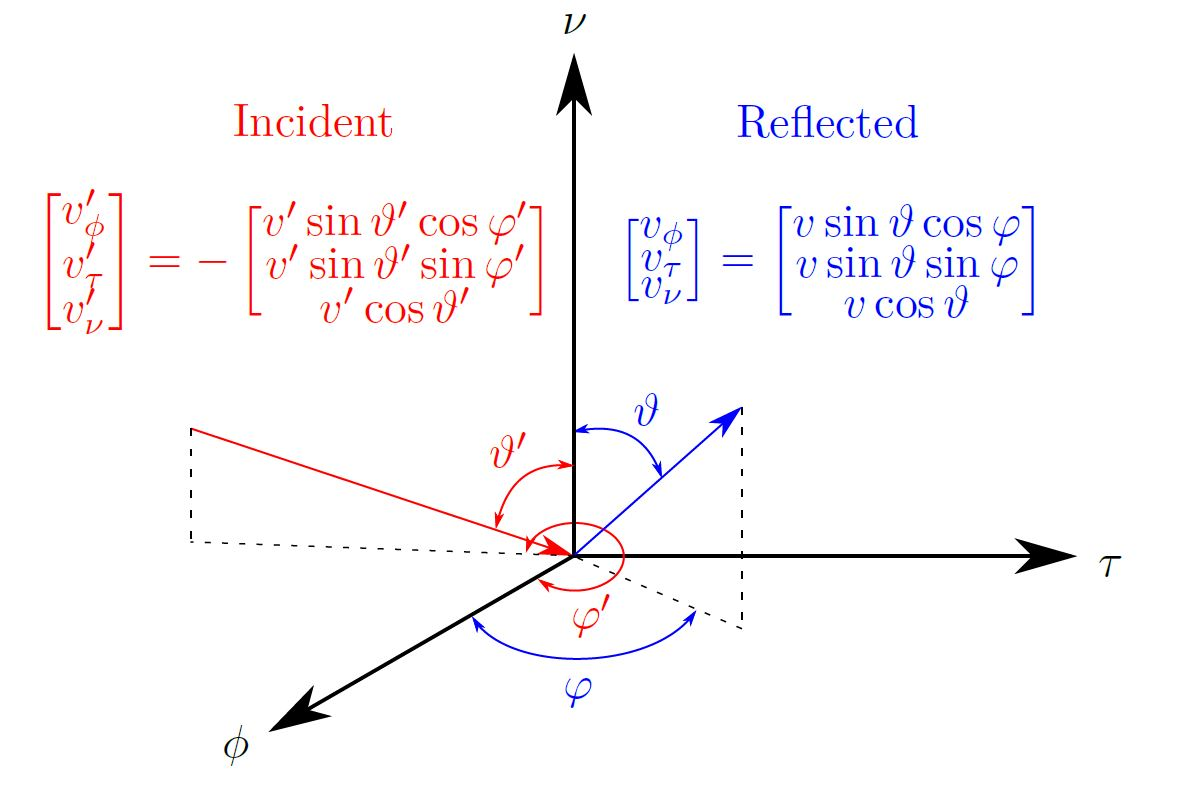
\includegraphics[width = 0.6\textwidth]{Figures/spherical_system.JPG}
	\caption{Transformation from the spherical $(v,\vartheta,\varphi)$ coordinate system to the Cartesian $(\phi,\tau,\nu)$ axis system.}
	\label{fig:spherical}
\end{figure}

We transform the velocity-dependent particle flux densities $\Gamma_{\nu-}^{a}(\xb,\vel')$ and $\Gamma_{\nu+}^{a}(\xb,\vel)$ to their speed- and angle-dependent equivalents $\Gamma_{\nu-}^{a}(\xb,v',\vartheta',\varphi')$ and $\Gamma_{\nu+}^{a}(\xb,v,\vartheta,\varphi)$. $\Gamma_{\nu-}^{a}(\xb,v',\vartheta',\varphi') \dd v' \dd \vartheta' \dd \varphi'$ and $\Gamma_{\nu+}^{a}(\xb,v,\vartheta,\varphi) \dd v \dd \vartheta \dd \varphi$ can be considered as respectively the incident and reflected particle flux densities of species $a$ at position $\xb$ for particles with a speed between $v^{(')}$ and $v^{(')} + \dd v^{(')}$, polar angle between $\vartheta^{(')} $ and $\vartheta^{(')} + \dd \vartheta^{(')}$ and azimuthal angle between $\varphi^{(')}$ and $\varphi^{(')} + \dd \varphi^{(')}$. The parentheses in the superscripts indicate that the prime is optional and only for the incident contribution. The speed- and angle-dependent particle flux density follows from the relation
\begin{align}
\Gamma_{\nu\pm}^{a}\left (\xb,v^{(')},\vartheta^{(')},\varphi^{(')} \right ) \dd v^{(')} \dd \vartheta^{(')} \dd \varphi^{(')} =& \ \Gamma_{\nu\pm}^{a} \left (\xb,\vel^{(')} \right ) \dd \vel^{(')} \nonumber \\
=& \ \Gamma_{\nu\pm}^{a}\left (\xb,\vel^{(')} \right ) \left (v^{(')}\right )^{2} \sin \vartheta^{(')} \dd v^{(')} \dd \vartheta^{(')} \dd \varphi^{(')}. \label{eq:spherical}
\end{align}

Splitting Eq.~\eqref{eq:kineticbc} explicitly into its fast and thermal contributions and using the speed- and angle-dependent distributions, gives

\begin{multline}
\Gammanplus(\xb,v,\vartheta,\varphi) = \int_{v'=0}^{\infty} \int_{\vartheta' = 0}^{\pi/2} \int_{\varphi' = 0}^{2\pi} R_{\mathrm{F}}(\xb;v',\vartheta',\varphi' \rightarrow v,\vartheta,\varphi) \sin \vartheta \ldots \\
\ldots \left( \Ri(\xb) \Gammaimin(\xb,v',\vartheta',\varphi') + \Rnx(\xb) \Gammanmin(\xb,v',\vartheta',\varphi') \right) \dd v' \dd \vartheta' \dd \varphi' \\
+ \frac{1}{\pi} \delta(v-\vT) \cos \vartheta \sin \vartheta \Gammanb{T}(\xb), \quad \text{for} \quad \xb \in \partial D, \label{eq:kineticbc2}
\end{multline}

\noindent with $R_{\mathrm{F}}(\xb;v',\vartheta',\varphi' \rightarrow v, \vartheta, \varphi)$ the fast reflection kernel from the TRIM database, $\delta(v)$ the Dirac delta function, $\vT$ the speed corresponding to the 2-3~eV Franck-Condon energy ($\efc$) and $\Gammanb{T}(\xb)$ the thermal particle flux density, given by
\begin{multline}
\Gammanb{T}(\xb) = \int_{v=0}^{\infty} \int_{\vartheta = 0}^{\pi/2} \int_{\varphi = 0}^{2\pi} \int_{v'=0}^{\infty} \int_{\vartheta' = 0}^{\pi/2} \int_{\varphi' = 0}^{2\pi} (1 - R_{\mathrm{F}}(\xb;v',\vartheta',\varphi' \rightarrow v, \vartheta,\varphi)) \ldots\\
\ldots \sin \vartheta (\Ri(\xb) \Gammaimin(\xb,v',\vartheta',\varphi') + \Rnx(\xb) \Gammanmin(\xb,v',\vartheta',\varphi')) \dd v \dd \theta \dd \phi \dd v' \dd \vartheta' \dd \varphi'. \label{eq:Gammant}
\end{multline}

In Section~\ref{sec:fion}, we determine $\Gammaimin(\xb,v',\vartheta',\varphi')$, which is the distribution of the incident ions. This distribution follows from the plasma solution. Then, we discuss how the fast reflection kernel $R_{\mathrm{F}}(\xb;v',\vartheta',\varphi' \rightarrow v,\vartheta,\varphi)$ is tabulated in the TRIM database in Section~\ref{sec:TRIM}. Finally, we explain in Section~\ref{sec:MCbc} how these boundary conditions are incorporated in the Monte Carlo procedure.

% ----------------------------------------------------------------------
\subsection{Velocity distribution of the incident ions}\label{sec:fion}
% ----------------------------------------------------------------------

Before proceeding to the elaboration of the velocity distribution, we briefly introduce the reader to the sheath boundary physics. At a solid boundary, there is a plasma-wall transition layer. If the magnetic field is oblique to the boundary surface, but with an angle between the magnetic field and surface tangential larger than approximately 5$^{\circ}$, the sheath region can be roughly subdivided in the quasi-neutral magnetic pre-sheath (Chodura sheath), with a width of the order of the ion gyroradius, and the electrostatic sheath (Debye sheath), with a width of the order of the Debye length $\lambda_{\mathrm{D}}$~\cite{chodura1982plasma,stangeby2012chodura}. The Debye length is given by

\begin{equation}
\lambda_{\mathrm{D}} = \left (\frac{\epsilon_{0} \Te}{\nne e^{2}} \right )^{1/2},
\end{equation}

with $\epsilon_{0}$ the permittivity of vacuum and $e$ the elementary charge. At the magnetic pre-sheath entrance, the Chodura condition states that the ion velocity parallel to the magnetic field reaches at least the isothermal speed of sound $\cs = \sqrt{(\Ti + \Te)/m}$. The electric field in the magnetic pre-sheath further accelerates the ions such that also the normal velocity reaches the isothermal speed of sound at the interface between the Chodura and Debye sheath, which is called the Bohm criterion. An extension of the description of the sheath layer for very small angles between the magnetic field and surface tangent (smaller than 5$^{\circ}$) can be found in Refs.~\cite{stangeby2012chodura, tskhakaya2005theory, tskhakaya2014comprehensive}.

The plasma fluid equations are not valid in the sheath region (Chodura and Debye sheaths). Therefore, one typically solves the plasma fluid equations up to the sheath entrance. However, for the neutral simulation, we need an expression for the ion distribution at the boundary surface to evaluate Eqs.~\eqref{eq:kineticbc}, \eqref{eq:kineticbc2}-\eqref{eq:Gammant}. In recent years, there were many efforts in the field of modeling the sheath region~\cite{cohen2004sheath, coulette2016kinetic, tskhakaya2014comprehensive}. However, we use a simplified model that neglects the deflection in the magnetic pre-sheath, similar as in the EIRENE code. It should be noted that the boundary conditions described below can be easily extended to a more elaborated sheath model, once this is implemented and tested in EIRENE.

From now on, we omit the explicit spatial dependence on $\xb$ in the notation. At the sheath entrance, the ion distribution is assumed to be a truncated Maxwellian, leading to

\begin{equation}
\Gamma_{\nu-,\mathrm{se}}^{\mathrm{i}}(\vel_{\mathrm{se}}) = \begin{cases} - C^{\mathrm{i}} \widetilde{M}(\vel_{\mathrm{se}};\Vi,\Ti) (\vel \cdot \Nu) & \text{if} \quad \vel_{\mathrm{se}} \cdot \Nu \leq 0, \\
0 & \text{otherwise}. \end{cases} \label{eq:truncMaxw}
\end{equation}

The constant scaling value $C^{\mathrm{i}}$ follows from the incident ion flux density:
\begin{equation}
\int_{\vel_{\mathrm{se}}} \Gamma_{\nu-,\mathrm{se}}^{\mathrm{i}}(\vel_{\mathrm{se}}) \dd \vel = - \nni (\Vi \cdot \Nu),
\end{equation}
in order to be consistent with the ion continuity equation. In the sheath region, the ions are accelerated perpendicular to the surface by the sheath potential difference $\Delta \phi_{\mathrm{sh}}$. We use the following simplified model for the sheath potential difference~\cite{stangeby1984plasma}:
\begin{equation}\label{eq:shpot}
\Delta \phi_{\mathrm{sh}} = \frac{\dshpot \Te}{e},
\end{equation}
with $\dshpot$ the sheath coefficient. If we express the particle velocity in the $(\phi,\tau,\nu)$ coordinate system of Fig.~\ref{fig:spherical}, then the velocity-dependent particle flux densities at the sheath entrance and boundary are related via
\begin{equation}
\Gamma_{\nu-,\mathrm{se}}^{\mathrm{i}}(v_{\phi,\mathrm{se}},v_{\tau,\mathrm{se}},v_{\nu,\mathrm{se}}) \dd v_{\phi,\mathrm{se}} \dd v_{\tau,\mathrm{se}} \dd v_{\nu,\mathrm{se}} = \Gammaimin(v_{\phi}',v_{\tau}',v_{\nu}') \dd v_{\phi}' \dd v_{\tau}' \dd v_{\nu}'. \label{eq:relationsheath}
\end{equation}
The tangential particle velocity components remain unchanged, i.e., $v_{\phi}' = v_{\phi,\mathrm{se}}$ and $v_{\tau}' = v_{\tau,\mathrm{se}}$, whereas the particle is accelerated by the sheath potential perpendicular to the surface, such that $\frac{m}{2}\left (v_{\nu}'\right )^{2} = \frac{m}{2} v_{\nu,\mathrm{se}}^{2} + \dshpot \Te$. Elaborating Eq.~\eqref{eq:relationsheath}, gives
\begin{equation}
\Gammaimin(v_{\phi}',v_{\tau}',v_{\nu}') = \begin{cases} -C^{\mathrm{i}} \widetilde{M} \Big (v_{\phi}',v_{\tau}',\ldots \\
 \quad \ldots -\sqrt{\left (v_{\nu}'\right )^{2} - \frac{2}{m} \dshpot\Te}; \Vi,\Ti \Big ) v_{\nu}' &  \text{if} \enskip v_{\nu}' \leq -v_{\mathrm{min}}, \\
0 & \text{otherwise}, \end{cases}
\end{equation}
with $v_{\mathrm{min}} = \sqrt{\frac{2}{m}\dshpot \Te}$ the minimum occurring velocity component perpendicular to the boundary after the sheath acceleration, and $\widetilde{M}(v_{\phi},v_{\tau},v_{\nu};{\bf V},T) = \widetilde{M}(\vel;{\bf V},T)$.

This velocity-dependent flux density can be used to evaluate Eq.~\eqref{eq:kineticbc}. However, the TRIM database is given in spherical coordinates (see Section~\ref{sec:TRIM}). Hence, we need an expression of the ion speed- and angle-dependent particle flux density to evaluate Eqs.~\eqref{eq:kineticbc2}-\eqref{eq:Gammant}. Using relation~\eqref{eq:spherical}, gives
\begin{equation}
\Gammaimin(v',\vartheta',\varphi') = \begin{cases} C^{\mathrm{i}} \finorm(v',\vartheta',\varphi';\dshpot) v' \sin \vartheta' \cos \vartheta' & \text{if} \quad v' \geq v_{\mathrm{min}}, \\
& \hspace{0.6cm} \vartheta' \leq \vartheta_{\mathrm{max}}, \\
0 & \text{otherwise}, \end{cases} \label{eq:fib}
\end{equation}
with $\vartheta_{\mathrm{max}} = \arccos (v_{\mathrm{min}}/v')$ and
\begin{multline}
\finorm(v',\vartheta',\varphi';\dshpot) = \left (v' \right )^{2} \widetilde{M} \Bigg (-v' \sin \vartheta' \cos \varphi',-v' \sin \vartheta' \sin \varphi', \ldots \\
\ldots -\sqrt{\left (v'\right )^{2} \cos^{2} \vartheta' -\frac{2}{m} \dshpot \Te};\Vi,\Ti \Bigg ). \label{eq:finormdshpot}
\end{multline}

Now, we have an expression for the speed- and angle-dependent particle flux density for the ions that can be plugged into Eqs.~\eqref{eq:kineticbc2}-\eqref{eq:Gammant}.

% ---------------------------------------------------------------------
\subsection{Reflection kernel from the TRIM database} \label{sec:TRIM}
% ---------------------------------------------------------------------

In this section, we explain how to extract the reflection kernel $R_{\mathrm{F}}(v',\vartheta',\varphi' \rightarrow v,\vartheta,\varphi)$ from the TRIM data tables. We omit the spatial dependence. Moreover, the reflection kernel becomes only spatially dependent if the vessel consists of different materials.

An expression for $R_{\mathrm{F}}(v',\vartheta',\varphi' \rightarrow v,\vartheta,\varphi)$ cannot be directly constructed from the database, because the tables are given as a function of the incident energy and polar angle. Hence, we first find an expression for $R_{\mathrm{F}}(E',\vartheta' \rightarrow E,\cos \vartheta,\cos \delta \varphi)$, with $E' \in [0,\infty]$, $\vartheta' \in [0,\pi/2]$ respectively the kinetic energy and angle with respect to the surface normal of the incident particle, and $E \in [0,E']$, $\vartheta \in [0,\pi/2]$ and $\delta \varphi \in [0, \pi]$ respectively the energy, angle with respect to the surface normal, and azimuthal angle deviation of the reflected/recycled particle. If $\delta \varphi = 0$, the tangential velocity of the recycled/reflected particle is in the same direction as the incident particle, whereas it is in the opposite direction for $\delta \varphi = \pi$.

The TRIM database consists of a total of 84 tables for different combinations of incident energies $E' = 1, 2, 5, 10, 20, 50, 100, 200, 500, 1\,000, 2\,000, \mathrm{and} 5\,000~eV$, and angles $\vartheta' = 0, 30, 45, 60, 70, 80, \mathrm{and} 85$ degrees. Every table contains the value for the particle reflection coefficient $R_{\mathrm{N}}(E',\vartheta')$, defined as
\begin{equation}
R_{\mathrm{N}}(E',\vartheta') = \int_{E = 0}^{E'} \int_{\cos \vartheta = 0}^{1} \int_{\cos \delta \varphi = -1}^{1} R_{\mathrm{F}}(E',\vartheta' \rightarrow E,\cos \vartheta,\cos \delta \varphi) \dd E \dd (\cos \vartheta) \dd (\cos \delta \varphi), \label{eq:RN}
\end{equation}
which is the probability that a particle with energy $E'$ and angle $\vartheta'$ is reflected as a fast atom.

The particle reflection coefficient $R_{\mathrm{N}}(E',\vartheta')$ only gives the probability of fast reflection, but for the distribution regarding the energy and direction of the recycled/reflected particle, we need extra information. For a certain combination of incident particle energy $E'$ and polar angle $\vartheta'$, three conditional distributions are tabulated: i) $R_{\mathrm{F}}(E',\vartheta' \rightarrow E)$ for the reflected energy distribution ($E$); ii) $R_{\mathrm{F}}(E',\vartheta' \rightarrow \cos \vartheta | E)$ for the polar angle distribution ($\cos \vartheta$) knowing that the recycled/reflected particle has energy $E$; and iii) $R_{\mathrm{F}}(E',\vartheta' \rightarrow \cos \delta \varphi | E, \cos \vartheta )$ for the azimuthal angle distribution ($\cos \delta \varphi$) after we know the recycled/reflected energy $E$ and (cosine of) the polar angle $\cos \vartheta$. These conditional distributions follow from
\begin{equation}
R_{\mathrm{F}}(E',\vartheta' \rightarrow E) = \left( \int_{\cos \vartheta = 0}^{1} \int_{\cos \delta \varphi = -1}^{1} R_{\mathrm{F}}(E',\vartheta' \rightarrow E,\cos \vartheta,\cos \delta \varphi) \dd (\cos \vartheta) \dd (\cos \delta \varphi) \right) / R_{\mathrm{N}}(E',\vartheta'),
\end{equation}
% -----------------------------------------------------------------------------------------------
\begin{equation}
R_{\mathrm{F}}(E',\vartheta' \rightarrow \cos \vartheta | E) = \left( \int_{\cos \delta \varphi = -1}^{1} R_{\mathrm{F}}(E',\vartheta' \rightarrow E,\cos \vartheta,\cos \delta \varphi) \dd (\cos \delta \varphi) \right) / \left( R_{\mathrm{N}}(E',\vartheta') R_{\mathrm{F}}(E',\vartheta' \rightarrow E) \right),
\end{equation}
% -------------------------------------------------------------------------------------------------
\begin{align}
R_{\mathrm{F}}(E',\vartheta' \rightarrow \cos \delta \varphi | E, \cos \vartheta ) =& \ R_{\mathrm{F}}(E',\vartheta' \rightarrow E,\cos \vartheta, \cos \delta \varphi)/ \left( R_{\mathrm{N}}(E',\vartheta') \right. \ldots \nonumber \\
\ldots & \left. R_{\mathrm{F}}(E',\vartheta' \rightarrow E) R_{\mathrm{F}}(E',\vartheta' \rightarrow \cos \vartheta | E) \right).
\end{align}
Then, the total reflection kernel can be written as
\begin{align}
R_{\mathrm{F}}(E',\vartheta' \rightarrow E,\cos \vartheta,\cos \delta \varphi) =& R_{\mathrm{N}}(E',\vartheta') R_{\mathrm{F}}(E',\vartheta' \rightarrow E) \ldots \nonumber \\
\ldots & R_{\mathrm{F}}(E',\vartheta' \rightarrow \cos\vartheta | E) R_{\mathrm{F}}(E',\vartheta' \rightarrow \cos \delta \varphi | E, \cos\vartheta).
\end{align}

\noindent These conditional distributions can be considered as three one-dimensional probability density functions. In the TRIM database, these distributions are discretized by means of five quantiles. We generalize the distribution as $R_{\mathrm{F}}(E',\vartheta' \rightarrow x), x \in [x_{\mathrm{min}},x_{\mathrm{max}}]$, with $x = E$ for the conditional energy distribution, $x = \cos \vartheta$ for the polar angle distribution, and $x = \cos \delta \varphi$ for the azimuthal angle distribution. Then, the cumulative distribution $F_{\mathrm{F}}(E',\vartheta' \rightarrow x)$ is defined as
\begin{equation}
F_{\mathrm{F}}(E',\vartheta' \rightarrow x) = \int_{x_{\mathrm{min}}}^{x} R_{\mathrm{F}}(E',\vartheta' \rightarrow y) \dd y.
\end{equation}
This distribution is discretized with five quantiles:
\begin{equation}
F_{\mathrm{F}}(E',\vartheta' \rightarrow x_{i}) = q_{i}, \quad \text{for} \quad i = 1, \ldots 5,
\end{equation}
with $q_{i} = 0.1 + 0.2(i-1)$. This is illustrated in Fig.~\ref{fig:reflection} (a), where the blue line represents the real cumulative distribution. The linear interpolation between these quantiles leads to a piecewise constant approximation for the probability density functions, as can be seen in Fig.~\ref{fig:reflection} (b).
\begin{figure}[ht]
	\centering
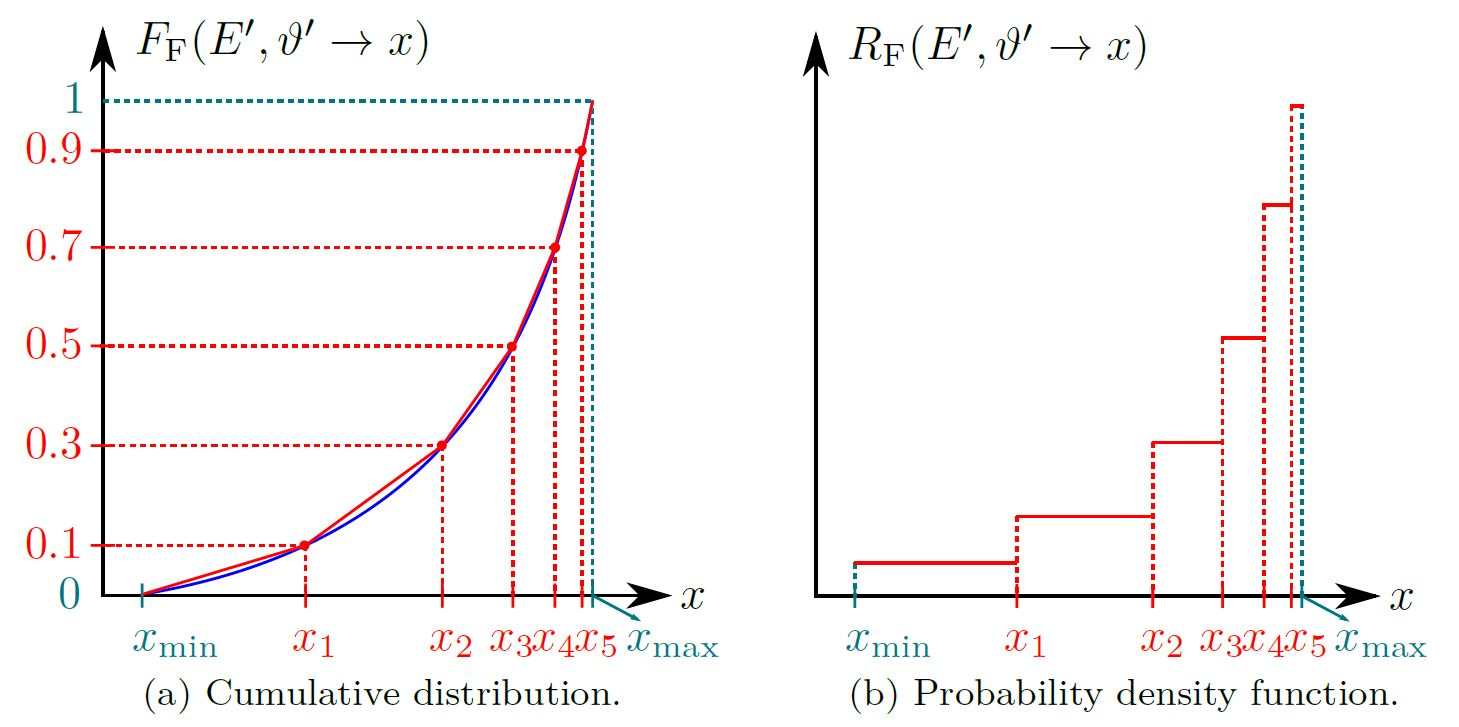
\includegraphics[width = 1.0\textwidth]{Figures/quantiles.JPG}
	\caption{Conditional cumulative distribution and probability density function from the TRIM database.}
 \label{fig:reflection}
\end{figure}

\noindent The cumulative distribution $F_{\mathrm{F}}(E',\vartheta' \rightarrow E)$ is discretized with five quantiles $E_{i}$ for every value of $E'$ and $\vartheta'$. Then for every quantile $E_{i}$, the function $F_{\mathrm{F}}(E',\vartheta' \rightarrow \cos \vartheta | E_{i})$ is discretized with five quantiles $\cos \vartheta_{j}$, thus, 25 additional numbers. Finally, the same is done for $F_{\mathrm{F}}(E',\vartheta' \rightarrow \cos \delta \varphi |E_{i}, \cos \vartheta_{j}$ (125 additional numbers). Hence, for every combination of $E'$ and $\vartheta'$ the TRIM database contains 155 numbers + 1 additional number for the reflection coefficient. Fig.~\ref{fig:trim} shows an example of a table from the TRIM database for a given incident energy-angle combination. The last number of the first line is the reflection coefficient $R_{\mathrm{N}}(E',\vartheta')$. The second line contains the quantiles for the reflected energy, the next five lines the quantiles for $\cos \vartheta$ for every value of $E$, and the next 25 lines contain the quantiles for $\cos \delta \varphi$ for every combination of $E$ and $\cos \vartheta$.

\begin{figure}[H]
	\centering
%	\def\svgwidth{160pt}
	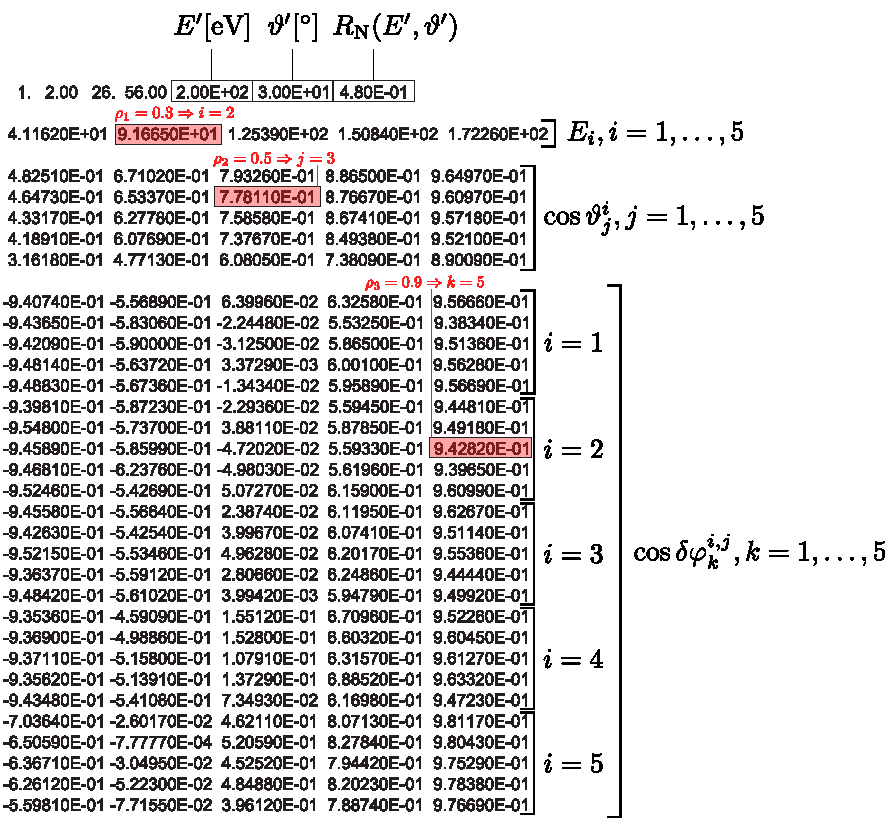
\includegraphics[width = 1.0\textwidth ]{Figures/trim.pdf}
	\caption[Data block from the TRIM database for $E' = 200$~eV and $\vartheta' = 30^{\circ}$.]{Data block from the TRIM database for $E' = 200$~eV and $\vartheta' = 30^{\circ}$~\cite{reiter2009eirene}.}
	\label{fig:trim}
\end{figure}

From the expression for $R_{\mathrm{F}}(E',\vartheta' \rightarrow E,\cos \vartheta, \cos \delta \varphi)$ we can derive the reflection kernel $R_{\mathrm{F}}(v',\vartheta',\varphi' \rightarrow v,\vartheta, \varphi)$ in Eq.~\eqref{eq:kineticbc2}, via the relation

\begin{equation}
R_{\mathrm{F}}(v',\vartheta',\varphi' \rightarrow v, \vartheta, \varphi) \sin \vartheta \dd v \dd \vartheta \dd \varphi = \frac{1}{2}R_{\mathrm{F}}(E',\vartheta' \rightarrow E, \cos \vartheta, \cos \delta \varphi) \dd E \left| \dd (\cos \vartheta) \dd (\cos \delta \varphi) \right| .
\end{equation}

In the right hand side, there appears a factor $1/2$, because of the equal probability that the particle is azimuthally deviating in the clockwise or counterclockwise directions compared to its original trajectory. With
\begin{equation}
E' = \frac{m}{2} (v')^{2}, \quad E = \frac{m}{2} v^{2}, \quad \varphi = \varphi' + \pi \pm \delta \varphi,
\end{equation}
this becomes
\begin{equation}
R_{\mathrm{F}}(v',\vartheta',\varphi' \rightarrow v, \vartheta, \varphi) = \frac{m}{2} v \left| \sin (\varphi - \varphi') \right| R_{\mathrm{F}} \left( \frac{m}{2} (v')^{2},\vartheta' \rightarrow \frac{m}{2} v^{2},\cos \vartheta, \cos (\varphi - \varphi') \right).
\end{equation}

% ---------------------------------------------------------------------
\subsection{Treatment of boundary conditions in Monte Carlo simulation} \label{sec:MCbc}
% ---------------------------------------------------------------------

\subsubsection{Application of the TRIM database}

The specific format for the TRIM tables facilitates the Monte Carlo simulation for the reflection of particles at a boundary. If a particle hits a boundary, its energy and incident polar angle are calculated. Then, the reflection coefficient $R_{\mathrm{N}}$ is determined by means of linear interpolation or extrapolation of the TRIM data. A random number $\rho$ from a uniform distribution between 0 and 1 is generated. If $\rho \leq R_{\mathrm{N}}$ the particle is reflected as a fast atom and the TRIM database is applied (option~1 below), otherwise the particle is thermally released (option~2 below).

\begin{itemize}
	\item \emph{Option~1: fast reflection.} Three uniformly distributed random numbers $\rho_{1}$, $\rho_{2}$ and $\rho_{3}$ (between 0 and 1) are generated. They determine respectively the reflected energy, polar angle and azimuthal angle. The reflected energy follows from
	\begin{equation}
	F_{\mathrm{F}}(E',\vartheta' \rightarrow E ) = \rho_{1},
	\end{equation}
	with the piecewise linear approximation of the cumulative distribution (Fig.~\ref{fig:reflection}(a)). Then, the polar angle is determined by
	\begin{equation}
	F_{\mathrm{F}}(E',\vartheta' \rightarrow \cos \vartheta | E) = \rho_{2},
	\end{equation}
	and finally, the relation for the azimuthal angle is
	\begin{equation}
	F_{\mathrm{F}}(E',\vartheta' \rightarrow \cos \delta \varphi | E,\cos \vartheta ) = \rho_{3}.
	\end{equation}
	
	For the three random numbers $\rho_{1} = 0.3$, $\rho_{2} = 0.5$ and $\rho_{3} = 0.9$ and an incident energy of 200~eV and polar angle of $30^{\circ}$ for the target-projectile combination of Fig.~\ref{fig:trim}, the resulting reflected energy and angles are indicated in the figure. For intermediate values of $E'$ and $\vartheta'$ and random numbers that do not exactly correspond with a tabulated quantile, linear interpolation/extrapolation of the tables is used.
	
	\item \emph{Option~2: thermal release.} In case of thermal release, the particle gets an energy of 2-3~eV. In order to have an isotropically distributed surface source (Lambert's cosine law), the polar angle has to be sampled from the probability density function $f(\vartheta)$, given by
	\begin{equation}
	f(\vartheta) = 2 \cos \vartheta \sin \vartheta, \quad \text{for} \quad \vartheta \in [0,\pi/2],
	\end{equation}
	as can be seen in Eq.~\eqref{eq:kineticbc2}~\cite{greenwood2002correct}. The corresponding cumulative distribution is
	\begin{eqnarray}
	F(\vartheta) &=& \int_{0}^{\vartheta} f(\vartheta') \dd \vartheta' \nonumber \\
	&=& \sin^{2} \vartheta.
	\end{eqnarray}
\noindent	Then, the polar angle follows from the relation
	\begin{equation}
	F(\vartheta) = \rho,
	\end{equation}
\noindent	with $\rho$ a random number uniformly distributed between 0 and 1. This leads to
	\begin{equation}
	\vartheta = \arcsin(\sqrt{\rho}).
	\end{equation}
\noindent	The azimuthal reflected angle is uniformly sampled between 0 and $2\pi$.
\end{itemize}

% ------------------------------------------------------
\section{Fluid boundary conditions} \label{sec:fluidbc}
% ------------------------------------------------------

In this section, we derive the boundary conditions for the fluid neutral models. The fluid models as described in literature use simple boundary conditions. E.g., a typical boundary condition for the parallel momentum equation is the momentum recycling boundary condition where the neutral parallel velocity at the target plate is assumed to be a constant fraction of the ion parallel velocity~\cite{rensink1998comparison,riemann2004navier}. However, this fraction is user-defined and not based on the underlying physics.

Here, we carefully derive the boundary conditions from the underlying kinetic physics. This is done by taking the particular moments of the neutral velocity distribution at the boundary. The total distribution consists of three parts: the incident neutrals, the reflected neutrals (an incident atom that is reflected as a fast or thermal atom) and the recycled neutrals (the incident ions that pick up an electron and are emitted as fast or thermal atoms). The distribution of the recycled neutrals can be calculated by taking the ion distribution at the boundary that entirely follows from the plasma macroscopic properties (Eq.~\eqref{eq:fib}), and multiplying it by the reflection kernel and integrating this product over the incident velocity space (Eqs.~\eqref{eq:kineticbc2}-\eqref{eq:Gammant}). The story is different for the reflected neutrals, because we need an expression for the distribution of the incident neutrals, but this can only be known by solving the kinetic equation. For the fluid models, we make an estimate for the distribution of these incident atoms.

The estimate is based on the diffusion approximation, as explained in Section~\ref{sec:diff}, or the drifting Maxwellian approximation, as explained in Section~\ref{sec:maxwellian}. Again, applying the reflection kernel leads to an estimate for the distribution of the reflected particles. In Section~\ref{sec:boundaryfluxes}, we take moments from the total distribution to obtain macroscopic fluxes. Finally, Section~\ref{sec:bcimplementation} deals with the practical implementation of these boundary conditions with imposed fluxes. It should be noted that the error introduced by the boundary conditions is fully due to the approximation for the incident neutrals. The TRIM reflection model is used for both the fluid and kinetic models and consequently, it does not introduce additional errors.


% ------------------------------------------------------
\subsection{Diffusion approximation for the distribution of the incident neutrals} \label{sec:diff}
% ------------------------------------------------------

Diffusion theory is frequently used in nuclear (fission) reactor physics~\cite{espinosa2011fractional, lamarsh1966introduction, park2012generation, piovezan2013heavy}. In our case, we will exclusively use it to estimate the distribution of the incident neutrals. We consider a control volume $\dd \mathcal{V}$ in which charge-exchange collisions scatter the neutrals in different directions, as indicated in Fig.~\ref{fig:diffusion}. We are interested in the number of neutrals that reach the area $\dd \mathcal{A}$ spanned by the solid angle $\dd \Omega$. $\dd \mathcal{A}$ is a surface element of the boundary (e.g., the target plate).
\begin{figure}[H]
	\centering
	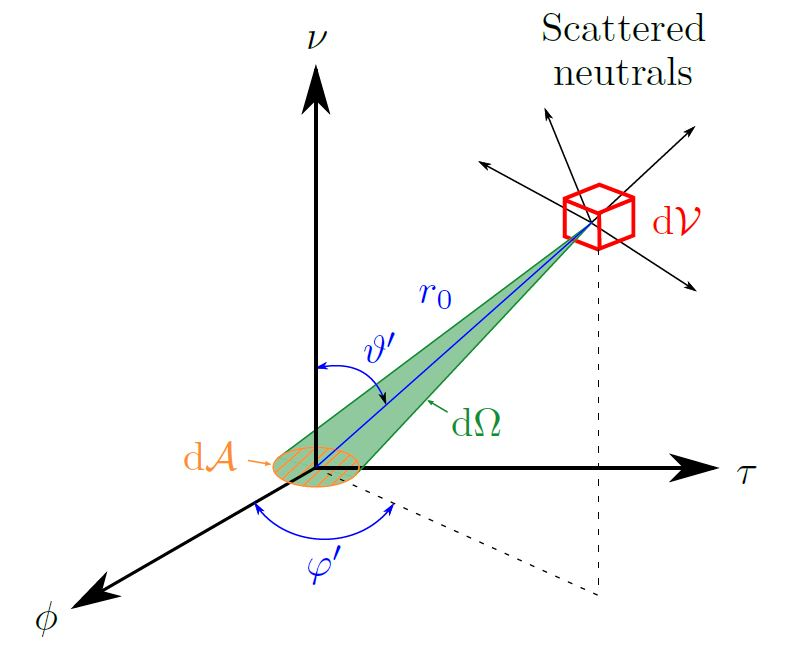
\includegraphics[width=0.5\textwidth]{Figures/scattering.JPG}
	\caption[Scattering of neutrals in control volume $\dd \mathcal{V}$.]{Scattering of neutrals in control volume $\dd \mathcal{V}$~\cite{nf_niels}.}
	\label{fig:diffusion}
\end{figure}

We calculate the speed- and angle-dependent particle flux density $\Gammanmin(v',\vartheta',\varphi')$ of neutrals scattered by the ions and reaching the plane $\dd \mathcal{A}$. We interpret $\Gammanmin(v',\vartheta',\varphi') \dd v' \dd \vartheta' \dd \varphi'$ as the number of neutrals per unit area per second reaching the surface element $\dd \mathcal{A}$ with a polar angle between $\vartheta'$ and $\vartheta' + \dd \vartheta'$, an azimuthal angle between $\varphi'$ and $\varphi' + \dd \varphi'$, and a speed between $v'$ and $v' + \dd v'$.

To calculate $\Gammanmin(v',\vartheta',\varphi')$, we need the source $S(v',\vartheta',\varphi')$ of neutrals created in the volume element $\dd \mathcal{V}$ with a speed between $v'$ and $v' + \dd v'$ scattered in the solid angle $\dd \Omega$. Charge-exchange collisions are assumed to be the main origin for neutral particles at a certain distance $r_{0}$. Thus, the source can be written as
\begin{equation}
S(v',\vartheta',\varphi') = \nn \nni \rcxm \finorm(v',\vartheta',\varphi'), \label{eq:S}
\end{equation}
which is the number of charge-exchange collisions per unit volume per second, multiplied with the normalized ion distribution $\finorm(v',\vartheta',\varphi')$. Here, $\nn$ is the neutral particle density, $\nni$ is the ion particle density, and $\rcxm$ is the momentum-linearized charge-exchange rate, as defined in Ref. \cite{nf_niels}.

The ion distribution in the domain is assumed to be a drifting Maxwellian $\left( \finorm(\vel') = \widetilde{M}(\vel';\Vi,\Ti) \right)$. This ion distribution is expressed as a function of the three velocity components and has to be transformed to the speed- and angle-dependent distribution as a function of $v'$, $\vartheta'$ and $\varphi'$. This is done with the transformation from Cartesian to spherical coordinates:
\begin{equation}
\finorm(\vel') \dd \vel' = \finorm(\vel') \left (v' \right )^{2} \dd v' \dd \Omega = \finorm(v',\vartheta',\varphi') \dd v' \dd \Omega.
\end{equation}
In this way, $\finorm(v',\vartheta',\varphi')$ becomes
\begin{align}
\finorm(v',\vartheta',\varphi') =& \left (v'\right )^{2} \widetilde{M}(\vel';\Vi,\Ti) \nonumber \\
=& \left (v'\right )^{2} \left( \frac{m}{2\pi\Ti} \right)^{3/2} \exp \left( -\frac{m}{2\Ti} \left( \left( v_{\phi}' - \ww \right)^{2} + \left(v_{\tau}' - u_{\tau} \right)^{2} + \left( v_{\nu}' - u_{\nu} \right)^{2} \right) \right).
\end{align}
Also transforming the Cartesian particle velocities to spherical coordinates, gives
\begin{multline}
\finorm(v',\vartheta',\varphi') = \left (v' \right)^{2} \left( \frac{m}{2\pi\Ti}\right)^{3/2} \times \\
\times \exp \left( -\frac{m}{2\Ti} \left( \left( v' \right)^{2} + 2 v' \sin \vartheta' \sin \varphi' u_{\tau} + 2 v' \sin \vartheta' \cos \varphi' u_{\phi} + 2 v' \cos \vartheta' u_{\nu} + u_{\phi}^{2} + u_{\tau}^{2} + u_{\nu}^{2} \right) \right). \label{eq:finorm}
\end{multline}

\noindent This source has to be multiplied with the probability that the neutral reaches the boundary plane without any extra collision (probability of non-absorption $P_{\mathrm{NA}}(v')$). This probability is given by
\begin{equation}
P_{\mathrm{NA}}(v') = \exp \left( -\St(v') r_{0} \right), \label{eq:PNA}
\end{equation}
with $\St(v') = (\nni\rcxm + \nne\rion)/v'$ the total macroscopic cross-section (including charge-exchange and ionization events).

Then, the speed- and angle-dependent particle flux density becomes
\begin{equation}
\Gammanmin(v',\vartheta',\varphi') \dd v' \dd \vartheta' \dd \varphi' \dd \mathcal{A} = \int_{\mathcal{V}} S(v',\vartheta',\varphi') P_{\mathrm{NA}}(v') \dd \mathcal{V} \dd v' \dd \Omega. \label{eq:Gammanmin1}
\end{equation}
To obtain the total particle flux density, the integral over the whole domain volume has to be taken. If the total macroscopic cross-section is large, the exponential term $e^{-\St(v') r_{0}}$ in $P_{\mathrm{NA}}(v')$ (Eq.~\eqref{eq:PNA}) decays rapidly. Therefore, only the first few mean free paths starting from the boundary contribute to the integral of Eq.~\eqref{eq:Gammanmin1}, and we can replace the integral over the edge plasma domain by a semi-infinite integral with $r_{0} \in [0,\infty )$. The solid angle spanned by $\dd \mathcal{A}$ is $\dd \mathcal{A} \frac{\cos\vartheta'}{r_{0}^{2}}$ and the volume $\dd \mathcal{V}$ is $r_{0}^{2}\sin \vartheta' \dd r_{0} \dd \vartheta' \dd \varphi'$. Inserting all expressions in Eq.~\eqref{eq:Gammanmin1}, gives
\begin{equation}
\Gammanmin(v',\vartheta',\varphi') = \int_{r_{0}=0}^{\infty} e^{-\St(v') r_{0}} \nn \nni \rcxm \finorm(v',\vartheta',\varphi') \sin \vartheta' \cos \vartheta' \dd r_{0}. \label{eq:Gammanmin2}
\end{equation}
We use a Taylor series expansion for the neutral density:
\begin{eqnarray}
\nn &\approx& n_{\mathrm{n}_{0}} + \phi \left (\ddx{\nn}{\phi}\right )_{0} + \tau \left (\ddx{\nn}{\tau}\right )_{0} + \nu \left (\ddx{\nn}{\nu} \right )_{0} \nonumber \\
&=& n_{\mathrm{n}_{0}} + r_{0} \sin \vartheta' \sin \varphi' \left (\ddx{\nn}{\tau}\right )_{0}  + r_{0} \cos \vartheta' \left (\ddx{\nn}{\nu} \right )_{0},
\end{eqnarray}
assuming toroidal symmetry such that $(\partial \nn/\partial \phi)_{0} = 0$. The subscript 0 indicates that the neutral density and gradients are evaluated in the origin, where the particle flux density is calculated. Inserting this expression for the neutral density in Eq.~\eqref{eq:Gammanmin2}, gives
\begin{align}
\Gammanmin(v',\vartheta',\varphi') = \int_{r_{0}=0}^{\infty} & e^{-\St(v') r_{0}} \left( \nn + r_{0} \sin \vartheta' \sin \varphi' \left( \ddx{\nn}{\tau} \right) + r_{0} \cos \vartheta' \left( \ddx{\nn}{\nu}\right) \right) \times \nonumber \\
\times & \nni \rcxm \finorm(v',\vartheta',\varphi') \sin \vartheta' \cos \vartheta' \dd r_{0}, \label{eq:Gammanmin3}
\end{align}
where the subscript $0$ is omitted for simplicity of notation. Finally, evaluating the integral neglecting the spatial dependence of $\St$, $\nni \rcxm$, and $\finorm$, gives
\begin{align}
\Gammanmin(v',\vartheta',\varphi') =& \frac{\nni \rcxm}{\nni \rcxm + \nne \rion} \finorm(v',\vartheta',\varphi') v' \sin \vartheta' \cos \vartheta' \times \nonumber \\
\times & \left( \nn + \frac{v'}{\nni\rcxm + \nne \rion} \left( \sin \vartheta' \sin \varphi' \ddx{\nn}{\tau} + \cos \vartheta' \ddx{\nn}{\nu} \right) \right) \label{eq:Gammanmin}
\end{align}

Due to the exponential decay term in Eq.~\eqref{eq:Gammanmin3}, only the first mean free paths away from the boundary contribute to the integral and the spatial variations of $\St$, $\nni\rcxm$, and $\finorm$ can be assumed to be small in this region. Basically, this means that the Knudsen number has to be sufficiently small, which is also a necessary condition for the use of a fluid model in the bulk of the domain. Indeed, a small Knudsen number means that the macroscopic length scales of the parameters in the integrand of Eq.~\eqref{eq:Gammanmin3} are large compared to the neutral mean free path length ($1/\St$). These large macroscopic length scales compared to the mean free path length lead to relatively small variations of the macroscopic properties in the exponentially decaying region that contributes to the integral.

% ------------------------------------------------------
\subsection{Truncated drifting Maxwellian approximation for the distribution of the incident neutrals} \label{sec:maxwellian}
% ------------------------------------------------------

The diffusion approximation for the incident neutrals was shown to be accurate for the target boundary conditions in \cite{nf_niels} and \cite{pet_maarten}. However, this boundary condition requires a short mean free path to be valid, and it was found that unphysical behavior can arise when the mean free path is too long. Therefore, an alternative model was developed, assuming a truncated drifting Maxwellian distribution for the incident neutrals, based on the macroscopic neutral density, velocity, and temperature at the target:

\begin{align}
\Gammanmin(v',\vartheta',\varphi') =&  \fnnorm(v',\vartheta',\varphi') v' \sin \vartheta' \cos \vartheta'. \label{eq:Gammanmin_maxw}
\end{align}

Here, the normalized neutral distribution is
\begin{align}
\fnnorm(v',\vartheta',\varphi') =& \left( v' \right)^{2} \widetilde{M} (\vel';\Vn,\Tn) \nonumber \\
=& \left( v' \right)^{2} \left( \frac{m}{2\pi\Tn} \right)^{3/2} \exp \left( -\frac{m}{2\Tn} \left( \left( v_{\phi}' - \wwn \right)^{2} + \left( v_{\tau}' - u_{\mathrm{n}\tau} \right)^{2} + \left( v_{\nu}' - u_{\mathrm{n}\nu} \right)^{2} \right) \right).
\end{align}

Again transforming the Cartesian particle velocities to spherical coordinates, gives
\begin{multline}
\fnnorm(v',\vartheta',\varphi') = \left (v'\right )^{2} \left (\frac{m}{2\pi\Tn}\right )^{3/2} \exp \bigg (-\frac{m}{2\Tn} \Big (\left (v'\right )^{2} + 2 v' \sin \vartheta' \sin \varphi' u_{\mathrm{n}\tau} + \\
+ 2 v' \sin \vartheta' \cos \varphi' u_{\mathrm{n}\phi}
+ 2 v' \cos \vartheta' u_{\mathrm{n}\nu} + u_{\mathrm{n}\phi}^{2} + u_{\mathrm{n}\tau}^{2} + u_{\mathrm{n}\nu}^{2} \Big ) \bigg ). \label{eq:fnnorm}
\end{multline}

This option was found to be slightly less accurate than the diffusion approximation for high collisional cases \cite{nf_wim}, but still far more accurate than previous {\it ad hoc} fluid neutral boundary conditions, while being more robust in the regions with larger neutral mean free paths.
From now on, we use the superscripts `diff' and `Maxw' to differentiate between the diffusion and Maxwellian options, when the distinction needs to be made explicit.

% ------------------------------------------------------
\subsection{Resulting macroscopic boundary fluxes} \label{sec:boundaryfluxes}
% ------------------------------------------------------

From the distributions of the incident neutrals and ions, the net fluxes at the boundaries can be calculated. In our case, the speed and angular distributions of the fast recycled and reflected neutrals are determined by the TRIM code database, whereas the thermally released neutrals are emitted diffusely with an energy of 2-3~eV. Below, we elaborate the particle, parallel momentum, and energy flux density.

% ------------------------------------------------------
\subsubsection{Neutral particle flux density}

\noindent The net neutral particle flux density $\Gamma^{\mathrm{n}} = \nn \Vn \cdot \Nu$ constitutes of four contributions:
\begin{equation}
\Gamma^{\mathrm{n}} =  \Gamma_{\mathrm{refl},\mathrm{f}}^{\mathrm{n}} + \Gamma_{\mathrm{rec},\mathrm{f}}^{\mathrm{n}} + \Gammanb{T} - \Gamma_{\nu-}^{\mathrm{n}},
\end{equation}
with $\Gamma_{\mathrm{refl},\mathrm{f}}^{\mathrm{n}}$ and $\Gamma_{\mathrm{rec},\mathrm{f}}^{\mathrm{n}}$ respectively the fast reflected and recycled particle flux density (as described by the TRIM database) and $\Gammanb{T}$ the thermally released fraction, decreased with the incident particle flux density $\Gamma_{\nu-}^{\mathrm{n}}$. These contributions are elaborated with the help of the particle reflection coefficient (Eq.~\eqref{eq:RN}):
\begin{align}
\Gamma_{\nu-}^{\mathrm{n}} =& \int_{v'=0}^{\infty} \int_{\vartheta'=0}^{\pi/2} \int_{\varphi'=0}^{2\pi} \Gamma_{\nu-}^{\mathrm{n}}(v',\vartheta',\varphi') \dd v' \dd \vartheta' \dd \varphi', \label{eq:Gammanin} \\
\Gamma_{\mathrm{refl},\mathrm{F}}^{\mathrm{n}} =& \ \Rnx \int_{v'=0}^{\infty} \int_{\vartheta'=0}^{\pi/2} \int_{\varphi'=0}^{2\pi} R_{\mathrm{N}}(v',\vartheta') \Gamma_{\nu-}^{\mathrm{n}}(v',\vartheta',\varphi') \dd v' \dd \vartheta' \dd \varphi', \label{eq:Gammarefl} \\
\Gamma_{\mathrm{rec},\mathrm{F}}^{\mathrm{n}} =& \ \Ri \int_{v'=0}^{\infty} \int_{\vartheta'=0}^{\pi/2} \int_{\varphi'=0}^{2\pi} R_{\mathrm{N}}(v',\vartheta') \Gamma_{\nu-}^{\mathrm{i}}(v',\vartheta',\varphi') \dd v' \dd \vartheta' \dd \varphi', \label{eq:Gammarec}
\end{align}
\begin{align}
\Gammanb{T} = \int_{v'=0}^{\infty} \int_{\vartheta'=0}^{\pi/2} \int_{\varphi'=0}^{2\pi} \left( 1 - R_{\mathrm{N}}(v',\vartheta') \right) \left( \Rnx \Gammanmin(v',\vartheta',\varphi') + \Ri \Gammaimin(v',\vartheta',\varphi') \right) \dd v' \dd \vartheta' \dd \varphi'. \label{eq:GammanT}
\end{align}

It should be noted that the particle reflection coefficient is written as a function of the incident speed $v'$ and not as function of the incident energy $E' = \frac{m}{2}(v')^{2}$ in Eq.~\eqref{eq:RN}.

% -------------------------------------------------------
\subsubsection{Neutral parallel momentum flux density}


Similar to the net neutral particle flux density, the neutral parallel momentum flux density $\Gamma_{\mathrm{m},||}^{\mathrm{n}}$ becomes

\begin{align}
\Gamma_{\mathrm{m},||}^{\mathrm{n}} =& \left[ \left( m\nn\Vn\Vn + \viscn + \pn \mathds{I} \right) \cdot \Nu \right]_{||} \label{eq:momfluxp} \\
=& \ m \int_{v'=0}^{\infty} \int_{\vartheta'=0}^{\pi/2} \int_{\varphi'=0}^{2\pi} \Bigg [ \underbrace{-v'_{||} \Gamma_{\nu-}^{\mathrm{n}}(v',\vartheta',\varphi')}_{\text{incident}} \nonumber \\
& + \underbrace{\int_{v=0}^{v'} \int_{\vartheta=0}^{\pi/2} \int_{\varphi=0}^{2\pi} v_{||}  R_{\mathrm{F}}(v',\vartheta',\varphi' \rightarrow v, \vartheta,\varphi)\sin \vartheta \dd v \dd \vartheta \dd \varphi\ldots}_{\text{fast}} \nonumber \\
&\qquad \underbrace{\ldots \left (\Rnx \Gamma_{\nu-}^{\mathrm{n}}(v',\vartheta',\varphi') + \Ri \Gamma_{\nu-}^{\mathrm{i}}(v',\vartheta',\varphi')\right )}_{\text{fast}} \Bigg ] \dd v' \dd \vartheta' \dd \varphi' + \underbrace{\Gamma_{\mathrm{m},||,\mathrm{T}}^{\mathrm{n}}}_{\text{thermal}}, \label{eq:Gammamp}
\end{align}

\noindent with $v_{||} = \pit (\sin \alpha_{\nu} v_{\tau} + \cos \alpha_{\nu} v_{\nu}) + \pitt v_{\phi}$ the neutral particle velocity parallel to the magnetic field, and $\alpha_{\nu}$ the angle between the surface normal and the poloidal direction. The different contributions are indicated with sub braces. To write Eq.~\eqref{eq:Gammamp} more compactly, we make use of the parallel and perpendicular momentum reflection coefficients, respectively $R_{\mathrm{m},||}(v',\vartheta')$ and $R_{\mathrm{m},\perp}(v',\vartheta')$. Then, Eq.~\eqref{eq:Gammamp} becomes
\begin{align}
\Gamma_{\mathrm{m},||}^{\mathrm{n}} =& \ m \int_{v'=0}^{\infty} \int_{\vartheta'=0}^{\pi/2} \int_{\varphi'=0}^{2\pi} \Bigg[ \underbrace{- v'_{||} \Gamma_{\nu-}^{\mathrm{n}}(v',\vartheta',\varphi')}_{\text{incident}} +  \underbrace{\bigg (- \pitt R_{\mathrm{m},||}(v',\vartheta') \ldots}_{\text{fast}}  \nonumber \\
& \underbrace{\ldots  \sin \vartheta' \cos \varphi' - \pit \sin \alpha_{\nu} R_{\mathrm{m},||}(v',\vartheta') \sin \vartheta' \sin \varphi' + \pit \cos \alpha_{\nu}  \ldots}_{\text{fast}} \nonumber \\
&\underbrace{\ldots R_{\mathrm{m},\perp}(v',\vartheta') \cos \vartheta' \bigg ) v' \left( \Rnx \Gamma_{\nu-}^{\mathrm{n}}(v',\vartheta',\varphi') + \Ri \Gamma_{\nu-}^{\mathrm{i}}(v',\vartheta',\varphi') \right)}_{\text{fast}} \Bigg] \dd v' \dd \vartheta' \dd \varphi' + \ldots \nonumber \\
&\ldots + \underbrace{\Gamma_{\mathrm{m},||,\mathrm{T}}^{\mathrm{n}}}_{\text{thermal}}, \label{eq:Gammanmomp}
\end{align}
with
\begin{align}
R_{\mathrm{m},||}(v',\vartheta') = \frac{1}{mv'\sin\vartheta'} \int_{v=0}^{v'} \int_{\vartheta=0}^{\pi/2}\int_{\varphi=0}^{2\pi} m v \sin\vartheta \cos \varphi R_{\mathrm{F}}(v',\vartheta',0 \rightarrow v,\vartheta,\varphi) \sin \vartheta \dd v \dd \vartheta \dd \varphi, \label{eq:Rmpar}
\end{align}
\begin{align}
R_{\mathrm{m},\perp}(v',\vartheta') = \frac{1}{mv'\cos \vartheta'} \int_{v=0}^{v'} \int_{\vartheta=0}^{\pi/2} \int_{\varphi=0}^{2\pi} m v \cos \vartheta R_{\mathrm{F}}(v',\vartheta',0 \rightarrow v,\vartheta,\varphi) \sin \vartheta \dd v \dd \vartheta \dd \varphi. \label{eq:Rmperp}
\end{align}

The parallel momentum reflection coefficient represents the mean fraction of momentum that is conserved in the direction of motion of the incident particle projected on the boundary plane multiplied by the probability of fast reflection $R_{\mathrm{N}}(v',\vartheta')$. The perpendicular momentum reflection coefficient represents the ratio of the momentum perpendicular to the plane of the reflected and incident particle again multiplied by $R_{\mathrm{N}}(v',\vartheta')$. The calculation of these reflection coefficients is treated in Section~\ref{sec:bcimplementation}.

The thermally released neutrals are emitted isotropically (Lambert's cosine law), leading to the following parallel momentum flux density:
\begin{align}\label{eq:par_momentum_T}
\Gamma_{\mathrm{m},||,\mathrm{T}}^{\mathrm{n}} =& \ m \int_{v=0}^{\infty} \int_{\vartheta = 0}^{\pi/2} \int_{\varphi = 0}^{2\pi} v_{||} \frac{1}{\pi} \delta(v - \vT) \cos \vartheta \sin \vartheta \Gammanb{T} \nonumber \\
=& \ \pit \cos \alpha_{\nu} \frac{2}{3} m \vT \Gammanb{T}.
\end{align}

As can be seen in Eq.~\eqref{eq:momfluxp}, this parallel momentum flux density includes the pressure. However, for fluid models, it is typical to consider the pressure gradient as a driving force rather than a flux contribution. The parallel momentum flux density from the fluid point of view (subscript $\mathrm{f}$) becomes
\begin{equation}
\Gamma_{\mathrm{m},\mathrm{f},||}^{\mathrm{n}} = \left [\Gamma_{\mathrm{m,f}}^{\mathrm{n}} \cdot \Nu\right ]_{||} = \Gamma_{\mathrm{m},||}^{\mathrm{n}} - \pit \cos \alpha_{\nu} \pn, \label{eq:Gammamompf}
\end{equation}
i.e., excluding the pressure contribution.

There are two possible choices for the pressure at a certain position at a boundary. One can take the pressure that follows from the fluid solution. However, at the boundaries, the underlying velocity distribution deviates a lot from the Maxwellian equilibrium distribution. Therefore, it is recommended to recalculate the pressure from the estimated distribution that consists of the incident, recycled, and reflected neutrals. If the total velocity-dependent particle flux density at a boundary is $\Gamma^{\mathrm{n}}(\vel)$, the pressure is defined as
\begin{equation}
\pn' = \frac{m}{3} \int ||\vel -\Vn'||^{2} \frac{\Gamma^{\mathrm{n}}(\vel)}{|v_{\nu}|} \dd \vel, \label{eq:pnboundary}
\end{equation}
where the prime is used to indicate that the macroscopic quantity is recalculated from the estimated underlying velocity distribution $\Gamma^{\mathrm{n}}(\vel)/|v_{\nu}|$ at the boundary, and consequently, it might differ from the quantity that results from the fluid solution. This is not only the case for the pressure, but also for the density ($\nn' = \int \frac{\Gamma^{\mathrm{n}}(\vel)}{|v_{\nu}|} \dd \vel$) and velocity ($\Vn' = \frac{1}{\nn'}\int \vel \frac{\Gamma^{\mathrm{n}}(\vel)}{|v_{\nu}|} \dd \vel$).

Elaborating Eq.~\eqref{eq:pnboundary}, gives
\begin{equation}
\pn' = \underbrace{\frac{m}{3} \int ||\vel||^{2} \frac{\Gamma^{\mathrm{n}}(\vel)}{|v_{\nu}|} \dd \vel}_{(1)} - \underbrace{\frac{m}{3} \nn' || \Vn'||^{2}}_{(2)}. \label{eq:pnboundary2}
\end{equation}
Term~(1) is the total second order moment with a contribution from the fluid velocity $\Vn'$ that has to be subtracted to obtain the pressure (term~(2)).

Elaborating term~(1) of Eq.~\eqref{eq:pnboundary2}, gives
\begin{multline}
\frac{m}{3} \int ||\vel||^{2} \frac{\Gamma^{\mathrm{n}}(\vel)}{|v_{\nu}|} \dd \vel = \frac{m}{3} \int_{v'=0}^{\infty} \int_{\vartheta'=0}^{\pi/2} \int_{\varphi'=0}^{2\pi} \left [ \underbrace{\left (v'\right )^{2} \frac{\Gamma_{\nu-}^{\mathrm{n}}(v',\vartheta',\varphi')}{v' \cos \vartheta'}}_{\text{incident}} \right.  \\
\left. + \underbrace{R_{p}(v',\vartheta') \left (v' \right )^{2}  \frac{\Rnx \Gamma_{\nu-}^{\mathrm{n}}(v',\vartheta',\varphi') + \Ri \Gamma_{\nu-}^{\mathrm{i}}(v',\vartheta',\varphi')}{v' \cos \vartheta'}}_{\text{fast}} \right ] \dd v' \dd \vartheta' \dd \varphi' + \underbrace{\frac{2}{3} m \vT \Gammanb{T}}_{\text{thermal}}, \label{eq:v2fn}
\end{multline}
with
\begin{align}
R_{p}(v',\vartheta') = \frac{\cos \vartheta'}{v'} \int_{v=0}^{v'} \int_{\vartheta=0}^{\pi/2} \int_{\varphi=0}^{2\pi} \frac{v}{\cos \vartheta} R_{\mathrm{F}}(v',\vartheta',0 \rightarrow v,\vartheta,\varphi) \sin \vartheta \dd v \dd \vartheta \dd \varphi, \label{eq:Rp}
\end{align}
a reflection coefficient that determines the second order moment of the distribution after reflection.

Now, we elaborate term~(2) of Eq.~\eqref{eq:pnboundary2}. Therefore, we need an expression for the density $\nn'$ and the velocity $\Vn'$. To calculate these quantities, we need the distributions of the different contributions, i.e., the distribution of the incident, fast reflected/recycled, and thermally released neutrals, respectively $f_{\mathrm{n},\nu-}(v',\vartheta',\varphi')$, $f_{\mathrm{n},\nu+,\mathrm{f}}(v,\vartheta,\varphi)$, and $f_{\mathrm{n},\nu+,\mathrm{T}}(v,\vartheta,\varphi)$, given by
\begin{align}
f_{\mathrm{n},\nu-}(v',\vartheta',\varphi') =& \frac{\Gamma_{\nu-}^{\mathrm{n}}(v',\vartheta',\varphi')}{v'\cos \vartheta' \sin \vartheta'}, \\
f_{\mathrm{n},\nu+,\mathrm{f}}(v,\vartheta,\varphi) =& \int_{v'=0}^{\infty} \int_{\vartheta'=0}^{\pi/2} \int_{\varphi'=0}^{2\pi} R_{\mathrm{F}}(v',\vartheta',\varphi' \rightarrow v,\vartheta,\varphi) \sin \vartheta \ldots \nonumber \\
&\ldots \frac{\Rnx \Gamma_{\nu-}^{\mathrm{n}}(v',\vartheta',\varphi') + \Ri \Gamma_{\nu-}^{\mathrm{i}}(v',\vartheta',\varphi')}{v \cos \vartheta \sin \vartheta} \dd v' \dd \vartheta' \dd \varphi', \label{eq:fnplusf} \\
f_{\mathrm{n},\nu+,\mathrm{T}}(v,\vartheta,\varphi) =& \frac{\Gamma_{\mathrm{T}}^{\mathrm{n}}}{\pi \vT} \delta (v - \vT).
\end{align}
The zeroth order moment of the total distribution leads to an expression for $\nn'$:
\begin{align}
\nn' = \int_{v'=0}^{\infty} \int_{\vartheta'=0}^{\pi/2} \int_{\varphi'=0}^{2\pi} &
f_{\mathrm{n},\nu-}(v',\vartheta',\varphi') \sin \vartheta' \dd v' \dd \vartheta' \dd \varphi' \nonumber \\
+ \int_{v=0}^{\infty} \int_{\vartheta = 0}^{\pi/2} \int_{\varphi = 0}^{2\pi} & \left( f_{\mathrm{n},\nu+,\mathrm{f}}(v,\vartheta,\varphi) + f_{\mathrm{n},\nu+,\mathrm{T}}(v,\vartheta,\varphi) \right) \sin \vartheta \dd v \dd \vartheta \dd \varphi \nonumber \\
= \int_{v'=0}^{\infty} \int_{\vartheta' = 0}^{\pi/2} \int_{\varphi' = 0}^{2\pi} & \bigg[ \frac{\Gamma_{\nu-}^{\mathrm{n}}(v',\vartheta',\varphi')}{v' \cos \vartheta'} + \frac{R_{\nn}(v',\vartheta')}{v' \cos \vartheta'} \left( \Rnx \Gamma_{\nu-}^{\mathrm{n}}(v',\vartheta',\varphi') \right. \nonumber \\
& \left. + \Ri \Gamma_{\nu-}^{\mathrm{i}}(v',\vartheta',\varphi') \right) \bigg] \dd v' \dd \vartheta' \dd \varphi' + \frac{2}{\vT} \Gamma_{\mathrm{T}}^{\mathrm{n}}, \label{eq:nnboundary}
\end{align}
with the density reflection coefficient $R_{\nn}(v',\vartheta')$, defined as
\begin{align}
R_{n_{\mathrm{n}}}(v',\vartheta') = v' \cos \vartheta' \int_{v=0}^{v'} \int_{\vartheta=0}^{\pi/2} \int_{\varphi=0}^{2\pi} \frac{1}{v \cos \vartheta} R_{\mathrm{F}}(v',\vartheta',0 \rightarrow v,\vartheta,\varphi) \sin \vartheta \dd v \dd \vartheta \dd \varphi. \label{eq:Rnn}
\end{align}
This coefficient guarantees the particle balance of the recycled/reflected neutrals. If there is a strong reduction of the perpendicular velocity after reflection, the density has to increase to guarantee that the reflected/recycled particle flux density is the incident particle flux density multiplied by the probability of fast reflection.

Finally, we need an expression for $\Vn'$, the last missing factor to calculate the pressure with Eq.~\eqref{eq:pnboundary2}. Assuming that $\wwn' \gg u_{\mathrm{n}\tau}', u_{\mathrm{n}\nu}'$, gives
\begin{equation}
\frac{m}{3} \nn' ||\Vn'||^{2} \approx \frac{m}{3} \nn' \wwn'^{2}, \label{eq:pnboundary_term2}
\end{equation}
such that we only have to calculate the toroidal component $\wwn'$ from the underlying estimated distribution. This assumption is in accordance to the ones made for the parallel momentum equation \cite{nf_niels}, where it is assumed that the neutral parallel velocity is at least an order of magnitude larger than the radial and diamagnetic components. For small pitches, the toroidal and parallel components are almost the same. The toroidal velocity follows from
\begin{align}
\nn' \wwn' =& \int_{v'=0}^{\infty} \int_{\vartheta'=0}^{\pi/2} \int_{\varphi'=0}^{2\pi} \Bigg [\underbrace{-v' \sin \vartheta' \cos \varphi' \frac{\Gamma_{\nu-}^{\mathrm{n}}(v',\vartheta',\varphi')}{v' \cos \vartheta'}}_{\text{incident}}  \nonumber \\
&+ \underbrace{\int_{v=0}^{v'} \int_{\vartheta=0}^{\pi/2} \int_{\varphi=0}^{2\pi} v \sin \vartheta \cos \varphi R_{\mathrm{F}}(v',\vartheta',\varphi' \rightarrow v,\vartheta,\varphi) \sin \vartheta \dd v \dd \vartheta \dd \varphi  \ldots}_{\text{fast}} \nonumber \\
&\underbrace{ \ldots \frac{\Rnx \Gamma_{\nu-}^{\mathrm{n}}(v',\vartheta',\varphi') + \Ri \Gamma_{\nu-}^{\mathrm{i}}(v',\vartheta',\varphi')}{v' \cos \vartheta'} \Bigg ] \dd v' \dd \vartheta' \dd \varphi'}_{\text{fast}}. \label{eq:nnwwn}
\end{align}
There is no contribution from the thermal neutrals to $\wwn'$ due to the isotropic emission. Again, Eq.~\eqref{eq:nnwwn} can be simplified by defining a reflection coefficient for the inner integrals over $v$, $\vartheta$ and $\varphi$:
\begin{equation}
R_{\wwn}(v',\vartheta') = \frac{1}{\tan \vartheta'} \int_{v=0}^{v'}\int_{\vartheta=0}^{\pi/2} \int_{\varphi=0}^{2\pi} \tan \vartheta \cos \varphi R_{\mathrm{F}}(v',\vartheta',0 \rightarrow v,\vartheta,\varphi) \sin \vartheta \dd v \dd \vartheta \dd \varphi, \label{eq:Rwwn}
\end{equation}
leading to
\begin{multline}
\nn'\wwn' = \int_{v'=0}^{\infty} \int_{\vartheta'=0}^{\pi/2} \int_{\varphi'=0}^{2\pi} \left [ \underbrace{-\tan \vartheta' \cos\varphi' \Gamma_{\nu-}^{\mathrm{n}}(v',\vartheta',\varphi')}_{\text{incident}} \right. \\
\left. \underbrace{- R_{\wwn}(v',\vartheta') \tan \vartheta' \cos \varphi' (\Rnx \Gamma_{\nu-}^{\mathrm{n}}(v',\vartheta',\varphi') + \Ri \Gamma_{\nu-}^{\mathrm{i}}(v',\vartheta',\varphi'))}_{\text{fast}} \right ] \dd v' \dd \vartheta' \dd \varphi'. \label{eq:wwnboundary}
\end{multline}
The reflection coefficient $R_{\wwn}(v',\vartheta')$ represents the ratio of the toroidal to the perpendicular velocity of the reflected particle divided by the same velocity ratio of the incident particle (multiplied by $R_{\mathrm{N}}(v',\vartheta')$).

% -------------------------------------------------------
\subsubsection{Neutral energy flux density}
% -------------------------------------------------------

The net neutral energy flux density $Q^{\mathrm{n}} = \left( \left( \frac{5}{2} \Tn + \frac{m}{2} ||\Vn||^{2} \right) \nn \Vn + \viscn \cdot \Vn + {\bf q}_{\mathrm{n}} \right) \cdot \Nu$ becomes
\begin{multline}
Q^{\mathrm{n}} = \frac{m}{2} \int_{v'=0}^{\infty} \int_{\vartheta'=0}^{\pi/2} \int_{\varphi'=0}^{2\pi} \Bigg [ \underbrace{-\left ( v' \right )^{2} \Gamma_{\nu-}^{\mathrm{n}}(v',\vartheta',\varphi')}_{\text{incident}}\\
+ \underbrace{R_{E}(v',\vartheta') (v')^{2} \left( \Rnx \Gamma_{\nu-}^{\mathrm{n}}(v',\vartheta',\varphi') + \Ri \Gamma_{\nu-}^{\mathrm{i}}(v',\vartheta',\varphi') \right)}_{\text{fast}}\Bigg ] \dd v' \dd \vartheta' \dd \varphi' + \underbrace{Q_{\mathrm{T}}^{\mathrm{n}}}_{\text{thermal}}, \label{eq:Qnboundary}
\end{multline}
making use of the energy reflection coefficient $R_{E}(v',\vartheta')$, defined as
\begin{equation}
R_{E}(v',\vartheta') = \frac{1}{m\left (v'\right )^{2}/2} \int_{v=0}^{v'} \int_{\vartheta=0}^{\pi/2} \int_{\varphi=0}^{2\pi} \frac{m}{2} v^{2} R_{\mathrm{F}}(v',\vartheta',0 \rightarrow v,\vartheta, \varphi) \sin \vartheta \dd v \dd \vartheta \dd \varphi. \label{eq:RE}
\end{equation}

\noindent The energy flux density of the thermally released neutrals becomes
\begin{align}\label{eq:Qnboundary_efc}
Q_{\mathrm{T}}^{\mathrm{n}} =& \frac{m}{2} \vT^{2} \Gammanb{T}.
\end{align}

\noindent SOLPS-ITER uses internal energy equations instead of total energy equations. The necessary conversion to internal heat boundary fluxes ($\Gamma_{H}^{\mathrm{n}}$) follows from the definitions of the energy and heat fluxes \cite{b25_benchmark}, resulting in

\begin{equation}
    \Gamma_{H,\theta}^{\mathrm{n}} = Q^{\mathrm{n}}_\theta - T_\mathrm{n} \nn u_{\mathrm{n}||} b_\theta - \frac{m}{2} u_{\mathrm{n}||}^2  \Gamma^\mathrm{n}_{\theta} + \frac{\eta^\mathrm{n}}{2} \nabla_\theta \big( u_{\mathrm{n}||}^2 \big)
\end{equation}

and

\begin{equation}
        \Gamma_{H,r}^{\mathrm{n}} = Q^{\mathrm{n}}_r  - \frac{m}{2} u_{\mathrm{n}||}^2 \Gamma^\mathrm{n}_{r} + \frac{\eta^\mathrm{n}}{2} \nabla_r \big( u_{\mathrm{n}||}^2 \big).
\end{equation}

% -------------------------------------------------------
\subsection{Automated selection of boundary condition type} \label{sec:auto_selection}
% --------------------------------------------------------

The optimal choice between the use of $\Gamma_{\nu-}^{\mathrm{n,diff}}$ and $\Gamma_{\nu-}^{\mathrm{n,Maxw}}$ depends on the local Knudsen number. Therefore, an option is implemented to automatically switch between both options in function of the local Kn. For each moment $\mu$, we have:

\begin{equation}\label{eq:maxw_vs_diff}
    \Gamma_{\mu}^\mathrm{n}=
\begin{cases}
    \Gamma_{\mu}^{\mathrm{n,diff}} ,&
 \text{if } \mathrm{Kn} \leq \mathrm{Kn}^{\mathrm{bd}}\\
    \Gamma_{\mu}^{\mathrm{n,Maxw}},  & \text{if } \mathrm{Kn} \geq \mathrm{Kn}^{\mathrm{bM}} \\
    \frac{\mathrm{Kn}-\mathrm{Kn}^{\mathrm{bd}}}{\mathrm{Kn}^{\mathrm{bM}}-\mathrm{Kn}^{\mathrm{d}}}\Gamma_{\mu}^{\mathrm{n,Maxw}} + \frac{\mathrm{Kn}^{\mathrm{bM}}-\mathrm{Kn}}{\mathrm{Kn}^{\mathrm{bM}}-\mathrm{Kn}^{\mathrm{bd}}}\Gamma_{\mu}^{\mathrm{n,diff}}  & \text{otherwise,} \\
\end{cases}
\end{equation}

\noindent where $\mathrm{Kn^{
bd}}$ and $\mathrm{Kn^{bM}}$ are user-defined transition criteria (superscript ``bd'' = ``boundary diffusion'', and superscript ``bM'' = ``boundary Maxwellian''). Linear interpolation between $\mathrm{Kn}^{\mathrm{bd}}$ and $\mathrm{Kn}^{\mathrm{bM}}$ is used to prevent discontinuities. $\mathrm{Kn}$ is based on only the CX collisions, hence

\begin{equation}
    \mathrm{Kn} = \frac{\lambda_\mathrm{cx}}{L},
\end{equation}

\noindent with

\begin{equation}\label{eq:lambda_cx}
    \lambda_\mathrm{cx} = \frac{c_{\mathrm{n},th}}{\nni K_\mathrm{cx,m}},
\end{equation}

\noindent where $c_{\mathrm{n},th}$ is the atom thermal speed. $L$ is a user-defined representative macroscopic length scale of the problem.

% -------------------------------------------------------
\subsection{Consistency with pumped fraction in EIRENE} \label{sec:pumped_fraction}
% --------------------------------------------------------

Up till now, it was assumed that the particle reflection coefficients $\Ri$ and $\Rnx$ are independent constants. However, present-day EIRENE assumes that if $0<\Rnx <1$ or $ 0 < \Ri < 1$, first the thermally released particles are pumped away. Fast particles are only pumped if the pumped fraction is larger than the probability of thermal release. Furthermore, there is a subtle difference between the treatment on the fluid and kinetic side. On the kinetic side, the correction for absorption is done on a per-particle basis. On the fluid side, the correction for absorption will be done after the integration over velocity space.
However, the absorption coefficient will often be small (a few percent), and will then often be smaller than the probability for thermal release for each particle.
In that case, the correction for absorption is identical for the fluid and the kinetic treatment. To clarify that the correction for absorption is not fully identical on the fluid and kinetic side, $\Rifl$ and $\Rnxfl$ are introduced as the effective fluid recycling/reflection coefficients.

First, $\pfi$ and $\pfn$ are defined as the fraction of incident particles that are fast recycled or reflected, if there would be no absorption ($\Ri = \Rifl = \Rnx = \Rnxfl = 1$):

\begin{equation}
    \pfi =\frac{\int_{v'=0}^{\infty} \int_{\vartheta'=0}^{\pi/2} \int_{\varphi'=0}^{2\pi} R_{\mathrm{N}}(v',\vartheta') \Gamma_{\nu-}^{\mathrm{i}}(v',\vartheta',\varphi') \dd v' \dd \vartheta' \dd \varphi'}{\int_{v'=0}^{\infty} \int_{\vartheta'=0}^{\pi/2} \int_{\varphi'=0}^{2\pi}  \Gamma_{\nu-}^{\mathrm{i}}(v',\vartheta',\varphi') \dd v' \dd \vartheta' \dd \varphi'},
\end{equation}
and
\begin{equation}
    \pfn =\frac{\int_{v'=0}^{\infty} \int_{\vartheta'=0}^{\pi/2} \int_{\varphi'=0}^{2\pi} R_{\mathrm{N}}(v',\vartheta') \Gamma_{\nu-}^{\mathrm{n}}(v',\vartheta',\varphi') \dd v' \dd \vartheta' \dd \varphi'}{\int_{v'=0}^{\infty} \int_{\vartheta'=0}^{\pi/2} \int_{\varphi'=0}^{2\pi}  \Gamma_{\nu-}^{\mathrm{n}}(v',\vartheta',\varphi') \dd v' \dd \vartheta' \dd \varphi'}.
\end{equation}

Now, if the effective fluid recycling coefficient is smaller than the fast recycled or reflected fraction, we have to reduce the fast recycled/reflected part according
to this ratio. Otherwise, no correction is needed. This is formalized by setting

\begin{equation}
    \pcorfi = \frac{\mathrm{min}(\pfi,\Rifl)}{\pfi},
\end{equation}

and

\begin{equation}
    \pcorfn = \frac{\mathrm{min}(\pfn,\Rnxfl)}{\pfn}.
\end{equation}

The absorption-corrected thermally released fractions $\pti$ and $\ptn$ are then given by

\begin{equation}
    \pti = \mathrm{max}(\Rifl-\pfi,0),
\end{equation}

and

\begin{equation}
    \ptn = \mathrm{max}(\Rnxfl-\pfn,0).
\end{equation}

Now we can write the net neutral boundary particle flux in the form consistent with the pumping mechanism in EIRENE. Equations \eqref{eq:Gammarefl}-\eqref{eq:GammanT} become, respectively,

\begin{align}
\Gamma_{\mathrm{refl},\mathrm{F}}^{\mathrm{n}} =& \ \pcorfn \int_{v'=0}^{\infty} \int_{\vartheta'=0}^{\pi/2} \int_{\varphi'=0}^{2\pi} R_{\mathrm{N}}(v',\vartheta') \Gamma_{\nu-}^{\mathrm{n}}(v',\vartheta',\varphi') \dd v' \dd \vartheta' \dd \varphi', \label{eq:Gammarefl_fix} \\
\Gamma_{\mathrm{rec},\mathrm{F}}^{\mathrm{n}} =& \ \pcorfi \int_{v'=0}^{\infty} \int_{\vartheta'=0}^{\pi/2} \int_{\varphi'=0}^{2\pi} R_{\mathrm{N}}(v',\vartheta') \Gamma_{\nu-}^{\mathrm{i}}(v',\vartheta',\varphi') \dd v' \dd \vartheta' \dd \varphi', \label{eq:Gammarec_fix} \\
\Gammanb{T} =& \ \pti \int_{v'=0}^{\infty} \int_{\vartheta'=0}^{\pi/2} \int_{\varphi'=0}^{2\pi} \left( 1 - R_{\mathrm{N}}(v',\vartheta') \right) \Gammaimin(v',\vartheta',\varphi') \dd v' \dd \vartheta' \dd \varphi' \nonumber \\
+ & \ \ptn \int_{v'=0}^{\infty} \int_{\vartheta'=0}^{\pi/2} \int_{\varphi'=0}^{2\pi} \left( 1 - R_{\mathrm{N}}(v',\vartheta') \right) \Gammanmin(v',\vartheta',\varphi') \dd v' \dd \vartheta' \dd \varphi' . \label{eq:GammanT_fix}
\end{align}

The net boundary fluxes for parallel momentum and energy are then identical as before, but with $\Ri$ replaced by $\pcorfi$, $\Rnx$ replaced by $\pcorfn$, and the thermal particle flux $\Gammanb{T}$ based on Eq. \eqref{eq:GammanT_fix} instead of Eq. \eqref{eq:GammanT}.

% -------------------------------------------------------
\subsection{Practical implementation} \label{sec:bcimplementation}
% --------------------------------------------------------

After the theoretical derivation of the different boundary moment fluxes, we explain in this section how this is implemented in the finite-volume neutral code. Firstly, we explain how the different moment reflection coefficients $R_{\mathrm{N}}$, $R_{\mathrm{m},||}$, $R_{\mathrm{m},\perp}$, $R_{p}$, $R_{\nn}$, $R_{\wwn}$, and $R_{E}$ are extracted from the TRIM database. Subsequently, we evaluate the three-dimensional integrals over the velocity space to obtain the particle (Eqs.~\eqref{eq:Gammanin}-\eqref{eq:GammanT}), parallel momentum (Eqs.~\eqref{eq:Gammanmomp}, \eqref{eq:v2fn}, \eqref{eq:nnboundary}, \eqref{eq:wwnboundary}), and energy (Eq.~\eqref{eq:Qnboundary}) fluxes.

\subsubsection{TRIM moment reflection coefficients}\label{sec:trim_moment_reflection_coeff}
% ------------------------------------------------

We evaluate the moment reflection coefficients $R_{\mu}(v',\vartheta')$ for a finite number of values for $v'$ and $\vartheta'$, with the subscript $\mu$ indicating the particular moment. The velocity space is discretized logarithmically as
\begin{multline}
\ln v_{i}' = \ln \left (0.1\sqrt{\frac{T_{a,\mathrm{min}}}{m}} \right ) + \frac{i-1}{99} \left (\ln \left (10 \sqrt{\frac{T_{a,\mathrm{max}}}{m}}\right ) \right.\\
\left.- \ln \left (0.1 \sqrt{\frac{T_{a,\mathrm{min}}}{m}}\right )  \right ), \quad \text{for} \quad i = 1,\ldots, 100, \label{eq:vdisc}
\end{multline}
with $T_{a,\mathrm{min}}$ and $T_{a,\mathrm{max}}$ respectively the minimum and maximum occurring temperatures of the problem. The velocity is expressed in m/s. This discretization guarantees that all relevant particle energies in the plasma edge are taken into account. The polar angle is discretized uniformly as
\begin{equation}
\vartheta_{j}' = \frac{\pi}{400} + (j-1)\frac{\pi}{200}, \quad \text{for} \quad j = 1,\ldots,100. \label{eq:thetadisc}
\end{equation}

As explained in Section~\ref{sec:TRIM}, the reflection coefficient is tabulated as a function of the incident energy and angle. To obtain $R_{\mathrm{N}}(v_{i}',\vartheta_{j}')$, the speed is converted to the corresponding energy and the TRIM data are linearly inter- or extrapolated. Fig.~\ref{fig:RN} shows the interpolated particle reflection coefficient for deuterium impinging on a carbon boundary material as a function of the incident energy and polar angle. The probability of reflection as a fast atom is the largest for particles with highly grazing incidence ($\vartheta' \approx 90^{\circ}$). The energy for which the particle reflection coefficient for a fixed incident angle peaks also increases for increasing polar angle.
\begin{figure}[H]
	\centering
	%	\def\svgwidth{160pt}
	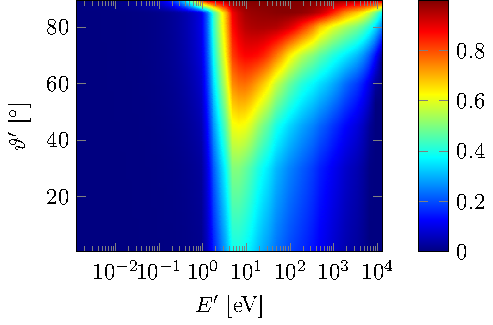
\includegraphics[width = 0.5\textwidth ]{Figures/RN.pdf}
	\caption{Particle reflection coefficient for deuterium projectiles on a carbon target.}
	\label{fig:RN}
\end{figure}

It is harder to calculate the other moment reflection coefficients (elaborating the integrals of Eqs.~\eqref{eq:Rmpar}, \eqref{eq:Rmperp}, \eqref{eq:Rp}, \eqref{eq:Rnn}, \eqref{eq:Rwwn}, and \eqref{eq:RE}) due to the specific format of the TRIM tables. Therefore, we use a Monte Carlo simulation with a very large amount of particles. For every combination of $v_{i}'$ and $\vartheta_{j}'$, we interpolate or extrapolate the whole TRIM table (e.g., Fig.~\ref{fig:trim}). Then, we launch a particle with speed $v_{i}'$, polar angle $\vartheta_{j}'$ and zero azimuthal angle and use the Monte Carlo procedure of Section~\ref{sec:MCbc}. This leads to a reflected speed $v_{k}$, polar angle $\vartheta_{k}$ and azimuthal angle $\varphi_{k}$. The process is repeated for $N$ particles. The moment reflection coefficient is estimated as
\begin{equation}
\hat{R}_{\mu}(v_{i}',\vartheta_{j}') = R_{\mathrm{N}}(v_{i}',\vartheta_{j}') \frac{1}{\mu(v_{i}',\vartheta_{j}',0)} \frac{1}{N} \sum_{k=1}^{N} \mu(v_{k},\vartheta_{k},\varphi_{k}),
\end{equation}
with the hat on top of $R$ indicating that it is a Monte Carlo estimation, and $\mu(v,\vartheta,\varphi)$ the particular moment, e.g., $\mu(v,\vartheta,\varphi) = v \sin \vartheta \cos \varphi$ for the parallel momentum reflection coefficient.

Fig.~\ref{fig:Rmoment} shows the results for deuterium impinging on carbon boundary material. For every combination of $v_{i}'$ and $\vartheta_{j}'$, $N = 10^{5}$ particles are used. Most moment reflection coefficients behave similarly as the particle reflection coefficient (Fig.~\ref{fig:RN}), with peak values for large incident angles and increase of the maximum value for fixed $\vartheta'$ when $\vartheta'$ increases. This is different for the density reflection coefficient (Fig.~\ref{fig:Rmp2}) due to the $1/v$ scaling in Eq.~\eqref{eq:Rnn}.
\begin{figure}[H]
	\centering
	\subfloat[Parallel momentum $\hat{R}_{\mathrm{m},||}$.]{
		\centering
		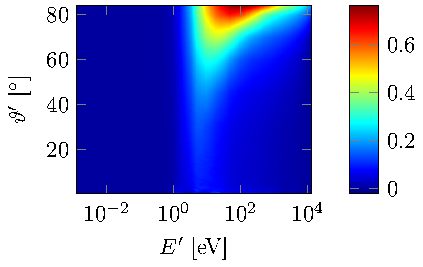
\includegraphics[width = 0.5\textwidth ]{Figures/Rmpar.pdf}
	}
	\subfloat[Perpendicular momentum $\hat{R}_{\mathrm{m},\perp}$.]{
		\centering
		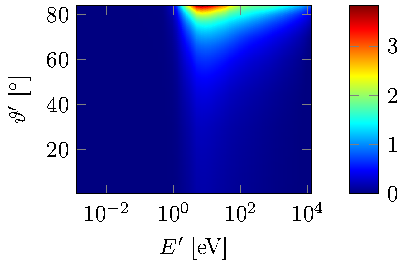
\includegraphics[width = 0.47\textwidth ]{Figures/Rmperp.pdf}
	} \\
	\subfloat[Pressure $\hat{R}_{p}$.]{
	\centering
	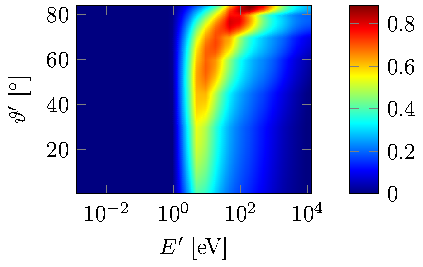
\includegraphics[width = 0.5\textwidth ]{Figures/Rmp1.pdf}
	}
	\subfloat[Density $\hat{R}_{\nn}$.]{
		\centering
		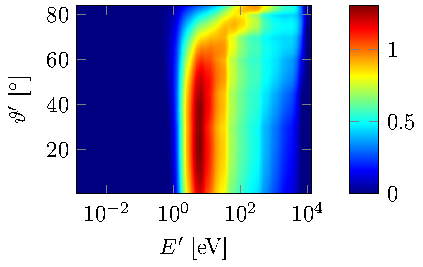
\includegraphics[width = 0.5\textwidth ]{Figures/Rmp2.pdf}
		\label{fig:Rmp2}
	} \\
	\subfloat[Toroidal velocity $\hat{R}_{\wwn}$.]{
	\centering
	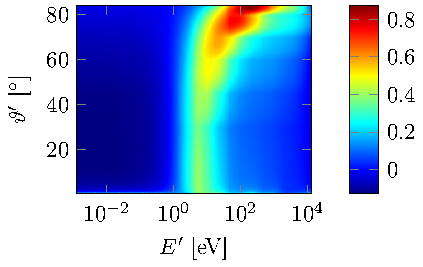
\includegraphics[width = 0.5\textwidth ]{Figures/Rmp3.pdf}
	}
	\subfloat[Energy $\hat{R}_{E}$.]{
		\centering
		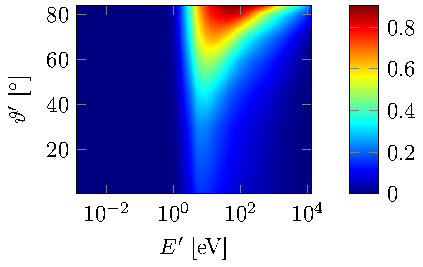
\includegraphics[width = 0.5\textwidth ]{Figures/RE.pdf}
	}
	\caption[TRIM moment reflection coefficients for deuterium projectiles on a carbon target.]{TRIM moment reflection coefficients for deuterium projectiles on a carbon target calculated with a Monte Carlo simulation.}
	\label{fig:Rmoment}
\end{figure}

\subsubsection{Resulting fluid boundary fluxes}
% ------------------------------------------------

We have characterized the TRIM database with seven moment reflection coefficients. Now, the integrals of Section~\ref{sec:boundaryfluxes} have to be calculated.

For the contributions of the incident neutrals (subscript $\nu-$), this can be done analytically. This leads to the following (particle, parallel momentum, and energy flux densities):
\begin{align}
\Gamma_{\nu-}^{\mathrm{n,diff}} =& - \frac{\nni\rcxm}{\nni\rcxm + \nne \rion} \left( \nn M^\mathrm{i}_{\nu} - \frac{1}{\nni\rcxm + \nne\rion} \left( \ddx{\nn}{\tau} M^\mathrm{i}_{\tau\nu} + \ddx{\nn}{\nu} M^\mathrm{i}_{\nu\nu} \right) \right), \label{eq:Gammanin2} \\
% -----------------------------------------------------------------------------------
\Gamma_{\mathrm{m},||,\nu-}^{\mathrm{n,diff}} =& -m \frac{\nni\rcxm}{\nni\rcxm + \nne\rion} \Bigg( \nn \left( \pit \left( \sin \alpha_{\nu} M^\mathrm{i}_{\tau\nu} + \cos \alpha_{\nu} M^\mathrm{i}_{\nu\nu} \right) + \pitt M^\mathrm{i}_{\phi\nu} \right) \nonumber \\
&- \frac{1}{\nni\rcxm + \nne\rion} \left( \ddx{\nn}{\tau} \left( \pit \left( \sin \alpha_{\nu} M^\mathrm{i}_{\tau\tau\nu} + \cos \alpha_{\nu} M^\mathrm{i}_{\tau\nu\nu} \right) + \pitt M^\mathrm{i}_{\phi\tau\nu} \right) \right. \nonumber \\
& \left. + \ddx{\nn}{\nu} \left( \pit \left( \sin \alpha_{\nu} M^\mathrm{i}_{\nu\nu\tau} + \cos \alpha_{\nu} \right) M^\mathrm{i}_{\nu\nu\nu} + \pitt M^\mathrm{i}_{\phi\nu\nu} \right) \right) \Bigg), \label{eq:Gammamompin} \\
% ----------------------------------------------------------------------------------
Q_{\nu-}^{\mathrm{n,diff}} =& -\frac{m}{2} \frac{\nni\rcxm}{\nni\rcxm + \nne\rion} \bigg ( \nn \left( M^\mathrm{i}_{\phi\phi\nu} + M^\mathrm{i}_{\tau\tau\nu} + M^\mathrm{i}_{\nu\nu\nu} \right) \nonumber \\
& - \frac{1}{\nni\rcxm + \nne \rion} \left( \ddx{\nn}{\tau} \left( M^\mathrm{i}_{\phi\phi\tau\nu} + M^\mathrm{i}_{\tau\tau\tau\nu} + M^\mathrm{i}_{\tau\nu\nu\nu} \right) \right. \nonumber \\
&\left. + \ddx{\nn}{\nu} \left( M^\mathrm{i}_{\phi\phi\nu\nu} + M^\mathrm{i}_{\tau\tau\nu\nu} + M^\mathrm{i}_{\nu\nu\nu\nu} \right) \right ) \bigg ), \label{eq:Qnin}
\end{align}
with
\begin{equation}
M^\mathrm{i}_{\alpha\beta\gamma\delta} = \int_{v_{\phi}'=-\infty}^{\infty} \int_{v_{\tau}'=-\infty}^{\infty} \int_{v_{\nu}' = - \infty}^{0} v_{\alpha}' v_{\beta}' v_{\gamma}' v_{\delta}' \widetilde{M}(v_{\phi}',v_{\tau}',v_{\nu}',\Vi,\Ti) \dd v_{\phi}' \dd v_{\tau}' \dd v_{\nu}',
\end{equation}

\noindent i.e., a certain moment of a Maxwellian distribution, with the subscripts indicating the particular velocity components by which the Maxwellian is multiplied. When using the drifting Maxwellian assumption instead of the diffusion assumption we get:

\begin{align}
\Gamma_{\nu-}^{\mathrm{n,Maxw}} =& - \nn M^\mathrm{n}_{\mathrm{n},\nu} ,   \label{eq:Gammanin2_maxw} \\
% -----------------------------------------------------------------------------------
\Gamma_{\mathrm{m},||,\nu-}^{\mathrm{n,Maxw}} =& -m \left( \nn \left( \pit \left( \sin \alpha_{\nu} M^\mathrm{n}_{\tau\nu} + \cos \alpha_{\nu} M^\mathrm{n}_{\nu\nu} \right) + \pitt M^\mathrm{n}_{\phi\nu} \right) \right), \label{eq:Gammamompin_maxw} \\
% ----------------------------------------------------------------------------------
Q_{\nu-}^{\mathrm{n,Maxw}} =& -\frac{m}{2} \left( \nn \left( M^\mathrm{n}_{\phi\phi\nu} + M^\mathrm{n}_{\tau\tau\nu} + M^\mathrm{n}_{\nu\nu\nu} \right) \right), \label{eq:Qnin_maxw}
\end{align}

with

\begin{equation}
M^\mathrm{n}_{\alpha\beta\gamma\delta} = \int_{v_{\phi}'=-\infty}^{\infty} \int_{v_{\tau}'=-\infty}^{\infty} \int_{v_{\nu}' = - \infty}^{0} v_{\alpha}' v_{\beta}' v_{\gamma}' v_{\delta}' \widetilde{M}(v_{\phi}',v_{\tau}',v_{\nu}',\Vn,\Tn) \dd v_{\phi}' \dd v_{\tau}' \dd v_{\nu}'\end{equation}

To obtain the fluid parallel momentum flux density of the incident neutrals $\Gamma_{\mathrm{m,f},||,\nu-}$, we have to subtract the pressure contribution from Eq.~\eqref{eq:Gammamompin}, as expressed by Eq.~\eqref{eq:Gammamompf}. Therefore, we also have to calculate the contributions from the incident neutrals to $\frac{m}{3} \int ||\vel||^{2} \frac{\Gamma^{\mathrm{n}}(\vel)}{|v_{\nu}|} \dd \vel$ (Eq.~\eqref{eq:v2fn}), $\nn'$ (Eq.~\eqref{eq:nnboundary}), and $\nn' \wwn'$ (Eq.~\eqref{eq:wwnboundary}). Elaborating these terms, gives for the diffusion approach
\begin{align}
\left [\frac{m}{3} \int ||\vel||^{2} \frac{\Gamma^{\mathrm{n}}(\vel)}{|v_{\nu}|} \dd \vel \right ]_{\nu-}^\mathrm{diff} =& \ \frac{m}{3} \frac{\nni\rcxm}{\nni\rcxm + \nne\rion} \bigg ( \nn \left( M_{\phi\phi}^\mathrm{i} + M_{\tau\tau}^\mathrm{i} + M_{\nu\nu}^\mathrm{i} \right) \nonumber \\
- & \frac{1}{\nni\rcxm + \nne\rion} \left( \ddx{\nn}{\tau} \left( M_{\phi\phi\tau}^\mathrm{i} + M_{\tau\tau\tau}^\mathrm{i} + M_{\nu\nu\tau}^\mathrm{i} \right) \right. \nonumber \\
+ & \left. \ddx{\nn}{\nu} \left( M_{\phi\phi\nu}^\mathrm{i} + M_{\tau\tau\nu}^\mathrm{i} + M_{\nu\nu\nu}^\mathrm{i} \right) \right) \bigg ), \label{eq:pnin} \\
% ------------------------------------------------------------------------------------------------
(n_{\mathrm{n},\nu-}')^\mathrm{diff} =& \ \frac{\nni\rcxm}{\nni\rcxm + \nne\rion} \bigg (\nn M^\mathrm{i} \nonumber \\
- & \frac{1}{\nni\rcxm + \nne\rion} \left (\ddx{\nn}{\tau} M^\mathrm{i}_{\tau} + \ddx{\nn}{\nu} M^\mathrm{i}_{\nu} \right ) \bigg ), \\
% ------------------------------------------------------------------------------------------------
\left [\nn'\wwn'\right ]_{\nu-}^\mathrm{diff} =& \ \frac{\nni\rcxm}{\nni\rcxm + \nne\rion} \bigg (\nn M_{\phi}^\mathrm{i} \nonumber \\
- & \frac{1}{\nni\rcxm + \nne\rion} \left (\ddx{\nn}{\tau} M_{\phi\tau}^\mathrm{i} + \ddx{\nn}{\nu} M_{\phi\nu}^\mathrm{i} \right ) \bigg ). \label{eq:wwnin}
\end{align}

For the drifting Maxwellian approach this becomes

\begin{align}
\left[ \frac{m}{3} \int ||\vel||^{2} \frac{\Gamma^{\mathrm{n}}(\vel)}{|v_{\nu}|} \dd \vel \right]_{\nu-}^\mathrm{Maxw} =& \ \frac{m}{3} \left( \nn \left( M_{\phi\phi}^\mathrm{n} + M_{\tau\tau}^\mathrm{n} + M_{\nu\nu}^\mathrm{n} \right) \right), \label{eq:pnin_maxw} \\
% ------------------------------------------------------------------------------------------------
(n_{\mathrm{n},\nu-}')^\mathrm{Maxw} =& \ \nn M^\mathrm{n}  \\
% ------------------------------------------------------------------------------------------------
\left [\nn'\wwn'\right ]_{\nu-}^\mathrm{Maxw} =& \ \nn M_{\phi}^\mathrm{n}. \label{eq:wwnin_maxw}
\end{align}

For the fast recycled and reflected contributions, the integrals can no longer be calculated analytically and they are evaluated numerically. To avoid the cost of recalculating the integrals every time the plasma state changes, the integrals are evaluated in advance for different values of the influencing plasma parameters. Every boundary flux density $\Gamma_{\mu}^{\mathrm{n}}$ of a particular moment $\mu$ can be written as
\begin{equation}
\Gamma_{\mu}^{\mathrm{n}} = \Gamma_{\mu,\nu-}^{\mathrm{n}} + \sum_{k}A_{\mu}^{k} \int_{v'=0}^{\infty} \int_{\vartheta'=0}^{\pi/2} \int_{\varphi'=0}^{2\pi} g_{\mu}^{k}(v',\vartheta',\varphi';{\bf R}) \fanorm(v',\vartheta',\varphi';\delta_{\mathrm{sh}}^{\mathrm{pot},k},\mathbf{V}_a,T_a) \dd v'\dd \vartheta' \dd \varphi', \label{eq:implementation}
\end{equation}
with $\Gamma_{\mu,\nu-}^{\mathrm{n}}$ the analytic expressions for the incident contributions (Eqs.~\eqref{eq:Gammanin2}-\eqref{eq:Qnin}, \eqref{eq:pnin}-\eqref{eq:wwnin}). The coefficient $A_{\mu}^{k}$ contains all terms that can be brought outside the integral (not functions of $v'$, $\vartheta'$, or $\varphi'$). The summation is used to distinguish between the different contributions. There is a contribution due to the recycled neutrals and three contributions of the reflected neutrals, respectively scaling with $\nn$, $\ddx{\nn}{\tau}$, and $\ddx{\nn}{\nu}$ (see Eq.~\eqref{eq:Gammanmin}). The integrand can be written as the product with a function $g_{\mu}^{k}(v',\vartheta',\varphi';{\bf R})$, which contains the needed TRIM reflection coefficients (present in ${\bf R}$). For the recycling contributions and the reflection contributions using the diffusion approximation, the Maxwellian distribution $\fanorm(v',\vartheta',\varphi';\delta_{\mathrm{sh}}^{\mathrm{pot},k},\mathbf{V}_a,T_a) \dd v'\dd \vartheta' \dd \varphi'$ is equal to the ion distribution $\finorm(v',\vartheta',\varphi';\delta_{\mathrm{sh}}^{\mathrm{pot},k},\Vi,\Ti)$ given by Eq.~\eqref{eq:finormdshpot}. The superscript $k$ for $\dshpot$ is needed to distinguish between the recycled and reflected neutrals. For the reflected neutrals using the diffusion approximation, $\delta_{\mathrm{sh}}^{\mathrm{pot},k} = 0$, whereas $\delta_{\mathrm{sh}}^{\mathrm{pot},k}$ is nonzero for the recycled neutrals if the boundary is not fully parallel to the magnetic field. For the reflected neutrals with the drifting Maxwellian assumption, $\fanorm(v',\vartheta',\varphi';\delta_{\mathrm{sh}}^{\mathrm{pot},k},\mathbf{V}_a,T_a) \dd v'\dd \vartheta' \dd \varphi'$ is equal to $\tilde{f}_\mathrm{n}(v',\vartheta',\varphi';0,\mathbf{V}_\mathrm{n},\Tn) \dd v'\dd \vartheta' \dd \varphi'$, given by Equation \eqref{eq:fnnorm}. Only the integral in Eq.~\eqref{eq:implementation} is calculated in advance and saved as a function of the sheath transmission coefficient, ion fluid velocity, and temperature:
\begin{equation}
\mathrm{RC}_{\mu}^{k}(\mathbf{V}_a,T_a) = \int_{v'=0}^{\infty} \int_{\vartheta'=0}^{\pi/2} \int_{\varphi'=0}^{2\pi} g_{\mu}^{k}(v',\vartheta',\varphi';{\bf R}) \fanorm(v',\vartheta',\varphi';\delta_{\mathrm{sh}}^{\mathrm{pot},k},\mathbf{V}_a,T_a) \dd v' \dd \vartheta' \dd \varphi'. \label{eq:Imu}
\end{equation}

To reduce the number of dependencies of $\mathrm{RC}_{\mu}^{k}$, we assume that $\mathbf{V}_a \approx \begin{bmatrix} u_{a,\phi} & 0 & 0 \end{bmatrix}^{T}$, expressed in the $(\phi,\tau,\nu)$ coordinate system. This assumption is valid for the ions if the pitch is sufficiently small such that the parallel direction almost coincides with the toroidal direction, and drifts are not included. For the neutrals in the drifting Maxwellian approximation, or for the ions when drifts are included, this assumption is less accurate. Even so, good fluid-kinetic agreement was achieved for cases with drifts in Ref. \cite{psi_wim}. Studying the role of the perpendicular bulk velocities, and finding a way to include them without making the databases unacceptably large, is subject of future work.  We evaluate Eq.~\eqref{eq:Imu} for 100 values of the Mach number $\mathcal{M}_{a,\phi} = u_{a,\phi}/\sqrt{2 T_a /m}$, uniformly distributed between 0 and 1.1 and 100 values for the temperature logarithmically distributed between 0.1 and 1\,000~eV. The midpoint integration rule is used with the discretized speed and polar angle from respectively Eq.~\eqref{eq:vdisc} and Eq.~\eqref{eq:thetadisc}, and the azimuthal angle $\varphi'$ discretized as
\begin{equation}
\varphi_{l}' = \frac{\pi}{400} + (l-1) \frac{\pi}{200}, \quad \text{for} \quad l = 1,\ldots, 400.
\end{equation}
Now, all integrated reflection coefficients are tabulated as a function of $\mathcal{M}_{a,\phi}$, $T_{a}$, and $\dshpot$.  During the simulation, we use linear interpolation for intermediate values of $\mathcal{M}_{a,\phi}$, $T_a$, and $\dshpot$.








\chapter{Implementation in SOLPS-ITER}

\section{Final expressions for macroscopic AFN database coefficients}\label{sec:final_expressions_RC}

The final expressions for the pre-computed integrals, as calculated in \texttt{CalcReflectionCoefficientsFluidTRIM}, are given here. In general, there are four coefficients per TRIM reflection coefficient.
There is a contribution due to the recycled neutrals and three contributions of the reflected neutrals, respectively scaling with $\nn$, $\dnndy$, and $\dnndz$ (see Eq.~\eqref{eq:Gammanmin}). However, the reflection term scaling with $\nn$ leads to the same integral as the recycling term scaling with $\nni$. These coefficients are called $\rconei$, $\rmxonei$, $\rmzonei$, $\rponeonei$, $\rptwoonei$, $\rpthreeonei$, and $\reonei$. The terms scaling with $\dnndy$ are often zero because $\int_{\varphi'=0}^{2 \pi} \mathrm{A} \sin(\varphi') \exp \left( \mathrm{B} + \mathrm{C} \cos(\varphi') \right) \dd \mathrm{\varphi'} = 0$. The exception is the tangential momentum components, where both the terms scaling with $\nn$ and $\dnndz$ are zero and only the $\dnndy$ term remains. The non-zero coefficients scaling with a neutral density gradient are $\rctwoi$, $\rmxtwoi$, $\rmytwoi$, $\rmztwoi$, $\rponetwoi$, $\rptwotwoi$, $\rpthreetwoi$, and $\retwoi$. The coefficients which are zero and hence not tabulated are $\mathrm{RC}_n^{\dnndy}$, $\mathrm{RC}_{\mathrm{m},\phi}^{\dnndy}$, $\mathrm{RC}_{\mathrm{m},\nu}^{\dnndy}$, $\mathrm{R}_{\mathrm{m},\tau}$, $\mathrm{RC}_{\mathrm{m},\tau}^{\dnndz}$, $\mathrm{RC}_{p}^{\dnndy}$, $\mathrm{RC}_{n_{\mathrm{n}}}^{\dnndy}$, $\mathrm{RC}_{u_{\mathrm{n},\phi}}^{\dnndy}$, and $\mathrm{RC}_{E}^{\dnndz}$.

%, where $\mathrm{A}$, $\mathrm{B}$, and $\mathrm{C}$ are coefficients that may depend on $v'$ and $\vartheta'$ but not on $\varphi'$.

The coefficients below are written as a function of $u_{a,\phi}$ and $T_a$. When evaluating the coefficients in \texttt{CalcRecycledFluxes} and \texttt{CalcReflectedFluxesDiffusion}, $a = \mathrm{i}$. When evaluating the coefficients in \texttt{CalcReflectedFluxesMaxwellian}, $a = \mathrm{n}$. Only for the recycling contributions is $\dshpot$ nonzero.

The term $\left( \frac{m}{2 \pi T_a} \right)^{\frac{3}{2}}$ in front of the exponential in the (sheath-accelerated) Maxwellian is rewritten as $\pi^{-\frac{3}{2}} \ca^{-3}$, where $\ca$ is the isothermal sound speed of species $a$. The coefficients are further divided by powers of $\ca$ to make them dimensionless, i.e. of the form
\begin{equation}
\mathrm{RC} = \frac{1}{\pi^{\frac{3}{2}}} \frac{1}{\ca^{k} }\int_{v'=0}^{\infty} \int_{\vartheta'=0}^{\pi/2} \int_{\varphi'=0}^{2\pi} R \ (v')^{k-1} F(\vartheta') G(\varphi') \dd v' \dd \vartheta' \dd \varphi'.
\end{equation}

The sheath acceleration is determined by $\Delta \phi_{\mathrm{sh}} = \dshpot ( \Te/ e )$, while the macroscopic reflection coefficients are tabulated as a function of $T_{\mathrm{i/n}}$. This is solved by evaluating the database for
\begin{equation}
\dshpotj = \dshpot \frac{T_{\mathrm{e}}}{T_{\mathrm{i/n}}} = \frac{\Delta \phi_{\mathrm{sh}} e}{T_{\mathrm{i/n}}}.
\end{equation}

A final point is that the reflection coefficients scaling with $\dnndz$ or $\dnndy$ will always be evaluated for $\dshpot = \dshpotj = 0$. However, they are currently also tabulated as a function of $\dshpot$ such that all coefficients have the same dimension.

\subsection{Macroscopic particle reflection coefficients}

\noindent Equations~\eqref{eq:Gammarefl}, \eqref{eq:Gammarec}, \eqref{eq:finorm}, and \eqref{eq:Gammanmin} lead to the definition of the macroscopic particle reflection coefficient scaling with density
\begin{align}
   \rconei & (u_{a,\phi},T_a,\dshpot) = \frac{1}{\pi^\frac{3}{2}} \frac{1}{\ca^4} \int_{v'=0}^{\infty} \int_{\vartheta'=0}^{\pi/2} \int_{\varphi'=0}^{2\pi}
    \Rv (v')^3 \times \nonumber \\
    \times & \exp \left( - \frac{m}{2 T_a} \left( (v')^2-2 (v') u_{a,\phi} \sin (\vartheta') \cos(\varphi') + u_{a,\phi}^2 - \frac{2 \dshpot T_a}{m} \right) \right) \cos (\vartheta') \sin (\vartheta')
    \dd v' \dd \vartheta' \dd \varphi', \label{eq:rconei_def}
\end{align}

\noindent and the macroscopic particle reflection coefficient scaling with the normal gradient of the neutral density

\begin{align}
    \rctwoi & (u_{a,\phi},T_a,\dshpot) =
     \frac{1}{\pi^{\frac{3}{2}}} \frac{1}{\ca^{5}} \int_{v'=0}^{\infty} \int_{\vartheta'=0}^{\pi/2} \int_{\varphi'=0}^{2\pi}
    \Rv (v')^4 \times \nonumber \\
    \times & \exp \left( - \frac{m}{2 T_a} \left( (v')^2-2 (v') u_{a,\phi} \sin (\vartheta') \cos (\varphi') + u_{a,\phi}^2 - \frac{2 \dshpot T_a}{m} \right) \right) \cos (\vartheta')^2 \sin (\vartheta')
    \dd v' \dd \vartheta' \dd \varphi'. \label{eq:rctwoi_def}
\end{align}

\noindent The macroscopic particle reflection coefficient scaling with the tangential gradient of the neutral density is zero and hence not tabulated:

\begin{align}
    \mathrm{RC}_n^{\dnndy} & (u_{a,\phi},T_a,\dshpot) =
     \frac{1}{\pi^{\frac{3}{2}}} \frac{1}{\ca^{5} }\int_{v'=0}^{\infty} \int_{\vartheta'=0}^{\pi/2} \int_{\varphi'=0}^{2\pi}
    \Rv (v')^4 \times \nonumber \\
    \times & \exp \left( - \frac{m}{2 T_a} \left( (v')^2-2 (v') u_{a,\phi} \sin (\vartheta') \cos (\varphi') + u_{a,\phi}^2 - \frac{2 \dshpot T_a}{m} \right) \right) \cos (\vartheta') \sin (\vartheta')^2 \sin (\varphi')
    \dd v' \dd \vartheta' \dd \varphi' = 0.
\end{align}

\subsection{Macroscopic momentum reflection coefficients}

Equations~\eqref{eq:finorm}, \eqref{eq:Gammanmin}, and the term in Eq.~\eqref{eq:Gammanmomp} that scales with $\pitt$ lead to the definition of the macroscopic toroidal momentum reflection coefficient scaling with density:

\begin{align}
    \rmxonei & (u_{a,\phi},T_a,\dshpot) =
         \frac{1}{\pi^\frac{3}{2}} \frac{1}{\ca^5} \int_{v'=0}^{\infty} \int_{\vartheta'=0}^{\pi/2} \int_{\varphi'=0}^{2\pi}
    \Rmomparv (v')^4 \times \nonumber \\
    \times & \exp \left( - \frac{m}{2 T_a} \left( (v')^2-2 (v') u_{a,\phi} \sin (\vartheta') \cos (\varphi') + u_{a,\phi}^2 - \frac{2 \dshpot T_a}{m} \right) \right) \cos (\vartheta') \sin (\vartheta')^2 \cos (\varphi')
    \dd v' \dd \vartheta' \dd \varphi', \label{eq:rmxonei_def}
\end{align}

\noindent and the macroscopic toroidal momentum reflection coefficient scaling with the normal gradient of neutral density
\begin{align}
    \rmxtwoi & (u_{a,\phi},T_a,\dshpot) =
    \frac{1}{\pi^\frac{3}{2}} \frac{1}{\ca^6} \int_{v'=0}^{\infty} \int_{\vartheta'=0}^{\pi/2} \int_{\varphi'=0}^{2\pi}
    \Rmomparv (v')^5 \times \nonumber \\
    \times & \exp \left( - \frac{m}{2 T_a} \left( (v')^2-2 (v') u_{a,\phi} \sin (\vartheta') \cos (\varphi') + u_{a,\phi}^2 - \frac{2 \dshpot T_a}{m} \right) \right) \left( \cos (\vartheta') \sin (\vartheta') \right)^2 \cos (\varphi')
    \dd v' \dd \vartheta' \dd \varphi'. \label{eq:rmxtwoi_def}
\end{align}

\noindent The macroscopic toroidal momentum reflection coefficient scaling with the tangential gradient of neutral density is zero and hence not tabulated:

\begin{align}
     \mathrm{RC}_{m,\phi}^{\dnndy} & (u_{a,\phi},T_a,\dshpot) =
    \frac{1}{\pi^\frac{3}{2}} \frac{1}{\ca^6} \int_{v'=0}^{\infty} \int_{\vartheta'=0}^{\pi/2} \int_{\varphi'=0}^{2\pi}
    \Rmomparv (v')^5 \times \nonumber \\
    \times & \exp \left( - \frac{m}{2 T_a} \left( (v')^2-2 (v') u_{a,\phi} \sin (\vartheta') \cos (\varphi') + u_{a,\phi}^2 - \frac{2 \dshpot T_a}{m} \right) \right) \cos (\vartheta') \sin (\vartheta')^3 \cos (\varphi') \sin (\varphi')
    \dd v' \dd \vartheta' \dd \varphi' = 0.
\end{align}

\noindent Equations~\eqref{eq:finorm}, \eqref{eq:Gammanmin}, and the term in Eq.~\eqref{eq:Gammanmomp} that scales with $\pit \sina$ lead to the definition of the macroscopic tangential momentum reflection coefficients. Now, the part scaling with density is zero:

\begin{align}
    \mathrm{R}_{\mathrm{m},\tau} & (u_{a,\phi},T_a,\dshpot) =
         \frac{1}{\pi^\frac{3}{2}} \frac{1}{\ca^5} \int_{v'=0}^{\infty} \int_{\vartheta'=0}^{\pi/2} \int_{\varphi'=0}^{2\pi}
    \Rmomparv (v')^4 \times \nonumber \\
    \times & \exp \left( - \frac{m}{2 T_a} \left( (v')^2-2 (v') u_{a,\phi} \sin (\vartheta') \cos (\varphi') + u_{a,\phi}^2 - \frac{2 \dshpot T_a}{m} \right) \right) \cos (\vartheta') \sin (\vartheta')^2 \sin (\varphi')
    \dd v' \dd \vartheta' \dd \varphi' = 0.
\end{align}

\noindent Also the part scaling with the normal gradient of neutral density is zero:

\begin{align}
    \mathrm{R}_{\mathrm{m},\tau} & (u_{a,\phi},T_a,\dshpot) =
         \frac{1}{\pi^\frac{3}{2}} \frac{1}{\ca^5} \int_{v'=0}^{\infty} \int_{\vartheta'=0}^{\pi/2} \int_{\varphi'=0}^{2\pi}
    \Rmomparv (v')^4 \times \nonumber \\
    \times & \exp \left( - \frac{m}{2 T_a} \left( (v')^2-2 (v') u_{a,\phi} \sin (\vartheta') \cos (\varphi') + u_{a,\phi}^2 - \frac{2 \dshpot T_a}{m} \right) \right) \cos (\vartheta') \sin (\vartheta')^2 \sin (\varphi') \cos (\varphi')
    \dd v' \dd \vartheta' \dd \varphi' = 0.
\end{align}

\noindent The macroscopic tangential momentum reflection coefficients scaling with the tangential gradient of neutral density is

\begin{align}
    \rmytwoi & (u_{a,\phi},T_a,\dshpot) =
      \frac{1}{\pi^\frac{3}{2}} \frac{1}{\ca^6} \int_{v'=0}^{\infty} \int_{\vartheta'=0}^{\pi/2} \int_{\varphi'=0}^{2\pi}
    \Rmomparv (v')^5 \times \nonumber \\
    \times & \exp \left( - \frac{m}{2 T_a} \left( (v')^2-2 (v') u_{a,\phi} \sin (\vartheta') \cos (\varphi') + u_{a,\phi}^2 - \frac{2 \dshpot T_a}{m} \right) \right) \cos (\vartheta') \sin (\vartheta')^3 \sin (\varphi')^2
    \dd v' \dd \vartheta' \dd \varphi'. \label{eq:rmytwo_def}
\end{align}

\noindent Equations~\eqref{eq:finorm}, \eqref{eq:Gammanmin}, and the term in Eq.~\eqref{eq:Gammanmomp} that scales with $\pit \cosa$ lead to the definition of the macroscopic normal momentum reflection coefficient scaling with density

\begin{align}
    \rmzonei & (u_{a,\phi},T_a,\dshpot) =
    \frac{1}{\pi^\frac{3}{2}} \frac{1}{\ca^5} \int_{v'=0}^{\infty} \int_{\vartheta'=0}^{\pi/2} \int_{\varphi'=0}^{2\pi}
    \Rmomperpv (v')^4 \times \nonumber \\
    \times & \exp \left( - \frac{m}{2 T_a} \left( (v')^2-2 (v') u_{a,\phi} \sin (\vartheta') \cos (\varphi') + u_{a,\phi}^2 - \frac{2 \dshpot T_a}{m} \right) \right) \cos (\vartheta')^2 \sin (\vartheta')
    \dd v' \dd \vartheta' \dd \varphi', \label{eq:rmzonei_def}
\end{align}

\noindent and the macroscopic normal momentum reflection coefficient scaling with the normal gradient of neutral density

\begin{align}
    \rmztwoi & (u_{a,\phi},T_a,\dshpot) =
        \frac{1}{\pi^\frac{3}{2}} \frac{1}{\ca^6} \int_{v'=0}^{\infty} \int_{\vartheta'=0}^{\pi/2} \int_{\varphi'=0}^{2\pi}
    \Rmomperpv (v')^5 \times \nonumber \\
    \times & \exp \left( - \frac{m}{2 T_a} \left( (v')^2-2 (v') u_{a,\phi} \sin (\vartheta') \cos (\varphi') + u_{a,\phi}^2 - \frac{2 \dshpot T_a}{m} \right) \right) \cos (\vartheta')^3 \sin (\vartheta')
    \dd v' \dd \vartheta' \dd \varphi'. \label{eq:rmztwoi_def}
\end{align}

\noindent The macroscopic normal momentum reflection coefficient scaling with the tangential gradient of neutral density is zero and hence not tabulated:

\begin{align}
    \mathrm{RC}_{\mathrm{m},\nu}^{\dnndy} & (u_{a,\phi},T_a,\dshpot) =
        \frac{1}{\pi^\frac{3}{2}} \frac{1}{\ca^6} \int_{v'=0}^{\infty} \int_{\vartheta'=0}^{\pi/2} \int_{\varphi'=0}^{2\pi}
    \Rmomperpv (v')^5 \times \nonumber \\
    \times & \exp \left( - \frac{m}{2 T_a} \left( (v')^2-2 (v') u_{a,\phi} \sin (\vartheta') \cos (\varphi') + u_{a,\phi}^2 - \frac{2 \dshpot T_a}{m} \right) \right) \cos (\vartheta')^2 \sin (\vartheta')^2 \sin (\varphi')
    \dd v' \dd \vartheta' \dd \varphi' = 0.
\end{align}

\subsection{Pressure contributions}

Equations~\eqref{eq:Gammamompf}, \eqref{eq:pnboundary}, and \eqref{eq:pnboundary2} introduce the need for additional coefficients to calculate the pressure of the fast reflected and recycled neutrals.

Equations~\eqref{eq:v2fn}, \eqref{eq:Gammanmin}, and \eqref{eq:finorm} lead to the definition of the part of the macroscopic pressure reflection coefficient scaling with density

\begin{align}
    \rponeonei & (u_{a,\phi},T_a,\dshpot) =
        \frac{1}{\pi^\frac{3}{2}} \frac{1}{\ca^5} \int_{v'=0}^{\infty} \int_{\vartheta'=0}^{\pi/2} \int_{\varphi'=0}^{2\pi}
    \Rpvone (v')^4 \times \nonumber \\
    \times & \exp \left( - \frac{m}{2 T_a} \left( (v')^2-2 (v') u_{a,\phi} \sin (\vartheta') \cos (\varphi') + u_{a,\phi}^2 - \frac{2 \dshpot T_a}{m} \right) \right) \sin (\vartheta')
    \dd v' \dd \vartheta' \dd \varphi', \label{eq:rponeonei_def}
\end{align}

\noindent and the part of the macroscopic pressure reflection coefficient scaling with the normal gradient of the neutral density

\begin{align}
    \rponetwoi & (u_{a,\phi},T_a,\dshpot) =
    \frac{1}{\pi^\frac{3}{2}} \frac{1}{\ca^6} \int_{v'=0}^{\infty} \int_{\vartheta'=0}^{\pi/2} \int_{\varphi'=0}^{2\pi}
    \Rpvone (v')^5 \times \nonumber \\
    \times & \exp \left( - \frac{m}{2 T_a} \left( (v')^2-2 (v') u_{a,\phi} \sin (\vartheta') \cos (\varphi') + u_{a,\phi}^2 - \frac{2 \dshpot T_a}{m} \right) \right)  \cos (\vartheta') \sin (\vartheta')
    \dd v' \dd \vartheta' \dd \varphi'. \label{eq:rponetwoi_def}
\end{align}

\noindent The part of the macroscopic pressure reflection coefficient scaling with the tangential gradient of the neutral density is again zero:

\begin{align}
    \mathrm{RC}_{p}^{\dnndy} & (u_{a,\phi},T_a,\dshpot) =
    \frac{1}{\pi^\frac{3}{2}} \frac{1}{\ca^3} \int_{v'=0}^{\infty} \int_{\vartheta'=0}^{\pi/2} \int_{\varphi'=0}^{2\pi}
    \Rpvone (v')^2 \times \nonumber \\
    \times & \exp \left( - \frac{m}{2 T_a} \left( (v')^2-2 (v') u_{a,\phi} \sin (\vartheta') \cos (\varphi') + u_{a,\phi}^2 - \frac{2 \dshpot T_a}{m} \right) \right)  \sin (\vartheta')^2 \sin (\varphi')
    \dd v' \dd \vartheta' \dd \varphi' = 0.
\end{align}

\noindent Equations~\eqref{eq:nnboundary}, \eqref{eq:Gammanmin}, and \eqref{eq:finorm} lead to the definition of the part of the macroscopic density reflection coefficient scaling with density

\begin{align}
    \rptwoonei & (u_{a,\phi},T_a,\dshpot) =
    \frac{1}{\pi^\frac{3}{2}} \frac{1}{\ca^4} \int_{v'=0}^{\infty} \int_{\vartheta'=0}^{\pi/2} \int_{\varphi'=0}^{2\pi}
    \Rpvtwo (v')^3 \times \nonumber \\
    \times & \exp \left( - \frac{m}{2 T_a} \left( (v')^2-2 (v') u_{a,\phi} \sin (\vartheta') \cos (\varphi') + u_{a,\phi}^2 - \frac{2 \dshpot T_a}{m} \right) \right) \sin (\vartheta')
    \dd v' \dd \vartheta' \dd \varphi', \label{eq:rptwoonei_def}
\end{align}

\noindent and the part of the macroscopic density reflection coefficient scaling with the normal gradient of the neutral density:

\begin{align}
    \rptwotwoi & (u_{a,\phi},T_a,\dshpot) =
    \frac{1}{\pi^\frac{3}{2}} \frac{1}{\ca^4} \int_{v'=0}^{\infty} \int_{\vartheta'=0}^{\pi/2} \int_{\varphi'=0}^{2\pi}
    \Rpvtwo (v')^3 \times \nonumber \\
    \times & \exp \left( - \frac{m}{2 T_a} \left( (v')^2-2 (v') u_{a,\phi} \sin (\vartheta') \cos (\varphi') + u_{a,\phi}^2 - \frac{2 \dshpot T_a}{m} \right) \right) \cos (\vartheta') \sin (\vartheta')
    \dd v' \dd \vartheta' \dd \varphi'. \label{eq:rptwotwo_def}
\end{align}

\noindent The part of the macroscopic density reflection coefficient scaling with the tangential gradient of the neutral density is again zero:

\begin{align}
    \mathrm{RC}_{n_{\mathrm{n}}}^{\dnndy} & (u_{a,\phi},T_a,\dshpot) =
    \frac{1}{\pi^\frac{3}{2}} \frac{1}{\ca^4} \int_{v'=0}^{\infty} \int_{\vartheta'=0}^{\pi/2} \int_{\varphi'=0}^{2\pi}
    \Rpvtwo (v')^3 \times \nonumber \\
    \times & \exp \left( - \frac{m}{2 T_a} \left( (v')^2-2 (v') u_{a,\phi} \sin (\vartheta') \cos (\varphi') + u_{a,\phi}^2 - \frac{2 \dshpot T_a}{m} \right) \right) \sin (\vartheta')^2 \sin (\varphi')
    \dd v' \dd \vartheta' \dd \varphi' = 0.
\end{align}

\noindent Equations~\eqref{eq:wwnboundary}, \eqref{eq:Gammanmin}, and \eqref{eq:finorm} lead to the definition of part of the macroscopic toroidal velocity reflection coefficient scaling with density

\begin{align}
    \rpthreeonei & (u_{a,\phi},T_a,\dshpot) =
    \frac{1}{\pi^\frac{3}{2}} \frac{1}{\ca^4} \int_{v'=0}^{\infty} \int_{\vartheta'=0}^{\pi/2} \int_{\varphi'=0}^{2\pi}
    \Rpvthree (v')^3 \times \nonumber \\
    \times & \exp \left( - \frac{m}{2 T_a} \left( (v')^2-2 (v') u_{a,\phi} \sin (\vartheta') \cos (\varphi') + u_{a,\phi}^2 - \frac{2 \dshpot T_a}{m} \right) \right) \sin (\vartheta')^2 \cos (\varphi')
    \dd v' \dd \vartheta' \dd \varphi', \label{eq:rpthreeonei_def}
\end{align}

\noindent and the part of the macroscopic toroidal velocity reflection coefficient scaling with the normal gradient of neutral density:

\begin{align}
    \rpthreetwoi & (u_{a,\phi},T_a,\dshpot) =
    \frac{1}{\pi^\frac{3}{2}} \frac{1}{\ca^5} \int_{v'=0}^{\infty} \int_{\vartheta'=0}^{\pi/2} \int_{\varphi'=0}^{2\pi}
    \Rpvthree (v')^4 \times \nonumber \\
    \times & \exp \left( - \frac{m}{2 T_a} \left( (v')^2-2 (v') u_{a,\phi} \sin (\vartheta') \cos (\varphi') + u_{a,\phi}^2 - \frac{2 \dshpot T_a}{m} \right) \right) \cos (\vartheta') \sin (\vartheta')^2 \cos (\varphi')
    \dd v' \dd \vartheta' \dd \varphi'. \label{eq:rpthreetwo_def}
\end{align}

\noindent The part of the macroscopic toroidal velocity reflection coefficient scaling with the tangential gradient of neutral density is again zero:

\begin{align}
    \mathrm{RC}_{u_{\mathrm{n},\phi}}^{\dnndy} & (u_{a,\phi},T_a,\dshpot) =
    \frac{1}{\pi^\frac{3}{2}} \frac{1}{\ca^5} \int_{v'=0}^{\infty} \int_{\vartheta'=0}^{\pi/2} \int_{\varphi'=0}^{2\pi}
    \Rpvthree (v')^4 \times \nonumber \\
    \times & \exp \left( - \frac{m}{2 T_a} \left( (v')^2-2 (v') u_{a,\phi} \sin (\vartheta') \cos (\varphi') + u_{a,\phi}^2 - \frac{2 \dshpot T_a}{m} \right) \right) \cos (\vartheta') \sin (\vartheta')^3 \sin (\varphi')
    \dd v' \dd \vartheta' \dd \varphi' = 0.
\end{align}

\subsection{Macroscopic neutral energy reflection coefficients}

Equations~\eqref{eq:Qnboundary}, \eqref{eq:Gammanmin}, and \eqref{eq:finorm} lead to the definition of the macroscopic energy reflection coefficient scaling with density

\begin{align}
    \reonei & (u_{a,\phi},T_a,\dshpot) =
            \frac{1}{\pi^\frac{3}{2}} \frac{1}{\ca^6} \int_{v'=0}^{\infty} \int_{\vartheta'=0}^{\pi/2} \int_{\varphi'=0}^{2\pi}
    \Rev (v')^5 \times \nonumber \\
    \times & \exp \left( - \frac{m}{2 T_a} \left( (v')^2-2 (v') u_{a,\phi} \sin (\vartheta') \cos (\varphi') + u_{a,\phi}^2 - \frac{2 \dshpot T_a}{m} \right) \right) \cos (\vartheta')^2 \sin (\vartheta')
    \dd v' \dd \vartheta' \dd \varphi', \label{eq:reonei_def}
\end{align}

and the macroscopic energy reflection coefficient scaling with the normal gradient of the neutral density

\begin{align}
    \retwoi & (u_{a,\phi},T_a,\dshpot) =
    \frac{1}{\pi^\frac{3}{2}} \frac{1}{\ca^7} \int_{v'=0}^{\infty} \int_{\vartheta'=0}^{\pi/2} \int_{\varphi'=0}^{2\pi}
    \Rev (v')^6 \times \nonumber \\
    \times & \exp \left( - \frac{m}{2 T_a} \left( (v')^2-2 (v') u_{a,\phi} \sin (\vartheta') \cos (\varphi') + u_{a,\phi}^2 - \frac{2 \dshpot T_a}{m} \right) \right) \cos (\vartheta')^2 \sin (\vartheta')
    \dd v' \dd \vartheta' \dd \varphi'. \label{eq:retwoi_def}
\end{align}

The macroscopic energy reflection coefficient scaling with the tangential gradient of the neutral density is zero:

\begin{align}
    \mathrm{RC}_{E}^{\dnndy} & (u_{a,\phi},T_a,\dshpot) =
    \frac{1}{\pi^\frac{3}{2}} \frac{1}{\ca^7} \int_{v'=0}^{\infty} \int_{\vartheta'=0}^{\pi/2} \int_{\varphi'=0}^{2\pi}
    \Rev (v')^6 \times \nonumber \\
    \times & \exp \left( - \frac{m}{2 T_a} \left( (v')^2-2 (v') u_{a,\phi} \sin (\vartheta') \cos (\varphi') + u_{a,\phi}^2 - \frac{2 \dshpot T_a}{m} \right) \right) \cos (\vartheta') \sin (\vartheta')^2 \sin (\varphi')
    \dd v' \dd \vartheta' \dd \varphi' = 0.
\end{align}

\section{Final expressions for net boundary fluxes}

Here, we re-write the expressions from the previous chapter in a form that closest resembles how they are implemented in the code. Recurring steps are:

\begin{itemize}
    \item The moments of the thermally released part $\Gamma_{\mu,\mathrm{T}}^{\mathrm{n,diff/Maxw}}$ is split into $\Gamma_{\mathrm{\mu,T,refl}}^{\mathrm{n,diff/Maxw}} + \Gamma_{\mathrm{\mu,T,rec}}^{\mathrm{n,diff/Maxw}}$, where $\Gamma_{\mathrm{\mu,T,refl}}^{\mathrm{n,diff/Maxw}}$ corresponds to the thermally released atoms originating from incident atoms, and $\Gamma_{\mathrm{\mu,T,rec}}^{\mathrm{n,diff/Maxw}}$ corresponds to the thermally released atoms originating from incident ions.
    \item The recycled parts are multiplied with $\frac{\fdni}{-\ionel}$. This is related to the factor $C^{\mathrm{i}}$ introduced in Equation~\eqref{eq:truncMaxw}. It compensates for the fact that integrating the assumed ion velocity distribution (that was used to determine the macroscopic fast recycling coefficients) can lead to a slightly different result than the macroscopic target ion flux in the fluid plasma solver.
    \item $\Ri$ and $\Rnx$ are replaced by $\pcorfi$ and $\pcorfn$, respectively, as explained in Section \ref{sec:pumped_fraction}.
\end{itemize}

\subsection{Net neutral particle flux density}

\noindent The net neutral particle flux density  $\Gamma^{\mathrm{n}} = \nn \Vn \cdot \Nu$ is written as

\begin{equation}
\Gamma^{\mathrm{n}} = \Gamma_{\mathrm{refl},\mathrm{F}}^{\mathrm{n,diff/Maxw}} + \Gamma_{\mathrm{rec},\mathrm{F}}^{\mathrm{n}} + \Gamma_{\mathrm{T,refl}}^{\mathrm{n,diff/Maxw}} +
\Gamma_{\mathrm{T,rec}}^{\mathrm{n,diff/Maxw}} - \Gamma_{\nu-}^{\mathrm{n,diff/Maxw}}.
\end{equation}\label{eq:net_particle_flux}

Here, $\Gamma_{\nu-}^{\mathrm{n,diff}}$ and $\Gamma_{\nu-}^{\mathrm{n,Maxw}}$ were already given as Eqs.~\eqref{eq:Gammanin2} and \eqref{eq:Gammanin2_maxw}. They are implemented in \texttt{CalcIncidentFluxesDiffusion} and \texttt{CalcIncidentFluxesMaxwellian}, respectively. For the recycled flux we have
\begin{equation}
\Gamma_{\mathrm{rec},\mathrm{f}} + \Gamma_{\mathrm{T,rec}}^{\mathrm{n}} = \Rifl (\Vi \cdot \boldsymbol{\nu}),
\end{equation}
as calculated in \texttt{CalcRecycledFluxes}. For the reflected fluxes we have
\begin{equation}
    \Gamma_{\mathrm{refl},\mathrm{f}}^{\mathrm{n,diff}} + \Gamma_{\mathrm{T}}^{\mathrm{n,diff}} = \Rnxfl \Gamma_{\nu-}^{\mathrm{n,diff}}
\end{equation}
as implemented \texttt{CalcReflectedFluxesDiffusion} or
\begin{equation}
        \Gamma_{\mathrm{refl},\mathrm{f}}^{\mathrm{n,Maxw}} +
        \Gamma_{\mathrm{T}}^{\mathrm{n,Maxw}} =
        \Rnxfl \Gamma_{\nu-}^{\mathrm{n,Maxw}}
\end{equation}

\noindent as implemented in \texttt{CalcReflectedFluxesMaxwellian}.

\subsection{Net neutral parallel momentum flux density}

The net neutral parallel momentum flux given by Equations~\eqref{eq:Gammamompf}, \eqref{eq:Gammanmomp}, and \eqref{eq:par_momentum_T} is finally implemented as

\begin{align}
\Gamma^{\mathrm{n,diff/Maxw}}_{\mathrm{m,||,f}} = & \ \Gamma^{\mathrm{n}}_{\mathrm{m,||,rec}} + \Gamma^{\mathrm{n,diff/Maxw}}_{\mathrm{m,||,refl}} +
\Gamma^{\mathrm{n,diff/Maxw}}_{\mathrm{m,||,T,rec}} +
\Gamma^{\mathrm{n,diff/Maxw}}_{\mathrm{m,||,T,refl}} -
\Gamma^{\mathrm{n,diff/Maxw}}_{\mathrm{m,||,inc}} \nonumber \\
& -
\pit \cosa \left( p^{\mathrm{n,diff/Maxw}}_{\mathrm{1,rec}} + p^{\mathrm{n,diff/Maxw}}_{\mathrm{1,refl}} + p^{\mathrm{n}}_{\mathrm{1,T,rec}} +
p^{\mathrm{n,diff/Maxw}}_{\mathrm{1,T,refl}} -
p^{\mathrm{n,diff/Maxw}}_{\mathrm{1,T,inc}} + p_2 \right) \label{eq:par_mom_final}
\end{align}

The $p_1$ terms correspond to term (1) in Equation~\eqref{eq:pnboundary2}. The $p_2$ term correspond to term (2) in Equation~\eqref{eq:pnboundary2} and is further elaborated below.

\subsubsection{Flux contributions}

Using the definition of $\rmzonei$ (Eq.~\eqref{eq:rmzonei_def}) and $\rmxonei$ (Eq.~\eqref{eq:rmxonei_def}), the fast recycled part of Eq.~\eqref{eq:Gammanmomp} is written as
\begin{equation}
\Gamma^{\mathrm{n}}_{\mathrm{m,||,rec}} = \pit \left( \fmozrec \cosa - \fmoyrec \sina \right) - \pitt \fmoxrec
\end{equation}
with
\begin{align}
    \fmozrec & = \pcorfi \ m \rmzonei \ci^2 \frac{\fdni}{-\ionel}, \\
    \fmoyrec & = 0, \\
    \fmoxrec & = \pcorfi \ m \rmxonei \ci^2 \frac{\fdni}{-\ionel} ,
\end{align}

where $ \pcorfi = \frac{\min \left( \pfi, \Rifl \right)}{\pfi}$ with

\begin{equation}
    \pfi = \frac{\rconei \ci}{-\ionel}.
\end{equation}

Using the definition of $\rmzonei$ (Eq.~\eqref{eq:rmzonei_def}), $\rmztwoi$ (Eq.~\eqref{eq:rmztwoi_def}), $\rmytwoi$ (Eq.~\eqref{eq:rmytwo_def}), $\rmxonei$ (Eq.~\eqref{eq:rmxonei_def}), and $\rmxtwoi$ (Eq.~\eqref{eq:rmxtwoi_def}), the fast reflected part of Eq.~\eqref{eq:Gammanmomp} according to the diffusion approximation is written as
\begin{equation}
    \Gamma^{\mathrm{n,diff}}_{\mathrm{m,||,refl}} = \pit \left( \fmozrefld \cosa - \fmoyrefld \sina \right) - \pitt \fmoxrefld
\end{equation}
with
\begin{align}
    \fmozrefld & = \pcorfnd m \frac{\vcx}{\vtot} \left( \nn \rmzonei \ci^2 + \frac{1}{\vtot} \dnndz \rmztwoi \ci^3 \right),\\
    \fmoyrefld & = \pcorfnd m \frac{\vcx}{(\vtot)^2} \dnndy \rmytwoi \ci^3, \\
    \fmoxrefld & = \pcorfnd m \frac{\vcx}{\vtot} \left( \nn \rmxonei \ci^2 + \frac{1}{\vtot} \dnndz \rmxtwoi \ci^3 \right),
\end{align}

where $ \pcorfnd = \frac{\min \left( \pfnd, \Rnxfl \right)}{\pfnd}$ with

\begin{equation}
    \pfnd = \frac{\vcx}{\vtot} \left( \nn \rconei \ci + \frac{1}{\vtot}\dnndz \rctwoi \ci^2 \right) \frac{1}{\fnnid}.
\end{equation}

When using the drifting Maxwellian approximation, the fast reflected parallel momentum flux becomes
\begin{equation}
    \Gamma^{\mathrm{n,Maxw}}_{\mathrm{m,||,refl}} = \pit \left( \fmozreflm \cosa - \fmoyreflm \sina \right) - \pitt \fmoxreflm
\end{equation}

with
\begin{align}
    \fmozreflm & = \pcorfnm m \nn \rmzonei \cn^2, \\
    \fmoyreflm & = 0, \\
    \fmoxreflm & = \pcorfnm m \nn \rmxonei \cn^2.
\end{align}

where $ \pcorfnm = \frac{\min \left( \pfnm, \Rnxfl \right)}{\pfnm}$ with

\begin{equation}
    \pfnm = \frac{ \nn \rconei \cn}{\fnnim} .
\end{equation}

The thermally recycled contribution to the parallel momentum flux from Eq.~\eqref{eq:par_momentum_T} is written as

\begin{equation}
    \Gamma^{\mathrm{n}}_{\mathrm{m,||,T,rec}} = \pit \fmozrect \cosa
\end{equation}

%    \Gamma^{\mathrm{n}}_{\mathrm{m,||,T,rec}} = \pit \left( \fmozrect \cosa + \fmoyrect \sina \right) + \pitt \fmoxrect

with
\begin{align}
    \fmozrect & = \pti \frac{2}{3} m \fdni \vT,
%    \fmoyrect & = 0, \\
%    \fmoxrect & = 0.
\end{align}

where $\pti = \max \left( \Rifl - \pfi, 0 \right)$. \\

The thermally reflected contribution to the parallel momentum flux from Eq.~\eqref{eq:par_momentum_T} is written as

\begin{equation}
    \Gamma^{\mathrm{n,diff}}_{\mathrm{m,||,T,refl}} = \pit \fmozrefldt \cosa
\end{equation}
with
\begin{align}
    \fmozrefldt & = \ptnd \frac{2}{3} m \fnnid \vT
%    \fmoyrefldt & = 0, \\
%    \fmoxrefldt & = 0.
\end{align}

where $\ptnd = \max \left( \Rnxfl - \pfnd , 0 \right)$. When using the drifting Maxwellian assumption, this becomes

\begin{equation}
    \Gamma^{\mathrm{n,Maxw}}_{\mathrm{m,||,T,refl}} = \pit \fmozreflmt \cosa
\end{equation}

with
\begin{align}
    \fmozreflmt & = \ptnm \frac{2}{3} m \fnnim \vT.
%    \fmoyreflmt & = 0, \\
%    \fmoxreflmt & = 0.
\end{align}

The incident flux of parallel momentum according to the diffusion approximation (Eq.~\eqref{eq:Gammamompin}) is written as
\begin{equation}
    \Gamma^{\mathrm{n,diff}}_{\mathrm{m,||,inc}} = \pit \left( \fmozincd \cosa - \fmoyincd \sina \right) - \pitt \fmoxincd
\end{equation}

with
\begin{align}
    \fmozincd & = m \frac{\vcx}{\vtot} \left( - \nn \itwol + \frac{1}{\vtot} \left( \dnndy \uy \itwol + \dnndz \ithreel \right) \right), \\
    \fmoyincd & = m \frac{\vcx}{\vtot} \left( - \nn \uy \ionel + \frac{1}{\vtot} \left( \dnndy \left( \frac{\Ti}{m} + \uy^2 \right) \ionel + \dnndz \uy \itwol \right) \right),\\
    \fmoxincd & = m \frac{\vcx}{\vtot} \left( - \nn \ux \ionel + \frac{1}{\vtot} \left( \dnndy \ux \uy \ionel + \dnndz \ux \itwol \right) \right).
\end{align}

When using the drifting Maxwellian approximation, this becomes
\begin{equation}
    \Gamma^{\mathrm{n,Maxw}}_{\mathrm{m,||,inc}} =  -\pit \left( \fmozincm \cosa + \fmoyincm \sina \right) - \pitt \fmoxincm
\end{equation}

with
\begin{align}
    \fmozincm & = - m \nn \itwol, \\
    \fmoyincm & = - m \nn \uyn \ionel, \\
    \fmoxincm & = - m \nn \uxn \ionel.
\end{align}

\subsubsection{Term (1) pressure contributions}

Using the definition of $\rponeonei$ (Eq.~\eqref{eq:rponeonei_def}) and $\rponetwoi$ (Eq.~\eqref{eq:rponetwoi_def}), the term (1) pressure contributions from Equation~\eqref{eq:v2fn} as written in Eq.~\eqref{eq:par_mom_final} become
\begin{equation}
     p^{\mathrm{n}}_{\mathrm{1,rec}} = \pcorfi \frac{m}{3} \rponeonei \ci^2 \frac{\fdni}{-\ionel},
\end{equation}

\begin{equation}
    p^{\mathrm{n,diff}}_{\mathrm{1,refl}} = \pcorfnd \frac{m}{3} \frac{\vcx}{\vtot} \left( \nn + \rponeonei \ci^2 + \frac{1}{\vtot} \dnndz \rponetwoi \ci^3 \right),
\end{equation}

\begin{equation}
    p^{\mathrm{n,Maxw}}_{\mathrm{1,refl}} = \pcorfnm \frac{m}{3} \nn \rponeonei \cn^2,
\end{equation}

\begin{equation}
    p^{\mathrm{n}}_{\mathrm{1,T,rec}} = \pti \frac{2}{3} \ m \ \fdni \vT ,
\end{equation}

\begin{equation}
    p^{\mathrm{n,diff}}_{\mathrm{1,T,refl}} = \ptnd \frac{2}{3} \ m \ \fnnid \vT ,
\end{equation}

\begin{equation}
    p^{\mathrm{n,Maxw}}_{\mathrm{1,T,refl}} = \ptnm \frac{2}{3} \ m \ \fnnim \vT ,
\end{equation}

\begin{align}
    p^{\mathrm{n,diff}}_{\mathrm{1,inc}} & =
    \frac{m}{3} \frac{\vcx}{\vtot} \left( \nn \left( \left( \frac{2 \Ti}{m} + \ux^2 + \uy^2 \right) \izerol + \itwol \right) \right. \\ & \left. - \frac{1}{\vtot} \left( \dnndy \left( \left( \frac{4 \Ti}{m} \uy + \ux^2 \uy + \uy^3 \right) \izerol + \uy \itwol \right) + \dnndz \left( \left( \frac{2 \Ti}{m} + \ux^2 + \uy^2 \right) \ionel + \ithreel \right) \right) \right),
\end{align}

\begin{equation}
    p^{\mathrm{n,Maxw}}_{\mathrm{1,inc}} =
    \frac{m}{3} \left( \nn \left( \left( \frac{2 T_{\mathrm{n}}}{m} + \uxn^2 + \uyn^2 \right) \izerol + \itwol \right) \right).
\end{equation}

\subsubsection{Term (2) pressure contributions}

The contribution from Equation~\eqref{eq:pnboundary_term2} is implemented in the code as

\begin{align} \label{eq:p2_final}
    p_2 & = \frac{m}{3} \nn' \wwn'^{2} =  \frac{m}{3} \frac{(\nn' \wwn')^2}{\nn'} \nonumber \\
    & = \frac{m}{3} \frac{\left( (\nn' \wwn')_{\mathrm{rec}} + (\nn' \wwn')_{\mathrm{refl}}^{\mathrm{diff/Maxw}} + (\nn' \wwn')_{\mathrm{T,rec}} + (\nn' \wwn')_{\mathrm{T,refl}}^{\mathrm{diff/Maxw}} + (\nn' \wwn')_{\mathrm{inc}}^{\mathrm{diff/Maxw}} \right)^2}{\left( (\nn')_{\mathrm{rec}} + (\nn')_{\mathrm{refl}}^{\mathrm{diff/Maxw}} + (\nn')_{\mathrm{T,rec}} + (\nn')_{\mathrm{T,refl}}^{\mathrm{diff/Maxw}} + (\nn')_{\mathrm{inc}}^{\mathrm{diff/Maxw}} \right)}.
\end{align}

Using the definition of $\rptwoonei$ (Eq.~\eqref{eq:rptwoonei_def}) and $\rptwotwoi$ (Eq.~\eqref{eq:rptwotwo_def}), the density contributions from Eq.~\eqref{eq:nnboundary} as written in Eq.~\eqref{eq:p2_final} are given by

\begin{align}
    (\nn')_{\mathrm{rec}} & = \pcorfi \rptwoonei \frac{\fdni}{-\ionel}, \\
    %-------
    (\nn')_{\mathrm{refl}}^{\mathrm{diff}} & = \pcorfnd \frac{\vcx}{\vtot} \left( \nn \rptwoonei + \frac{1}{\vtot} \dnndz \rptwotwoi \ci \right), \\
    %-------
    (\nn')_{\mathrm{refl}}^{\mathrm{Maxw}} & = \pcorfnm \nn \rptwoonei, \\
    %-------
     (\nn')_{\mathrm{T,rec}} & = \pti \fdni \frac{2}{\vT}, \\
    %-------
    (\nn')_{\mathrm{T,refl}}^{\mathrm{diff}} & = \ptn \fnnid \frac{2}{\vT}, \\
    %-------
    (\nn')_{\mathrm{T,refl}}^{\mathrm{Maxw}} & = \ptn \fnnim \frac{2}{\vT}, \\
    %-------
    (\nn')_{\mathrm{inc}}^{\mathrm{diff}} & = \frac{\vcx}{\vtot} \left( \nn \izerol - \frac{1}{\vtot} \left( \dnndy \uy \izerol + \dnndz \ionel \right) \right), \\
    %-------
    (\nn')_{\mathrm{inc}}^{\mathrm{Maxw}} & = \nn \izerol. \\
    %-------
\end{align}

Using the definition of $\rpthreeonei$ (Eq.~\eqref{eq:rpthreeonei_def}) and $\rpthreetwoi$ (Eq.~\eqref{eq:rpthreetwo_def}), the $(\nn' \wwn')$ terms from Eq.~\eqref{eq:wwnboundary} as written in Eq.~\eqref{eq:p2_final} are written as
\begin{align}
    (\nn' \wwn')_{\mathrm{rec}} & = \pcorfi \rpthreeonei \ci \frac{\fdni}{-\ionel}, \\
    %-------
    (\nn' \wwn')_{\mathrm{refl}}^{\mathrm{diff}} & = \pcorfnd \frac{\vcx}{\vtot} \left( \nn \rpthreeonei \ci + \frac{1}{\vtot} \dnndz \rpthreetwoi \ci^2 \right), \\
    %-------
    (\nn' \wwn')_{\mathrm{refl}}^{\mathrm{Maxw}} & = \pcorfnm \nn \rpthreeonei \cn, \\
    %-------
    (\nn' \wwn')_{\mathrm{T,rec}} & = 0, \\
    %-------
    (\nn' \wwn')_{\mathrm{T,refl}}^{\mathrm{diff}} & = 0, \\
    %-------
    (\nn' \wwn')_{\mathrm{T,refl}}^{\mathrm{Maxw}} & = 0, \\
    %-------
    (\nn' \wwn')_{\mathrm{inc}}^{\mathrm{diff}} & = (\nn')_{\mathrm{inc}}^{\mathrm{diff}} \ux, \\
    %-------
    (\nn' \wwn')_{\mathrm{inc}}^{\mathrm{Maxw}} & = (\nn')_{\mathrm{inc}}^{\mathrm{Maxw}} \uxn.
\end{align}

\subsection{Net neutral energy flux density}

Similar to the particle and parallel momentum flux, we write the net neutral energy flux density given by Eqs.~\eqref{eq:Qnboundary} and \eqref{eq:Qnboundary_efc} as follows:

\begin{equation}
    Q^{\mathrm{n,diff/Maxw}} = Q^{\mathrm{n}}_{\mathrm{rec}} + Q^{\mathrm{n,diff/Maxw}}_{\mathrm{refl}} + Q^{\mathrm{n}}_{T,\mathrm{rec}} + Q^{\mathrm{n,diff/Maxw}}_{\mathrm{T,refl}} - Q^{\mathrm{n,diff/Maxw}}_{\mathrm{T,inc}}
\end{equation}

\noindent Using the definitions of $\reonei$ (Eq.~\eqref{eq:reonei_def}) and $\retwoi$ (Eq.~\eqref{eq:retwoi_def}), the components are written as

\begin{align}
    Q^{\mathrm{n}}_{\mathrm{rec}} & = \frac{1}{2} \pcorfi m \reonei \ci^3 \frac{\fdni}{-\ionel}, \\
    Q^{\mathrm{n,diff}}_{\mathrm{refl}} & = \frac{1}{2} \pcorfnd m \frac{\vcx}{\vtot} \left( - \nn \reonei \ci^3 + \frac{1}{\vtot} \dnndz \retwoi \ci^4 \right), \\
    Q^{\mathrm{n,Maxw}}_{\mathrm{refl}} & = \pcorfnm m \nn \reonei \cn^3, \\
    Q^{\mathrm{n}}_{\mathrm{T,rec}} & = \pti \fdni \efc, \\
    Q^{\mathrm{n,diff}}_{\mathrm{T,refl}} & = \ptn \fnnid \efc, \\
    Q^{\mathrm{n,Maxw}}_{\mathrm{T,refl}} & = \ptn \fnnim \efc,\\
    Q^{\mathrm{n,diff}}_{\mathrm{inc}} & = \frac{\vcx}{\vtot} \Bigg\{ -\nn \left( \left(\Ti + \frac{m}{2} \left( \ux^2 + \uy^2 \right) \right) \ionel + \frac{m}{2} \ithreel \right) \nonumber \\ & + \frac{1}{\vtot} \Bigg[ \dnndy \left( \left( 2 \Ti + \frac{m}{2} \left( \ux^2 + \uy^2 \right) \right) \uy \ionel + \frac{m}{2} \uy \ithreel \right) \nonumber \\
    & + \dnndz \left( \left( \Ti + \frac{m}{2} \left( \ux^2 + \uy^2 \right) \right) \itwol + \frac{m}{2} \ifourl \right) \Bigg] \Bigg\}, \\
    Q^{\mathrm{n,Maxw}}_{\mathrm{inc}} & = -\nn \left( \left( \Tn + \frac{m}{2} \left( \uxn^2 + \uyn^2 \right) \right) \ionel + \frac{m}{2} \ithreel \right).
\end{align}

\section{Link between symbols and code variables}

This section is specifically aimed at expert users of the AFN boundary conditions and future researchers that wish to improve them. It links the symbolic notation used in this document to the variable names in the code.

\subsection{Pre-processor b2ab}

\begin{tabular}{L{3cm} L{4cm}}
\underline{Symbol} & \underline{Code} \\
$m$ & \texttt{const.m}\\
$\mathbf{v}'$ & \texttt{vi}\\
$\mathbf{v}$ & \texttt{vo}\\
$\varphi$ & \texttt{phiR}\\
$\varphi'$ & \texttt{phi} \\
$\vartheta$ & \texttt{thetaR}\\
$\vartheta'$ & \texttt{thetai}\\
$c_a$ & \texttt{cs}\\
$\delta^{\mathrm{pot}}_{\mathrm{sh}}$ & \texttt{deltaP}\\
$T_{\mathrm{e}}$ & \texttt{te}\\
$T_{\mathrm{i}}$ & \texttt{ti}\\
$v_{\mathrm{min}}$ & \texttt{vmin}\\
$\vartheta_{\mathrm{max}}$ & \texttt{thetamax}\\
$\Rv$ & \texttt{TRIMRv} \\
$\Rmomparv$ & \texttt{TRIMRmomparv}\\
$\Rmomperpv$ & \texttt{TRIMRmomperpv}\\
$\Rpvone$ & \texttt{TRIMRpv1}\\
$\Rpvtwo$ & \texttt{TRIMRpv2}\\
$\Rpvthree$ & \texttt{TRIMRpv3}\\
$\Rev$ & \texttt{TRIMREv}\\
\end{tabular}

\subsection{Macroscopic reflection coefficients}

\begin{tabular}{L{2cm} L{6cm} L{4cm}}
\underline{Symbol} & \underline{in \texttt{b2mod\_create\_afn\_bc\_tables}} & \underline{in \texttt{b2mod\_recycle}} \\
$\rconei$ & \texttt{R1} & \texttt{rc1i} \\
$\rctwoi$ & \texttt{R2} & \texttt{rc2i} \\
$\rmxonei$ & \texttt{Rmx1} &  \texttt{rmx1i} \\
$\rmxtwoi$ & \texttt{Rmx2} & \texttt{rmx2i} \\
$\rmytwoi$ & \texttt{Rmy2} & \texttt{rmy2i} \\
$\rmzonei$ & \texttt{Rmz1} &  \texttt{rmz1i} \\
$\rmztwoi$ & \texttt{Rmz2} &  \texttt{rmz2i} \\
$\reonei$ & \texttt{RE1} & \texttt{re1i} \\
$\retwoi$ & \texttt{RE2} & \texttt{re2i} \\
$\rponeonei$ & \texttt{Rp11} & \texttt{rp11i} \\
$\rponetwoi$ & \texttt{Rp12} &  \texttt{rp12i} \\
$\rptwoonei$ & \texttt{Rp21} &  \texttt{rp21i} \\
$\rptwotwoi$ & \texttt{Rp22} & \texttt{rp22i} \\
$\rpthreeonei$ & \texttt{Rp31} & \texttt{rp31i} \\
$\rpthreetwoi$ & \texttt{Rp32} & \texttt{rp32i} \\
\end{tabular}


\subsection{Runtime}

\subsubsection{General}

\begin{tabular}{L{3cm} L{8cm}}
\underline{Symbol} & \underline{Code} \\
$e$ & \texttt{qe} \\
$\nn$ & \texttt{nnf} or \texttt{nn} \\
$\pit$ & \texttt{pit} \\
$\pitt$ & \texttt{pit2} \\
$\pfi$ or $\pfn$ &  \texttt{pf}\\
$\pcorfi$ or $\pcorfn$ &  \texttt{pcorf}\\
$\pti$ or $\ptn $ &  \texttt{pt}\\
$\Rnxfl$ or $\Rifl$ &  \texttt{recyc0} or \texttt{b2recyc} \\
$\recycm$ & \texttt{recycm}\\
$\cosa$ & \texttt{cosa} \\
$\sina$ & \texttt{sina} \\
$\phi$ & \texttt{x} \\
$\tau$ & \texttt{y} \\
$\nu$ & \texttt{z} \\
$u_{||}$ or $u_{\mathrm{n}||}$ & \texttt{upf} \\
$ \ux $ or $ \uxn $ & \texttt{ux} \\
$ \uy $ or $ \uyn$ & \texttt{uy} \\
$ \uz $ or $ \uzn $ & \texttt{uz} \\
$\mathcal{M}_\phi$ & \texttt{Mj}\\
$A_f$ & \texttt{area} \\
$\vcx$ & \texttt{vcx} \\
$\vion$ & \texttt{vion} \\
$\vtot$ & \texttt{vtot} \\
$v_{\mathrm{T}}$ & \texttt{vt}\\
$\Gamma^{\mathrm{n}}_H - Q^{\mathrm{n}}$ & \texttt{q\_conv}\\
$\Tn$ & \texttt{tf}\\
$\Ti$ & \texttt{tif}\\
$\vT$ & \texttt{vt}\\
$\efc$ & \texttt{E\_fc}\\
$\mathrm{Kn}$ & \texttt{Kn} \\
$L$ & \texttt{L} or \texttt{L\_macro\_AFN}  \\
$\mathrm{Kn^{bd}}$ & \texttt{Kn\_b1} \\
$\mathrm{Kn^{bm}}$ & \texttt{Kn\_b2} \\
$c_{\mathrm{n},th}$ & \texttt{c\_th} \\
$\ci $ or $ \cn $ & \texttt{cs} \\
$\lambda_{\mathrm{cx}}$ & \texttt{mfp} \\
$\dshpotj$ & \texttt{shpottauj}
\end{tabular}

\subsubsection{Moments of Maxwellian}
\begin{tabular}{L{3cm} L{8cm}}
\underline{Symbol} & \underline{Code} \\
$\izerol$ & \texttt{i0l} \\
$\ionel$ & \texttt{i1l} \\
$\itwol$ & \texttt{i2l} \\
$M_{\tau \nu}$ &  \texttt{uy*i1l} \\
$M_{\phi \nu}$ & \texttt{ux*i1l} \\
$M_{\tau \tau \nu}$ & \texttt{(ti/mn + uy**2)*i1l} \\
$M_{\tau \nu \nu}$ &  \texttt{uy*i2l}\\
$M_{\phi \tau \nu}$ &  \texttt{ux*uy*i1l}\\
$\ithreel$ &  \texttt{i3l}\\
$M_{\phi \nu \nu}$ &  \texttt{ux*i2l}\\
$M_{\phi \phi \nu}$ &  \texttt{(ti/mn + ux**2)*i1l}\\
$M_{\phi \phi \tau \nu}$ &  \texttt{(ti/mn + ux**2)*uy*i1l}\\
$M_{\tau \tau \tau \nu}$ &  \texttt{(ti/mn + uy**2)*uy*i1l}\\
$M_{\tau \nu \nu \nu}$ &  \texttt{uy*i3l}\\
$M_{\phi \phi \nu \nu}$ &  \texttt{(ti/mn + ux**2)*i2l}\\
$M_{\tau \tau \nu \nu}$ &  \texttt{(ti/mn + uy**2)*i2l} \\
$M_{\nu \nu \nu \nu}$ &  \texttt{i4l}\\
\end{tabular}

\subsubsection{CalcIncidentFluxesDiffusion/Maxwellian}

\begin{tabular}{L{4cm} L{6cm}}
\underline{Symbol} & \underline{Code} \\
$\fmoxincd $ or $ \fmoxincm$ & \texttt{fmox} \\
$\fmoyincd $ or $ \fmoyincm$ & \texttt{fmoy} \\
$\fmozincd $ or $ \fmozincm$ & \texttt{fmoz} \\
$ \Gamma^{\mathrm{n,diff}}_{\mathrm{m,||,inc}}$ or  $\Gamma^{\mathrm{n,Maxw}}_{\mathrm{m,||,inc}} $ & \texttt{fmomni} \\
$Q^{\mathrm{n,diff}}_{\mathrm{inc}} $ or  $ Q^{\mathrm{n,Maxw}}_{\mathrm{inc}}$ & \texttt{feneni} \\
$(\nn')_{\mathrm{inc}}^{\mathrm{diff}} $ or  $ (\nn')_{\mathrm{inc}}^{\mathrm{Maxw}}$ & \texttt{nni} \\
$ (\nn' \wwn')_{\mathrm{inc}}^{\mathrm{diff}}$ & \texttt{nnwwni} \\
$p^{\mathrm{n,diff}}_{\mathrm{1,inc}} $ or  $ p^{\mathrm{n,Maxw}}_{\mathrm{1,inc}}$ & \texttt{pn} \\
\end{tabular}

\subsubsection{CalcRecycledFluxes}

\begin{tabular}{L{5cm} L{8cm}}
\underline{Symbol} & \underline{Code} \\
$\fmoxrec$ & \texttt{fmox} \\
$\fmoyrec$ & \texttt{fmoy} \\
$\fmozrec + \fmozrect $ &  \texttt{fmoz} \\
$p^{\mathrm{n}}_{\mathrm{1,rec}} + p^{\mathrm{n}}_{\mathrm{1,T,rec}} $ & \texttt{pnc} \\
$(\nn')_{\mathrm{rec}} + (\nn')_{\mathrm{T,rec}}$ &  \texttt{nnrec} \\
$(\nn' \wwn')_{\mathrm{rec}}$ & \texttt{nnwwnrec} \\
$Q^{\mathrm{n}}_{\mathrm{rec}} + Q^{\mathrm{n}}_{\mathrm{T,rec}}$ & \texttt{fenec} \\
$\Gamma^{\mathrm{n}}_{\mathrm{m,||,rec}} + \Gamma^{\mathrm{n}}_{\mathrm{m,||,T,rec}}$ & \texttt{fmomrec} \\
\end{tabular}

\subsubsection{CalcReflectedFluxesDiffusion/Maxwellian}

\begin{tabular}{L{8cm} L{3cm}}
\underline{Symbol} & \underline{Code} \\
$\fmoxrefld $ or  $ \fmoxreflm$ & \texttt{fmox} \\
$\fmoyrefld $ or  $ \fmoyreflm$ & \texttt{fmoy} \\
$ \fmozrefld + \fmozrefldt$ or  $ \fmozreflm + \fmozreflmt $  & \texttt{fmoz} \\
$ (\nn')_{\mathrm{refl}}^{\mathrm{diff/Maxw}} + (\nn')_{\mathrm{T,refl}}^{\mathrm{diff/Maxw}} $& \texttt{nnrefl} \\
$(\nn' \wwn')_{\mathrm{refl}}^{\mathrm{diff/Maxw}}$ & \texttt{nnwwnrefl} \\
$Q^{\mathrm{n,diff/Maxw}}_{\mathrm{refl}} + Q^{\mathrm{n,diff/Maxw}}_{\mathrm{T,refl}}$ & \texttt{fene} \\
$\Gamma^{\mathrm{n,diff/Maxw}}_{\mathrm{m,||,refl}} + \Gamma^{\mathrm{n,diff/Maxw}}_{\mathrm{m,||,T,refl}}$ & \texttt{fmomrefl} \\
$ p^{\mathrm{n,diff/Maxw}}_{\mathrm{1,refl}} + p^{\mathrm{n,diff/Maxw}}_{\mathrm{1,T,refl}}$ & \texttt{pn} \\
\end{tabular}

\subsection{Other variables}

In the final code implementation, certain terms are multiplied with additional factors that are not included in the equations as described here. These additional factors mostly relate to spatially hybrid options \cite{wim2022,psi_niels,psi_maarten} and the SOLPS-ITER specific sign conventions:

\begin{itemize}
    \item $\isign$ = \texttt{mpg\%rcFcOr} is a multiplier to indicate whether the outward normal coincides with the face normal (1.0) or not (-1.0).
    \item $\recycm$ = \texttt{recycm} determines whether the thermal molecules are immediately dissociated at the target as fluid atoms (standard AFN), or launched kinetically as part of a spatially hybrid approach \cite{wim2022,psi_niels}.
    \item $\fluidfrachyb$ = \texttt{fluid\_frac\_hyb} determines whether the recycled and reflected atoms come back as fluid (\texttt{fluid\_frac\_hyb}=1) or kinetic (\texttt{fluid\_frac\_hyb}=0). Used for spatially hybrid models. Values between 0 and 1 are allowed as well, to guarantee a smooth transition.
    \item $\mathrm{sign}(\ux)$ makes sure that the momentum fluxes have the correct sign, regardless of the direction of the toroidal magnetic field.
    \item $A_f$ = \texttt{area} is the surface area of the boundary face in the finite volume mesh. It is used to transform the flux densities to the correct source strengths in the guard cells.
\end{itemize}






\chapter{User guide}

\section{Running with AFN boundary conditions in B2.5}

 \subsection{Switches in b2mn.dat}

The switches to control the behavior of the AFN model in B2.5 are listed here. The default values are given after the name of the switch. \newline\\
 \texttt{`b2stbr\_recycle\_afn' (default =`0')}  \newline
 Main switch to enable the use of the AFN boundary conditions. \newline
 \\
\texttt{`diffusion\_bc\_safeguard' (default =`1')}  \newline
When this switch is active, the code will automatically switch to using the Maxwellian approach instead of the diffusion approach, when the diffusion approach gives rise to negative incident fluxes. \newline
 \\
\texttt{`remove\_FC\_el' (default =`0')}  \newline
When this switch is active, the 2-3 eV Franck-Condon energy given to the atoms originating from dissociating molecules is subtracted from the electrons. This switch should be active to guarantee global energy conservation. However, turning it on causes a strong localized electron heat sink, typically causing the electron temperature to drop to zero at the guard cells (see Ref. \cite{phd_wim} Section 4.4). In all published AFN works, \texttt{`remove\_FC\_el' = 0}. \newline
This is an important remaining shortcoming of the AFN model. An approximate fluid model for the molecules would solve this issue. \newline
\\
\texttt{`afn\_bcs\_use\_coarse' (default =`1')}  \newline
When \texttt{`afn\_bcs\_use\_coarse' = 0} the code will use AFN database such as \texttt{dw.fnn} with 100 discretization points for the toroidal Mach number, 134 points for the temperature, and 28 points for the sheath potential drop. When \texttt{`afn\_bcs\_use\_coarse' = 1} the code will use AFN database such as \texttt{dw.fnn.coarse} with 11 discretization points for the toroidal Mach number, 134 points for the temperature, and 28 points for the sheath potential drop.  \newline
\\
\texttt{`b2stbr\_Kn\_b1' (default =`0.01')}  \newline
When using \texttt{maxw(istra) = 2}, \texttt{b2stbr\_Kn\_b1} determines the Knudsen number below which the diffusion approximation is used. \newline
 \\
 \texttt{`b2stbr\_Kn\_b2' (default =`0.1')}  \newline
When using \texttt{maxw(istra) = 2}, \texttt{b2stbr\_Kn\_b2} determines the Knudsen number above which the Maxwellian approximation is used. \newline
 \\
 \texttt{`use\_uy\_uz\_0' (default =`0')}  \newline
 This switch controls the contribution from the tangential and normal bulk velocity of the ions or neutrals in the calculation of the incident fluxes. More research is needed on the role of these bulk velocities. It is a question of consistency, because these bulk velocities can be taken into account for the calculations of the incident fluxes, but the AFN databases are only tabulated for the toroidal Mach number. \newline
 \\
\texttt{`use\_uy\_uz\_1' (default =`0')} \newline
 This switch controls the contribution from the tangential and normal bulk velocity of the ions or neutrals in the calculation of the incident and recycled/reflected fluxes. More research is needed on the role of these bulk velocities. It is a question of consistency, because these bulk velocities can be taken into account for the calculations of the incident fluxes, but the AFN databases are only tabulated for the toroidal Mach number.

 \subsection{Inputs in b2.neutrals.paramters}

\texttt{maxw(istra) (default =1)}  \newline
When \texttt{`maxw(istra)' = 0}, the diffusion approximation for the incident velocity distribution of the neutrals is chosen. When \texttt{`maxw(istra)' = 1}, the Maxwellian approximation for the incident velocity distribution of the neutrals is chosen (recommended). When \texttt{`maxw(istra)' = 2}, the choice between diffusion or Maxwellian approximation is based on the local Knudsen number, depending on \texttt{b2stbr\_Kn\_b1} and \texttt{b2stbr\_Kn\_b2}. \newline
 \\
\texttt{maxw\_eff(istra) (default =1)}  \newline
Relates to the option \texttt{CalcIncidentFluxesMinKn}, where the choice between diffusion and Maxwellian option is the same for each cell of the same stratum, but automatically selected based on the lowest Knudsen number along the boundary faces of that stratum. This option is depreciated and was never published. Not recommended. \newline
\\
\texttt{e\_fc (default =3.0)}  \newline
Franck-Condon eneregy (in eV) given to each atom resulting from a dissociating molecule.\newline
\\
\texttt{surf\_mat(istra) (default =`C')}  \newline
Surface material used to select the appropriate AFN database.  \newline
\\
\texttt{accel\_ion(istra) (default =0)}  \newline
Determines whether the ions undergo sheath acceleration or not. For standard cases, \texttt{`accel\_ion' = 1} for the targets and \texttt{`accel\_ion' = 0} for PFR and main chamber wall boundaries.  \newline
\\
\texttt{b2recyc(is,istra) (default =1.0)}  \newline
Determines for each stratum and each species the fraction of incident particles that return to the domain (=1-pumped fraction). When  \texttt{b2recyc} is not specified, \texttt{b2recyc = recyc}.
The distinction between \texttt{b2recyc} and \texttt{recyc} is only relevant for spatially hybrid cases. \newline
\\
 
\subsection{Default databases}

Several AFN databases are available by default in \texttt{B2.5/Database/trim.data/refl.data/}. The original higher-resolution databases are \texttt{dc.fnn}, \texttt{dbe.fnn}, and \texttt{dw.fnn}. Next, all combinations of H, D, and T, with C, Be, Fe, Mo and W are available with a reduced resolution for the toroidal Mach number: \texttt{hc.fnn.coarse}, \texttt{hbe.fnn.coarse}, \texttt{hfe.fnn.coarse}, \texttt{hmo.fnn.coarse}, \texttt{hw.fnn.coarse}, \texttt{dc.fnn.coarse}, \texttt{dbe.fnn.coarse}, \texttt{dfe.fnn.coarse}, \texttt{dmo.fnn.coarse}, \texttt{dw.fnn.coarse}, \texttt{tc.fnn.coarse}, \texttt{tbe.fnn.coarse}, \texttt{tfe.fnn.coarse}, \texttt{tmo.fnn.coarse}, and \texttt{tw.fnn.coarse}.


\section{Creating new AFN databases with pre-processor b2ab}

\subsection{Running \texttt{b2ab}}

Running \texttt{b2run (-s) b2ab} will create a new AFN database file based on the inputs in \texttt{b2ab.dat}, and place it in \texttt{b2ab.exe.dir}. The \texttt{b2ab.dat} file consists of a fixed-format header followed by optional arguments. The fixed-format header is: \newline
\\
*incident \\
\hspace{2cm} `X' \\ 
*material \\ 
\hspace{2cm} `Y' \\

\noindent where `X' is the incident particle (currently H, D, or T) and `Y' is the name of the wall material (C, Be, Cr, Li, W, ...). The code will then look for the TRIM file \texttt{X\_on\_Y}. It will first look in \newline \texttt{modules/Eirene/Database/Surfacedata/TRIM/}. A user that does not have access to the EIRENE repository should request the specific TRIM file from an EIRENE developer (respecting the EIRENE license requirements), and place it in \texttt{modules/B2.5/Database/trim.data/refl.data.local/}. \newline
\\
The optional inputs are: \newline
\\
\texttt{`b2abdr\_ntp' (default =`1e5')}  \newline
 Number of Monte Carlo particles used to calculate the reflection coefficients that can not be evaluated analytically (see Section \ref{sec:trim_moment_reflection_coeff}). \newline
 \\
\texttt{`b2abdr\_nv' (default =`100')}  \newline
 Number of discretization points to evaluate the $ \int_{v'=0}^{\infty} \dd v'$ the integrals from Section \ref{sec:final_expressions_RC}. \newline
 \\
 \texttt{`b2abdr\_ntheta' (default =`100')}  \newline
Number of discretization points to evaluate the $ \int_{\vartheta'=0}^{\pi/2} \dd \vartheta'$ the integrals from Section \ref{sec:final_expressions_RC}. \newline
 \\
\texttt{`b2abdr\_nphi' (default =`180')}  \newline
Number of discretization points to evaluate the $ \int_{\varphi'=0}^{2 \pi} \dd \varphi'$ the integrals from Section \ref{sec:final_expressions_RC}. \newline
\\
\texttt{`b2abdr\_nT' (default =`0')}  \newline
Number of values for $T_a$ in the AFN database. \newline
\\
\texttt{`b2abdr\_nM' (default =`0')}  \newline
Number of values for $M_{a,\phi}$ in the AFN database. \newline
\\
\texttt{`b2abdr\_nSh' (default =`0')}  \newline
Number of values for $\dshpot$ in the AFN database.  \newline
\\
\texttt{`b2abdr\_Tmin' (default =`0.1')}  \newline
Minimum value for $T_a$ in the AFN database, expressed in eV. \newline
\\
\texttt{`b2abdr\_Tmax' (default =`1000')}  \newline
Maximum value for $T_a$ in the AFN database, expressed in eV. \newline
\\
\texttt{`b2abdr\_Mmin' (default =`0.0')}  \newline
Minimum value for $M_{a,\phi}$ in the AFN database. \newline
\\
\texttt{`b2abdr\_Mmax' (default =`1.1')}  \newline
Maximum value for $M_{a,\phi}$ in the AFN database. \newline
\\
\texttt{`b2abdr\_Shmin' (default =`0.0')}  \newline
Minimum value for $\dshpot$ in the AFN database. \newline
\\
\texttt{`b2abdr\_Shmax' (default =`6.0')}  \newline
Maximum value for $\dshpot$ in the AFN database. \newline
\\
\texttt{`b2abdr\_Eomin' (default =`1e-6')}  \newline
Minimum incident particle energy (in eV) used throughout all calculations. \newline
\\

\subsection{Allowed dimensions}

In the current implementation, all databases used in a single run must have the same dimension. For example, it is possible to use \texttt{dw.fnn}, \texttt{dbe.fnn}, \texttt{tc.fnn}, and \texttt{tbe.fnn} in a single run. Likewise, \texttt{dw.fnn.coarse}, \texttt{dbe.fnn.coarse}, \texttt{tc.fnn.coarse}, and \texttt{tbe.fnn.coarse} can be used together. Mixing \texttt{tc.fnn.coarse}, and \texttt{tbe.fnn}, or another format with different dimensions, is not allowed. Therefore, it is recommended to stick to the standard formats when creating new databases.

\subsection{Running with newly created databases}

At runtime, the code will create target names based on the B2.5 atomic species, the \texttt{surf\_mat} variables, and the \texttt{afn\_bcs\_use\_coarse} switch. It will then first look for these names in \texttt{B2.5/Database/trim.data/refl.data.local/}, and then in \texttt{B2.5/Database/trim.data/refl.data/}. When a user has created a new database, for example D on Li, the file \texttt{dli.fnn.coarse} will be created in b2ab.exe.dir. The user then has to move this file to \texttt{B2.5/Database/trim.data/refl.data.local/}. Alternatively, new files that are expected to be needed by many users can be added to \texttt{B2.5/Database/trim.data/refl.data/} and pushed to the repository. 



\chapter{Future work}

The advanced fluid neutral boundary conditions should be kept up to date with any advancements in plasma boundary modeling, and further extensions for application to more realistic cases should be considered. Examples of possible extensions are:

\begin{itemize}
    \item \textbf{Multi-species cases:} mixtures of H, D, or T have not yet been considered. Both for the transport model and the boundary conditions, the theory needs to be revisited for multi-species cases. For the boundary conditions, we suspect that little or no difficulty arises when using the truncated Maxwellian approximation for the incident atoms. However, when considering the diffusion approximation, the collisions between the different species must be taken into account.
    \item \textbf{Impurity species:} the same principles that were used here for the hydrogenic species could possibly lead to improved boundary conditions for the fluid modeling of impurity neutrals. It would then again be advised to use the truncated drifting Maxwellian assumption instead of the diffusion approximation for the incident atoms. For the recycling, separate contributions for each ionization stage must be considered, taking also into account the differences in sheath acceleration depending on the ionization stage.
    \item \textbf{Advanced sheath models:} we have used a simple sheath acceleration model, corresponding to what EIRENE does. If more advanced sheath acceleration models become available in EIRENE, the recycling part of the AFN boundary conditions can be improved accordingly.
    \item \textbf{The role of perpendicular bulk velocities:} in the end, contributions from smaller perpendicular bulk velocities (both of the incident ions and incident atoms) were neglected to reduce the dimensionality of the pre-integrated databases. The effect of this simplification is not yet fully understood. However, good fluid-kinetic agreement was achieved in several AFN publications, including one where drifts were included in the plasma model \cite{psi_wim}. Still, a more complete treatment of all velocity components could be desired in the future.
    \item \textbf{Neutral-neutral collisions:} when extending the fluid neutral models to include neutral-neutral collisions, the AFN boundary conditions must again be revisited. When using the truncated drifting Maxwellian assumption for the incident atoms, likely little or no change will be required. When using the diffusion approximation, the atom-atom collisions must be included in the derivation.
    \item \textbf{New reflection models:} if new reflection databases are released as a replacement for TRIM, the AFN boundary conditions should be extended to include those. Depending on the precise format of those new databases, most elements of the current procedure can be reused.
    \item \textbf{Fluid models for molecules:} if an approximate fluid description for the molecules is developed, the AFN boundary conditions can be easily adapted to provide realistic boundary conditions for these fluid molecules. The fraction of incident ions and atoms that is thermally released as molecules is already calculated. What needs to be added is a model for the incident molecules that return as thermally released molecules.
\end{itemize}

\noindent When changing or extending the AFN boundary conditions, please also update this document. The \LaTeX~source files can be found in {\tt \$SOLPSTOP/doc/AFN\_documentation}.


\printbibliography

\end{document}
